\begin{document}

\author{Prof.~G.~Averkov\\{\small Institut für Mathematik, Fakultät 1}\\{\small Fachgebiet Algorithmische Mathematik}\\{\small Brandenburgische Technische Universität Cottbus}}
\title{\Huge{\sc{Mathematik IT-3}}\\ \Large{\sc{Mathematik für Informatik-Studiengänge}: Analysis}}
\date{\today}

%\frontmatter
\mainmatter
%\maketitle
\thispagestyle{empty}
\begin{center}
	\Huge{\sc{Mathematik IT-3}}\\ \Large{\sc{Analysis für Informatik-Studiengänge}}
	\\ \normalsize{\today}
	\\ {\ }
	\\ \large{Prof.~G.~Averkov} 
	\\{\small Institut für Mathematik, Fakultät 1}\\{\small Fachgebiet Algorithmische Mathematik}\\{\small Brandenburgische Technische Universität Cottbus-Senftenberg}
\end{center} 

\tableofcontents

%\chapter*{Organisatorisches} 

%\begin{bem}[Vorlesung] {\ } 
%	\begin{enuma} 
%		\item In Präsenz. Bei Bedarf Aufzeichnung. 
%		\item Hilfsmittel: diese Präsentation (in der Form eines Skripts im Moodle verfügbar) und das Skript von Martin Henk (ebenfalls im Moodle). 
%		\item Ziel der Vorlesung: Theorie erklären und mit vielen Beispielen bzw. Lösungen von Aufgaben illustrieren. 
%		\item Fragen sehr willkommen. Nutzen Sie dafür den BigBlueButton-Chat. 
%	\end{enuma}
%\end{bem} 

%\begin{bem}[Übung]{\ } 
%	\begin{enuma} 
%		\item Zwei Übungstermine pro Woche.
%		\item Die Teilnehmer werden \underline{nicht} in zwei Übungsgruppen eingeteilt. Jede Woche kann eine der beiden Übungen frei gewählt werden. 
%		\item Aufgabenblatt Nummer $x$ (mit $x \ge 1$) wird in der Vorlesungswoche $x+1$ diskutiert und zum Ende der Woche $x$ abgegeben. 
%		\item Abgabe der Blätter digital über Moodle. 
%		\item Blatt Nummer $0$ wird in der ersten Woche diskutiert und wird nicht abgegeben. 
%	\end{enuma} 
%\end{bem} 

%\begin{bem}[Prüfung]{ \ } 
%	\begin{enuma} 
%		\item Zulassung zur Klausur bei mind. $50\%$ aller Punkte für die Aufgabenblätter 
%		\item Bei mind. $75\%$ aller Punkte für die Aufgabenblätter gibt es einen $10\%$ Bonus in der Klausur
%		\item Keine Rechengeräte in der Klausur zugelassen
%		\item Anregung: während des Semesters mitarbeiten
%	\end{enuma} 
%\end{bem} 

\section*{Bezeichnungen}

\begin{tabular}{lp{30em}}
	$\Z$ & die Menge der ganzen Zahlen
	\\ $\Z_+=\N_0$ & die Menge der nichtnegativen ganzen Zahlen
	\\ $\N$ & die Menge positiver ganzen Zahlen (wir nennen die Elemente von $\N$ natürliche Zahlen).
	\\ $\R$ & die Menge der reellen Zahlen
	\\ $\R_+=\R_{\ge 0}$ & die Menge der nichnegativen reellen Zahlen
\end{tabular}


\chapter{Folgen und Reihen}

\section{Folgen}


\begin{bem}
Die (klassische) \textbf{Mathematische Analysis} -- deren dieser Kurs gewidmet ist -- ist die Theorie, die auf dem Begriff des Grenzwertes aufgebaut ist. Wir werden Summen von verschiedenen Arten von Reihen, einfache und partielle Ableitungen, ein- und mehr-dimensionale Integrale betrachten. Das sind \underline{alles} Grenzwerte. Wir beginnen mit dem Grenzwert in der einfachsten Situation: dem Grenzwert einer Folge. 
\end{bem} 


\begin{defn}[Folge]  
	Eine unendliche \textbf{Folge} über einer Menge besteht aus unendlich vielen durchgängig indexierten Elementen der gegebenen Menge, den sogenannten \textbf{Gliedern der Folge}. Das Anfangsglied der Folge wird in der Regel mit $0$ oder $1$ indexiert. Eine Indexierung ab einer anderen ganzen Zahl ist auch möglich. Streng mathematisch formuliert ist eine ab $1$ indexierte Folge über $X$ eine Abbildung von $\N$ nach $X$, welche für jeden Index $n \in \N$ vorschreibt, was für einen Wert in $X$ das Glied mit dem Index $n$ hat. Die typischen Schreibweisen für eine Folge sind $(a_n)_{n \in \N}$ mit $n \in \N$ und $a_n \in X$ oder auch $a_1,a_2,a_3,\ldots$. Hierbei ist $a_n$ das Glied zum Index $n$. 
\end{defn} 

\begin{bsp}[Beispiele von Folgen] {\ } 
	\begin{enuma}
		\item Eine ziemlich langweile Folge ist die Folge, in der jedes Glied gleich ist, etwa die Folge $(a_n)_{n \in \N}$ mit $a_n=1$ für alle $n \in \N$. 
		\item Wir können die Folge der immer besser werden Approximationen der Kreiszahl $\pi$ betrachten, $(a_n)_{n \in \N}$ mit 
		\[ 
		a_n = 3{,} \underbrace{ \cdots\cdots\cdots\cdots\cdots\cdots\cdots\cdots\cdots }_{\text{$n$ Nachkommastellen der Zahl $\pi$}}
		\]
		Bei dieser Folge ist $a_1=3{,}1$, $a_2 = 3{,}14$, $a_3 = 3{,}141$ usw. 
		\item Die Folge $a_n = \frac{1}{2^n}$ der Potenzen von $\frac{1}{2}$. Diese Folge kann auch \textbf{rekursiv} als 
		\[ a_n =
		\begin{cases}
			\frac{1}{2}, & \text{für} \ n =1
			\\ \frac{1}{2} a_{n-1}, & \text{für} \ n  > 1
		\end{cases}
		\]
		Die Glieder dieser Folge werden sehr schnell sehr klein, wenn man $n$ wachsen lässt. 
	\end{enuma} 
\end{bsp} 

\begin{aufg}
	Zeigen Sie, dass jedes Glied der Folge $(a_n)_{n \in \N}$ mit $a_n = 2^{2^n} + 2$ durch $3$ teilbar ist. 
\end{aufg} 

\begin{aufg}
	Beschreiben Sie die rekursiv definierte Folge $(a_n)_{n \in \N}$ 
	\[
		a_n = \begin{cases} 
		2, & \text{für} \ n = 1, 
		\\ 1 + \prod_{i=1}^{n-1} a_i, & \text{für} \ n >1. 
		\end{cases}
	\]
	durch die Rekursion 
	\[
		a_n = \begin{cases}
			2, & \text{für} \ n =1,
			\\ F(a_{n-1}), & \text{für} \ n >1
		\end{cases} 
	\]
	für eine geeignete Funktion $F$. \underline{Hinweis:} Versuchen Sie das Produkt von $n-1$ Gliedern zu vermeiden, indem Sie die Rekursion (nochmals) benutzen. 
\end{aufg} 

\begin{aufg}
	Man betrachte die Folge $x_n = 3^n + 2^n$. Geben Sie eine rekursive Beschreibung dieser Folge durch 
	\[
		x_n = \begin{cases} 5, & \text{für} \ n=1,
			\\ 13, & \text{für} \ n=2, 
			\\ a x_{n-1} + b x_{n-2}, & \text{für} \ n > 2 
		\end{cases} 
	\]
	 für geeignet gewählte Konstanten $a, b \in \R$. Vergewissern Sie sich, dass Ihre rekursive Darstellung tatsächlich die selbe Folge definiert. \underline{Hinweis:} Die elementare Lineare Algebra kann Ihnen helfen. 
\end{aufg} 

\begin{aufg} 
	Die Folge der sogenannten Fibonacci-Zahlen ist rekursiv durch 
	\[
		f_n = \begin{cases} 
			1, & \text{für} \ n  \in \{1,2\}, 
			\\ f_{n-1} + f_{n-2}, & \text{für} \ n>2
		\end{cases} 
	\]
	definiert. 
	Haben Sie bereits eine nicht-rekursive Darstellung dieser Folge gesehen? Die Darstellung hat etwas mit den Lösungen der quadratischen Gleichung $x^2 - x -1 = 0$ zu tun (die positive Lösung heißt der goldene Schnitt). Leiten Sie diese Darstellung her. \underline{Hinweis:} Berechnen Sie die beiden Nullstellen $u,v$ von $x^2-x-1$ und versuchen Sie dann $f_n$ geeignet als Linearkombination von $u^n$ und $v^n$ darzustellen. 
\end{aufg} 


\begin{bem}
	Wir werden im Folgenden vor allem reellwertige Folgen betrachten, da es in diesem Kurs vorrangig um die \textbf{Reelle Analysis} geht: das ist die Analysis, die auf reellen Zahlen aufgebaut ist.  Das heißt, unsere Menge für die Werte der Folgen wird in den meisten Fällen $\R$ sein. 
\end{bem} 

\begin{bem}
	Folgen betrachtet man unter anderem in iterativen Rechenprozessen, die theoretisch unendlich lang laufen können, bei denen man in jeder Iteration ein aktuelles Ergebnis $a_n$ ausrechnet. Abhängig von der vorliegenden Situation kann dieses aktuelle Ergebnis eine Zahl oder ein Vektor, oder evtl. auch ein anderes, komplexeres Objekt sein. 
\end{bem} 

\begin{bsp}[Iterative Lösung von Fixpunktgleichungen] Betrachten wir die Fixpunktgleichung 
	\[
		f(x) = x
	\] für eine reellwertige Funktion $f$ einer reellen Variablen $x$. In der Schule ist es so, dass jede Gleichung, die man betrachtet, eine Lösung in einer netten abgeschlossen Form darstellbar ist. In der realen Wert ist die Situation etwas anders. Betrachten wir zum Beispiel die Gleichung $2 \sin(x) = x$. Diese Gleichung hat eine positive Lösung, aber als eine nette Formel werden wir diese Lösung nicht hinschreiben können. Die Lösung ist $x \approx 1{,}89$. 
	
	Man kann versuchen, die Gleichung $f(x)=x$ annähernd auf die folgende Weise zu lösen. Man beginnt mit einem Startwert $x_0$ und setzt in der $n$-ten Iteration $x_n = f(x_{n-1})$ für $n > 0$. Wenn man Glück hat (das heißt, gewisse Voraussetzungen an $f$ und $x_0$ sind erfüllt), ist $x_n$ für genügend große $n$ eine beliebig gute Approximation einer Lösung von $f(x) =x$. In diesem Beispiel reden wir also von einer Folge $(x_n)_{ n \in \N_0}$ von Approximationen einer Lösung. Aber was heißt es eigentlich, dass die Folge $(x_n)_{n \in \N_0}$ einen gewissen Wert $a \in \R$ beliebig gut approximiert? Genau das wird durch den Grenzwertbegriff geklärt, den wir einführen wollen. 
\end{bsp} 


\begin{aufg} 
		Berechnen Sie die (eindeutige) positive  Lösung von $2 \sin(x) = x$ mit der Benutzung von $x_0 = 2$ als Startwert wie oben dargestellt. Als Hilfsmittel können Sie beliebige Soft- bzw. Hardware benutzen. Was kriegen Sie für Werte für $x_n$ für $n \in \{1,\ldots,10\}$? 
\end{aufg} 

\section{Grenzwerte von Folgen} 

\begin{bem}[Intuitive Beschreibung des Grenzwertes] 
	$a_n$ geht gegen ein $a \in \R$, für $n \to \rightarrow$, heißt intuitiv: 
	
	\begin{itemize}
			\item[] Als $n \in \N$ groß wird, kommt $a_n$ beliebig nah an $a$ ran. 
	\end{itemize} 

	Diese Beschreibung vermittelt die Idee und kann nützlich sein, mit ihr kann man aber nicht mathematisch exakt arbeiten, da es nicht in der formalen Sprache der Mathematik formuliert ist. Insbesondere besteht die Gefahr einer nicht-eindeutigen Interpretation. 
	
	Es gibt eine exakte mathematische Beschreibung, die man mit Hilfe von Ungleichungen und quantifizierten Prädikaten formulieren kann (Quantoren und Prädikate hatten wir in IT-1). 
\end{bem} 

\begin{defn}[Grenzwert einer Folge] 
	Man sagt, dass eine Folge $(a_n)_{n \in \N}$ von reellen Zahlen gegen einen reellen Wert $a$ konvergiert wenn Folgendes gilt: für jedes $\epsilon>0$ existiert ein $n_0 \in \N$, sodass für alle $n \in \N$ mit $n \ge n_0$ die Ungleichung $|a_n - a| < \epsilon$ erfüllt ist. 
	
	In diesem Fall schreibt man $a_n \to a$ für $n \to \infty$ oder auch $\lim_{n \to \infty} a_n = a$. Man sagt: 
	\begin{itemize}
		\item $a$ ist Grenzwert von $a_n$ für $n  \to \infty$ oder 
		\item $a$ ist Limes von $a_n$ für $n \to \infty$ oder 
		\item $a_n$ geht gegen $a$ für $n \to \infty$ oder 
		\item $a_n$ konvergiert gegen $a$ für $n \to \infty$. 
	\end{itemize} 
\end{defn} 

\begin{bem}
	Der Graph der Folge $a_n := 5 + (-1)^n / n$, welche gegen den Wert $5$ konvergiert. 
\begin{center}
	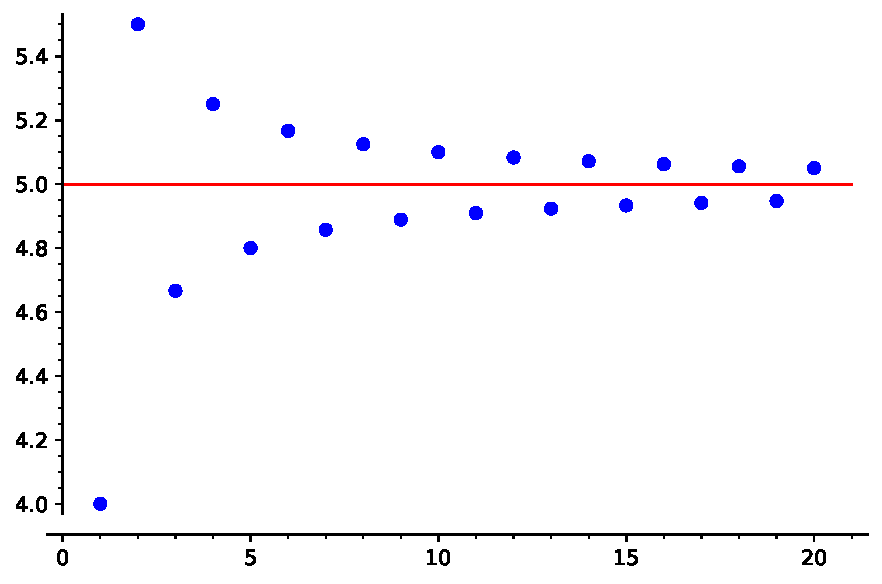
\includegraphics[width=0.7\textwidth]{code/grenzwert.pdf}
\end{center} 
\end{bem} 

\begin{bem} 
	Wir schauen uns den Begriff des Grenzwerts in Ruhe an. Die Bedingung $|a_n - a| < \epsilon$ können wir etwa als ``$a_n$ ist $\epsilon$-Approximation von $a$'' mit Worten beschreiben. Die Bedingung $n \ge n_0$ heißt ``$n$ muss groß genug sein'', mindestens so groß wie ein passend gewähltes $n_0$. Also beschreibt unsere Grenzwert-Definition die folgende Situation: egal welche Güte $\epsilon>0$ der Approximation des Wertes $a$ wir vorschreiben, wird diese Güte durch alle Glieder $a_n$ der Folge erreicht, bei denen der Index $n$ genügend groß ist. 
\end{bem} 

\begin{bem} Die Grenzwertbedingung 
\[ \lim_{n \to \infty} a_n = a
\] als eine quantifizierte Formel: 
	\[
			{\color{red} \forall \epsilon  \in \R_{>0} } \, {\color{blue} \exists n_0 \in \N } \, {\color{orange} \forall n \in \N : (n \ge n_0) \, \Rightarrow \,  } {\color{violet} |a_n - a| < \epsilon. }
	\]
	 {\color{red} Für jede Wahl  der positiven Genauigkeit} {\color{blue} gibt es einen Schwellenwert} {\color{orange} derart, dass für alle Indizes ab diesem Schwellenwert}	{\color{violet} die Glieder der Folge den Wert $a$ mit der gewünschten Genaugikeit approximieren}
\end{bem} 

\begin{bem} Die Bedingung, $a_n$ konvergiert nicht gegen $a$, heißt dementsprechend:  
	\[
	{\color{red} \exists \epsilon  \in \R_{>0} } \, {\color{blue} \forall n_0 \in \N } \, {\color{orange} \exists n \in \N : (n \ge n_0) \,  \wedge \,  } {\color{violet} |a_n - a| \ge  \epsilon. }
	\]
	{\color{red} Es gibt eine Wahl der Geauigkeit derart,} {\color{blue} dass nach jedem Index}  {\color{orange} ein weiterer mindestens so großer Index gefunden werden kann,} {\color{violet} für welchen das Folgenglied den Wert $a$ \textbf{nicht} mit der gewählten Genauigkeit approximiert}. 
	
	Mit anderen Worten: Für eine Wahl der Genauigkeit gibt es unendlich viele Folgenglieder, die den Wert $a$ mit der gewählten Genauigkeit \textbf{nicht} approximieren. 
\end{bem} 

\begin{bem}
	Ab wann $n$ genügend groß ist wird in der Definition durch eine natürliche Zahl $n_0$ vorgeschrieben. Streng genommen brauchen wir für den Wert $n_0$ nicht unbedingt Ganzzahligkeit. Daher findet man in der Literatur auch die folgende äquivalente Definition des Grenzwerts einer Folge: für jedes $\epsilon>0$ existiert ein $N \in \R$, sodass für alle $n \in \N$ mit $n \ge N$ die Ungleichung $|a_n - a| < \epsilon$ erfüllt ist. In dieser Definition ist $n_0$ durch eine reelle Zahl $N$ ersetzt.   
\end{bem} 

\begin{bem}
	Der Begriff des Grenzwerts einer Folge kann ganz analog über den Mengen eingeführt werden, in denen ein Abstandsbegriff festgelegt ist: die Bedingung $|a_n - a| < \epsilon$, dass der Abstand von $a_n$ und $a$. Für die komplexen Zahlen ist der Abstand von zwei  Zahlen ebenso der Betrag der Differenz dieser Zahlen. Also kann unsere Definition des Grenzwerts ohne Änderungen für folgen komplexer Zahlen benutzt werden. 
\end{bem} 

\begin{aufg}
Der Quotient $a_n = f_{n+1} / f_n$ der aufeinanderfolgenden Fibonacci-Zahlen ist ebenfalls eine Folge, über deren Eigenschaften für große $n$ man reflektieren könnte. Rechnen Sie die ersten Zehn Glieder $a_1,\ldots,a_{10}$ dieser Folge mit Computer/Taschenrechner in Gleitkomma-Arithmetik aus. Was stellen Sie experimentell fest? Sieht es wie eine konvergente Folge aus? Was könnte der Grenzwert sein? 
\end{aufg} 

\begin{bsp} {\ } 
	\begin{enuma} 
		\item In der Folge $a_n = 5 + \frac{(-1)^n}{n}$ schwanken die Glieder um die Zahl $5$ und liegen mal oberhalb mal unterhalb dieser Zahl. Der Grenzwert $\lim_{n \to \infty} a_n$ ist gleich $5$, weil die Abweichungen von $5$ für große $n$ beliebig klein werden. Wir können es auch formal aus der Definition des Grenzwerts herleiten. Sei $\epsilon>0$ gegeben. Wir können nun als $N = \frac{2}{ \epsilon}$ fixieren. Für alle $n \ge N$ gilt $|a_n - 5|  \le \frac{1}{2 \epsilon} < \epsilon$. 
		\item Die Folge $a_n = (-1)^n$ besteht aus Werten $-1$ und $1$, welche in dieser Folge abwechselnd auftreten. Diese Folge konvergiert gegen keinen Wert. Das ist intuitiv klar. Wenn die Folge für $n$ überhaupt was approximieren kann, dann nur $-1$ oder $1$, da der Wert beim wachsenden $n$ ständig zwischen $-1$ und $1$ wechselt, approximiert die Folge weder $-1$ noch $1$. 
	\end{enuma} 
\end{bsp} 

\begin{thm}[Eindeutigkeit des Grenzwertes] 
	Jede konvergente Folge hat genau einen Grenzwert. 
\end{thm} 

\begin{bem} Dieser Satz ist intuitiv klar: Eine konvergente Folge kann nur einen Wert approximieren. Wenn $a_n$ für große $n$ gleich zwei verschiedene Werte, etwa $0$ und $1$, approximieren würde, dann wäre $a_n$ gleichzeitig sehr nah an $0$ und sehr nah an $1$. Das geht natürlich nicht. 
\end{bem} 

\begin{defn}[Beschränktheit \& Monotonie] Eine Folge $(a_n)_{n \in \N}$ heißt: 
	\begin{enuma}
		\item \textbf{nach oben beschränkt}, wenn für eine Konstante $C$ die Ungleichung $a_n \le C$ für alle $n$ erfüllt ist;
		\item \textbf{nach unten beschränkt}, wenn für eine Konstante $c$ die Ungleichung $a_n \ge c$ für alle $n$ erfüllt ist. 
		\item \textbf{beschränkt}, wenn die Folge nach oben sowie nach unten beschränkt ist; 
		\item \textbf{monoton steigend}, wenn $a_n \le a_{n+1}$ für alle $n$ erfüllt ist;
		\item \textbf{strikt monoton steigend}, wenn $a_n < a_{n+1}$ für alle $n$ erfüllt ist;
		\item \textbf{monoton fallend}, wenn $a_n \ge a_{n+1}$ für alle $n$ erfüllt; 
		\item \textbf{strikt monoton fallend}, wenn $a_n > a_{n+1}$ für alle $n$ erfüllt ist; 
		\item \textbf{monoton}, wenn die Folge monoton steigend oder monoton fallend ist. 
	\end{enuma} 
\end{defn} 

\begin{thm}[Zusammenhang der Monotonie, Beschränktheit und Konvergenz] 
	\label{thm:monot:beschr:folgen} 
	Für Folgen reeller Zahlen gilt Folgendes: 
	\begin{enuma}
		\item \label{mon:beschr->konverg} Jede monotone, beschränkte Folge konvergiert. 
		\item Jede konvergente Folge ist beschränkt (aber im Allgemeinen, nicht umgekehrt). 
	\end{enuma} 
\end{thm} 

\begin{bem}
	Wenn wir in einer Folge endlich viele Glieder ändern, hat so eine Änderung keine Auswirkung auf Konvergenz und Grenzwert. Denn in der Definition des Grenzwert geht es um die genügend großen $n$. Man kann sich also auf so große $n$ einschränken, bei denen man nur die Glieder sieht die unverändert geblieben sind. Daraus folgt, dass wir 
	in der Behauptung \ref{mon:beschr->konverg} die Monotonie durch die Monotonie ab irgendeinem Glied ersetzen können: wenn eine Folge beschränkt und ab einem Glied monoton ist, ist sie konvergent. 
\end{bem} 

\begin{bsp} 
	Das Theorem gibt uns eine hinreichende und eine notwendige Bedingung für Konvergenz. Probieren wir es mal aus. 
	\begin{enuma}
		\item Die Folge $a_n = 2^{1/n}$ ist monoton und beschränkt. Je höher die Wurzel ist, die wir aus $2$ ziehen, desto kleiner ist das Ergebnis (daher die Monotonie). Beschränktheit ist ebenfalls klar, denn der Wert $2^{1/n}$ liegt offensichtlich zwischen $1$ und $2$. Auf diese Weise sehen wir dass die Folge $a_n$ konvergent ist, ohne dass wir den genauen Grenzwert dieser Folge angeben. Es kommen tatsächlich manchmal Situationen vor, in denen man weiß, dass der Grenzwert der vorliegenden Folge existiert, aber kein schöner einfacher Ausdruck für den Grenzwert vorhanden ist. So, weiß man zum Beispiel, dass der Grenzwert $\lim_{n \to \infty} (1+ 1/n)^n$ existiert, den Grenzwert kann man aber nicht ``elementar beschreiben''. Und so hat man einfach für diesen Wert den Buchstaben $e$ reserviert und den Wert die Euler-Zahl genannt. 
		\item Die Folge $a_n = n$ konvergiert nicht, denn diese Folge ist unbeschränkt. 
	\end{enuma} 
\end{bsp} 

\begin{thm}
	Die Folge $(1+ 1/n)^n$ ist konvergent. Der Grenzwert dieser Folge wird als $e$ bezeichnet und die Euler-Zahl genannt. 
\end{thm} 

\begin{bsp} 
	Kehren wir zurück zur Folge $2^{1/n}$. Wir bestimmen nun den Grenzwert dieser Folge. Wir zeigen, dass der Grenzwert gleich $1$ ist. Dafür sollen wir zeigen, dass für ein beliebiges festes $\epsilon>0$, die Ungleichung $|2^{1/n} - 1| < \epsilon$ für alle genügend großen $n$ erfüllt ist. Schreiben wir unsere Ungleichung ohne Betrag als eine untere und obere Schranke an $2^{1/n}$: 
	\[
		1 - \epsilon < 2^{1/n} < 1 + \epsilon. 
	\]
	Die untere Schranke ist für alle $n$ erfüllt, denn $2^{1/n}$ ist sogar durch $1$ nach unten beschränkt. Nun zur oberen Schranke: diese kann als $1/n < \log_2 (1 + \epsilon)$ und dann als $n > \frac{1}{\log_2 (1 +\epsilon) }$ umformuliert werden. Also ist die obere Schranke tatsächlich für alle genügend großen $n$ erfüllt. 
\end{bsp} 

\begin{defn}
	Eine nicht-konvergente Folge nennt man divergent. 
\end{defn} 

\begin{bem}
	Man muss aber an dieser Stelle etwas Ordnung in die Menge der divergenten Folgen bringen. Manche dieser Folgen gehen tatsächlich gegen keinen Wert, wie etwa $(-1)^n$, manche anderen gehen schon gegen etwas, aber dieses etwas ist kein reeller Wert. 
\end{bem} 

\begin{defn} 
	Man sagt, eine Folge $(a_n)_{n \in \N}$ \textbf{konvergiert gegen $\infty$}  (bzw. ist \textbf{bestimmt divergent gegen $+\infty$}), wenn für jede Schranke $C$ für genügend große $n$ überschritten wird: das heißt, für jede Konstante $C$ existiert ein $n_0$ derart, dass die Ungleichung $a_n > C$ für alle $n \ge n_0$ erfüllt ist. Komplett analog definiert man auch die bestimmte Divergenz gegen $-\infty$. 
\end{defn} 

\begin{bsp} {\ } 
	\begin{enuma}
		\item Die Folge $a_n = n$ konvergiert gegen $\infty$, das schreibt man als $\lim_{n \to \infty} n = \infty$. 
		\item  Die Folge $a_n = -n$ konvergiert gegen $-\infty$. Das schreibt man als $\lim_{n \to \infty} (-n) = -\infty$. 
		\item $\lim_{n \to \infty} \ln n = \infty$. 
		\item $\lim_{n \to \infty} (n + 2 (-1)^n) = \infty$. 
		\item Die Folge $a_n = (-1)^n n$ ist divergent, geht aber weder gegen $\infty$ noch gegen, denn $a_n$ schwankt für große $n$ zwischen großen positiven Werten und betragsmäßig großen negativen Werten. Der Betrag $|a_n| = n$ aber konvergiert gegen $\infty$. 
		\item Die Folge $a_n = ( 1 + (-1)^n) n$ schwankt für große $n$ zwischen $0$ und sehr großen Werten. Die Folge ist divergent und sie geht weder gegen $\infty$ noch gegen $-\infty$. 
	\end{enuma}
\end{bsp} 

\begin{bem}
	Auch eine nicht-monotone Folge kann gegen $\infty$ gehen. 
Hier die Folge $n+ 2 (-1)^n$.
	\begin{center}
			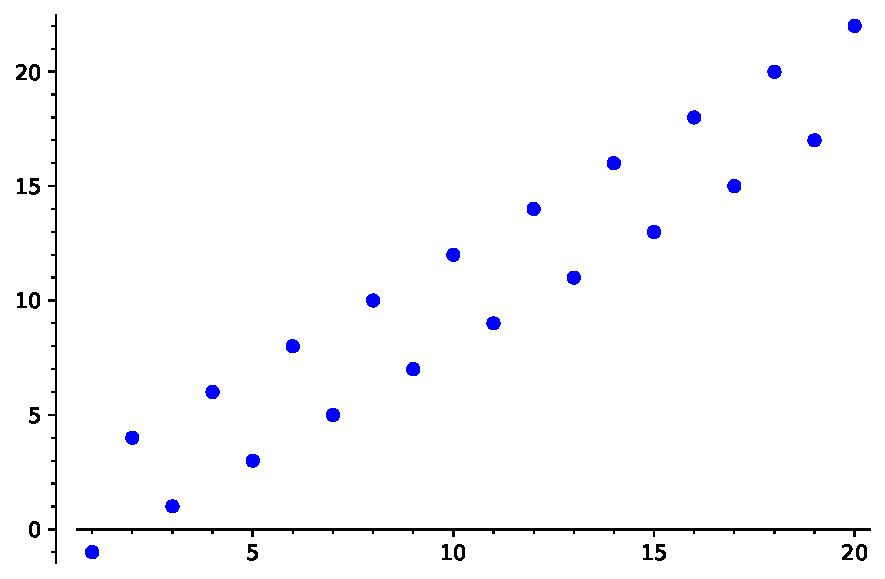
\includegraphics[width=0.7\textwidth]{code/gegen_unendlich.pdf}
	\end{center} 
\end{bem} 


%\begin{bsp} {\ } 
%	\begin{enuma}
%		\item Der Leitterm von $2 x^3 - 7 x^2 +8 x - 6$ ist $2 x^3$. 
%		\item Der Leitterm von $(2x-1)^{10}$ ist $(2x)^{10}$. (Wieso?)
%	\end{enuma} 
%\end{bsp} 

%\begin{bem} Eigentlich gibt es einen Unterschied zwischen Polynomen und Polynomialfunktionen. Polynome sind formale Ausdrücke und Polynomialfunktionen sind spezielle Abbildungen, aber im Kontext der Analysis ist dieser Unterschied nicht so wichtig, sodass wir Polynomialfunktionen auch einfach Polynome nennen werden. 
%\end{bem} 

%\begin{thm}
%	Seien $f, g$ Polynome mit Koeffizienten in $\R$ und sei $g$ nicht identisch gleich null. Dann 
%	gilt 
%	\[
%		\lim_{n \to \infty} \frac{f(n)}{g(n)}  = \lim_{n \to \infty} \frac{ (\text{Leitterm von $f$})(n)}{(\text{Leitterm von $g$})(n)}. 
%	\]
%\end{thm} 

\begin{bsp} 
	{\ } 
	\begin{enuma} 
		\item \[
			\lim_{n \to \infty} \frac{5 n^3 - 2n^2 + 7}{10 n^3 + 3 n^2+ 4 n+5}.
		\]
		\item 
		\[
			\lim_{n \to \infty} \frac{(2 n^2 + 1 )^3 }{(5 n^3 + n^2 - 1)^2}.
		\]
		\item 
			\[
				\lim_{n \to \infty} \frac{2 n + 1}{3  n^2 - 7 n + 6}.
		\]
		\item 
		\[
			\lim_{n \to \infty} \frac{n^2 + 100}{3 n-1000} .
		\]
	\end{enuma} 
\end{bsp} 

\begin{thm}[Rechenregeln für Folgen] 
	Für konvergente Folgen $(a_n)_{n \in \N}, (b_n)_{n \in \N}$ gilt: 
	\begin{enuma}
		\item $\lim_{n \to \infty} (a_n + b_n) = \lim_{n \to \infty} a_n + \lim_{n \to \infty} b_n $
		\item $\lim_{n \to \infty} (a_n \cdot b_n) = ( \lim_{n \to \infty} a_n) \cdot (\lim_{n \to \infty} b_n)$. 
		\item $\lim_{n \to \infty} b_n \ne 0$ $\Longrightarrow$ $\lim_{n \to \infty} \frac{a_n}{b_n} = \frac{\lim_{n \to \infty} a_n}{\lim_{n \to \infty} b_n}$. 
		\item Wenn $a_n \ge 0$ für alle $n \in \N$ und die Grenzwerte $\lim_{n \to \infty} a_n$ und $\lim_{n \to \infty} b_n$ sind nicht beide gleich $0$ $\Longrightarrow$ $\lim_{n \to \infty} a_n^{b_n} = (\lim_{n \to \infty} a_n )^{\lim_{n \to \infty} b_n}$. 
	\end{enuma} 
\end{thm} 

\begin{bem}
	\textcolor{red}{\textbf{WARNUNG!}}
	Wenn man mit Folgen mit Hilfe der obigen Regeln rechnet, soll man die Voraussetzungen beachten. Es kann passieren, dass $a_n + b_n$ konvergiert, auch wenn weder $a_n$ noch $b_n$ konvergieren. Zum Beispiel bei $a_n = - b_n = (-1)^n$. Die Summe $a_n + b_n = 0$ konvergiert gegen $0$, aber $a_n$ und $b_n$ konvergieren nicht. Wenn man also einer Folge etwa in die Summe von zwei Folgen ungünstig zerlegt hat, sodass die beiden Folgen divergent sind, heißt es noch lange nicht, dass die zugrundeliegende Folge divergent ist!
\end{bem} 

\begin{bem}[Unbestimmte Ausdrücke] 
	Interessant wird die Berechnung von Grenzwerten, in den Fällen, wo die vorigen Rechenregeln nicht eingesetzt werden können, weil die sogenannten unbestimmten Ausdrücke vorliegen. Dazu gehören z.B.: 
	\begin{itemize} 
			\item[] {\color{red} \glqq $\frac{0}{0}$ \grqq:}  $\lim_{n \to \infty} \frac{a_n}{b_n}$ mit $\lim_{n \to \infty} a_n = \lim_{n \to \infty} b_n= 0$. 
			\item[] {\color{red} \glqq$\frac{\infty}{\infty}$ \grqq:}   $\lim_{n \to \infty} \frac{a_n}{b_n}$ mit $\lim_{n \to \infty} a_n  = \infty $ und $\lim_{n \to \infty} b_n  = \infty$. 
			\item[] {\color{red} \glqq$1^\infty$ \grqq: } $\lim_{n \to \infty} (a^n )^{b_n}$ mit $\lim_{n \to \infty} a _n = 1$ und $\lim_{n \to \infty} b_n = \infty$. 
			\item[]  {\color{red} \glqq $\infty - \infty$ \grqq: } $\lim_{n \to \infty} (a_n -b_n)$ mit $\lim_{n \to \infty} a_n = \lim_{n \to \infty} b_n = \infty$. 
			\item[] {\color{red} \glqq$0^0$ \grqq: } $\lim_{n \to \infty} (a_n )^{b_n}$ mit $\lim_{n \to \infty} a _n = 0$ und $\lim_{n \to \infty} b_n = 0$. 
			\item[] {\color{red} \glqq$\infty^0$ \grqq: } $\lim_{n \to \infty} (a_n )^{b_n}$ mit $\lim_{n \to \infty} a _n = \infty$ und $\lim_{n \to \infty} b_n = 0$. 
	\end{itemize} 
	Grenzwerte für unbestimmte Ausdrücke lassen sich oft berechnen, indem man den die Unbestimmtheit des Ausdrucks durch äquivalente Umformungen auflöst und danach doch die Rechenregeln für Grenzwerte nutzen kann. 
	
	Eine weitere Technik, die helfen kann, ist die sogenannte Regel von l'Hospital, die auf dem Differenzieren basiert. 
\end{bem} 

\begin{aufg}
	Überlegen Sie sich, welche Werte die folgendne Grenzwerte haben. 
	\begin{enuma}
			\item $\lim_{n \to \infty} (\frac{1}{n})^{\frac{1}{n}}$
			\item $\lim_{n \to \infty} ( \frac{1}{2^n})^{1/n} $
			\item $\lim_{n \to \infty} ( \frac{1}{3^n})^{1/n} $
			\item $\lim_{n \to \infty} (\frac{1}{2^{n^2}})^{1/n}$. 
			\item $\lim_{n \to \infty} (\sqrt{n^2 + 3n +4} - \sqrt{n^2 + 2n + 3})$. 
	\end{enuma} 
\end{aufg} 



\begin{defn}[Teilfolge und ihr Grenzwert] 
	Eine \textbf{Teilfolge} über einer Menge $X$ besteht aus den Gliedern $a_{n_1} , a_{n_2}, a_{n_3},\ldots$ aus der Menge $X$, die durch ganze Zahlen $n_1 < n_2 < n_3 <  \cdots$ indexiert sind. 
	
	Der einzige Unterschied zu Folgen: Im Gegensatz zu Folgen sind die Glieder nicht unbedingt durchgängig nummeriert. Mit anderen Worten: Teilfolgen unterscheiden sich von den Folgen nur durch die Art der Nummerierung. 
	
	Die für Folgen eingeführten Begriffe wie \textbf{Grenzwert}, \textbf{Konvergenz} und \textbf{Divergenz} werden für Teilfolgen völlig analog definiert. 
\end{defn} 

\begin{bsp}
	$(a_p)_{p \ \text{ist Primzahl}}$ mit $a_p = \frac{1}{p^2}$ ist eine Teilfolge, die durch die Menge der Primzahlen indexiert ist. Man hat $a_2 = \frac{1}{4}, a_3 = \frac{1}{9}, a_5 = \frac{1}{25}$ usw. 
\end{bsp} 

\begin{defn} 
	Ist $(a_n)_{n \in \N}$ Folge und $1 \le n_1 < n_2 < n_2 \cdots $ unendlich viele Indizes, so nennt man $(a_{n_k})_{k \in \N}$ eine \textbf{Teilfolge der Folge} $(a_n)_{n \in \N}$. 
\end{defn} 


\begin{thm}
	Konvergiert eine Folge gegen einen Wert $a$, so konvergiert jede Teilfolge dieser Folge gegen den selben Wert $a$. 
\end{thm} 

\begin{bsp} {\ } Das vorige Theorem kann benutzt werden, um Divergenz nachzuweisen. 
	\begin{enuma} 
		\item Die Folge $a_n = (-1)^n$ ist divergent, denn 
		\begin{itemize} 
			\item[] die Teilfolge  $a_{n_k} = -1$ mit $n_k = 2k-1$ konvergiert gegen $-1$ und 
			\item[] die Teilfolge $a_{n_k} = 1$ mit $n_k = 2k$ konvergiert gegen den anderen Wert (die $1$). 
		\end{itemize} 
		\item Die Folge 
		\[
			a_n = \begin{cases} 
				1, & \text{$n$ Zweierpotenz},
				\\ 0, & \text{sonst}
			\end{cases} 
		\]
		ist divergent, denn 
		\begin{itemize} 
			\item[] die Teilfolge $a_{n_k} = 1$ mit $n_k = 2^k$ geht gegen $1$ und 
			\item[] die Teilfolge $a_{n_k} = 0$ mit $n_k = 2 k +1$ geht gegen $0$. 
		\end{itemize} 
	\end{enuma} 
\end{bsp} 

\section{Reihen} 

\begin{bem} 
	Salopp gesagt sind Reihen unendliche Summen. Etwas genauer sind es formale Summen der Glieder einer gegebener Folge. 
	
	Wir reden im Folgenden meistens über Reihen mit reellwertigen Gliedern. 
\end{bem} 

\begin{defn}[Reihe] Eine \textbf{Reihe} ist ein formaler Ausdruck der Form $\sum_{k=0}^\infty a_k$. 
	Die Elemente $a_k$ nennt man \textbf{Glieder} der Reihe. Die Glieder werden bei uns in der Regel reelle Werte sein. 
	
	Der Wert $s_n = \sum_{k=0}^n a_k$ ist \textbf{Partialsumme} zum Index $n$. 
	
	Eine Reihe nennt man \textbf{konvergent}, wenn die Folge $(s_n)_{n \in \N_0}$ der Partialsummen einen endlichen Grenzwert $s \in \R$ besitzt. In diesem Fall nennt man $s$ die Summe der Reihe und schreibt 
	\[
		\sum_{k=0}^\infty a_k = s. 
	\]
	Man benutzt in Bezug auf Reihen die gleiche Terminologie wie bei Folgen wie \textbf{divergent}, \textbf{bestimmt divergent gegen $\pm \infty$}, indem man sich dabei auf die Folge der Partialsummen bezieht. 
\end{defn} 

\begin{bem}
	Neben den Reihen mit den Gliedern, die ab $0$ indexiert sind, kann man natürlich auch Reihen betrachten, deren Gliedern ab einem anderen Wert indexiert sind. Neben der $0$ ist die $1$ ist ebenfalls sehr verbreitet. 
\end{bem} 

\begin{defn} 
	Eine \textbf{Nullfolge} ist eine Folge, die gegen $0$ konvergiert. 
\end{defn} 

\begin{thm}[Notwendige Bedingung für Konvergenz einer Reihe] 
	Die Folge der Glieder einer konvergenten Reihe ist eine Nullfolge. 
\end{thm} 

\begin{bem}
	Die Begründung zu diesem Theorem ist total einfach: hat $s_n = \sum_{k=0}^n a_k$ einen Grenzwert $s$ für $n \to \infty$, dann hat natürlich auch $s_{n-1}$ den Grenzwert $s$, für $n \to \infty$. Also ist $\lim_{n \to \infty} a_n = \lim_{n \to \infty} s_n - \lim_{n \to \infty} s_{n-1} = s-s = 0$. 
\end{bem} 

\begin{bsp} 
	Die Reihe $\sum_{k=1}^\infty (-1)^k$ ist divergent, da die Folge der Glieder nicht gegen $0$ konvergiert. In diesem Fall konvergiert die Folge der Glieder gar nicht. Wie sehen die Partialsummen dieser Reihe aus? 
\end{bsp} 


\begin{bsp} 
	Dass die Folge der Glieder gegen $0$ konvergiert, ist im Allgemeinen keine hinreichende Bedingung für die Konvergenz der Reihe. Betrachten wir die Reihe 
	\[
	1 + \underbrace{\frac{1}{2} + \frac{1}{2}}_{2 \ \text{mal}} + \underbrace{\frac{1}{3} + \frac{1}{3}+ \frac{1}{3}}_{3 \ \text{mal}}  +  \cdots +  \underbrace{\frac{1}{k} + \cdots + \frac{1}{k}}_{k \ \text{mal}} + \cdots 
	\]
	Das heißt, die Glieder sind $a_0=1$, $a_1 = a_2 = \frac{1}{2}$, $a_3=a_4=a_5 = \frac{1}{3}$ usw. Die Folge der Glieder geht gegen $0$. Die Summe der Reihe ist aber unendlich, denn die $k$ Glieder mit dem Wert $\frac{1}{k}$ ergeben insgesamt $k \cdot \frac{1}{k} = 1$. Da wir aber für jedes $k$, eine Gruppe aus $k$ Gliedern mit dem Wert $\frac{1}{k}$ haben, ist die Summe der Reihe unendlich. 
\end{bsp} 

\begin{bsp}[Harmonische Reihe] 
	Die Reihe $\sum_{k=1}^\infty \frac{1}{k}$ heißt harmonisch. Die Summe der Reihe ist unendlich! 
	
	\begin{center}
		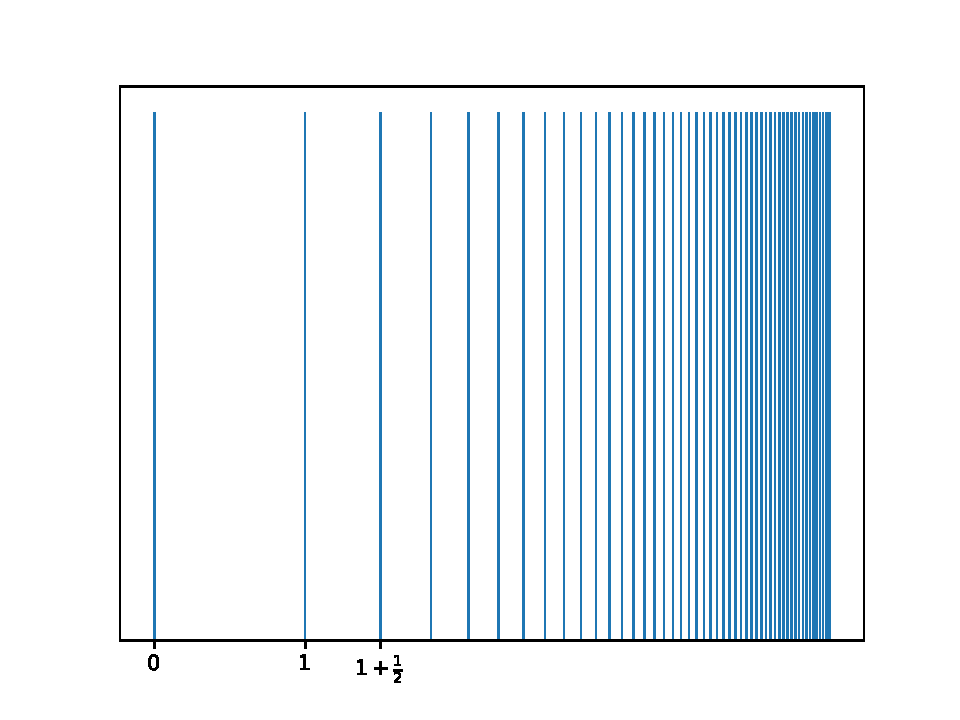
\includegraphics[width=0.8\textwidth]{pics/harmonic.pdf}
	\end{center}
	
	Wir zerlegen die Glieder in Gruppen, indem wir ab jeder Zweierpotenz eine neue Gruppe starten: 
 
	 Es gilt 
	
	\begin{align*}
		\sum_{k=1}^\infty \frac{1}{k} & = \sum_{i=0}^\infty \sum_{k=2^i}^{2^{i+1}-1} \frac{1}{k}
		\\ & \ge \sum_{i=0}^\infty \underbrace{\sum_{k=2^i}^{2^{i+1}-1} \frac{1}{2^{i+1}}}_{2^i \ \text{Terme}}
		\\ & = \sum_{i=0}^\infty 2^i \frac{1}{2^{i+1}}
		\\ & = \sum_{i=0}^\infty \frac{1}{2} 
		\\ & = \infty.  
	\end{align*}
\end{bsp} 

\begin{bem}
	Es stellt sich heraus, dass die Partialsumme $s_n = \sum_{k=1}^n \frac{1}{k}$ der harmonischen Reihe ziemlich gut durch den natürlichen Logarithmus $\ln n$ approximiert werden kann. 
	
	Hier $s_n$ im Vergleich zu $\ln x$ und $1 + \ln x$: 
	
	\begin{center}
			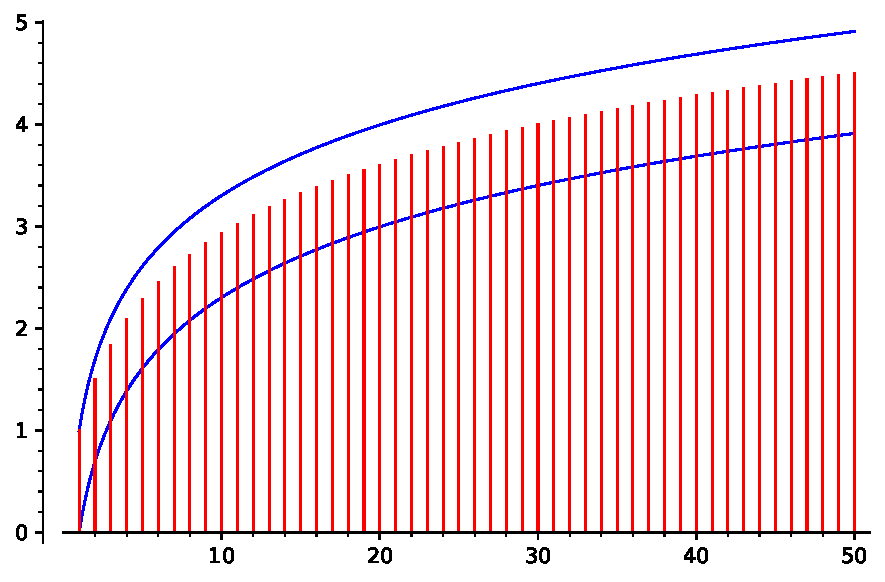
\includegraphics[width=10cm]{pics/partial_sums_harmonic_series.pdf} 
	\end{center} 
	
	Dass der QuickSort im Durchschnitt die Laufzeit der Ordnung $n \ln n$ hat, hängt auch mit der Partialsumme der harmonischen Reihe zusammen. Mehr Details dazu findet man im Buch von Cormen, Leiserson, Rivest und Stein ``Algorithmen: Eine Einführung''. 
\end{bem} 


\begin{bsp}[Geometrische Reihe] 
	Die geometrische Reihe $\sum_{k=0}^\infty q^k$ zu Basis $q \in \R \setminus \{1\}$ ist eines der bekanntesten Beispiele einer Reihe. Wir analysieren diese Reihe auf Konvergenz. Es ist nicht besonders schwer, eine abgeschlossene Formel für die Partialsummen 
	\[
		s_n = q^0 + \cdots + q^n
	\]
	zu erstellen. Der Wert $q s_n$ ist die Summe $q^1 + \cdots + q^{n+1}$. Wenn wir also von $q s_n$ die Summe $s_n$ abziehen, kompensieren sich die meisten Terme und man erhält $q s_n - s_n = q^{n+1} -1$. Somit ist 
	\begin{align}
		\label{eq:parti:geom:reihe}
		s_n = \frac{1 - q^{n+1}}{1-q}. 
	\end{align}
	Nun sieht man, dass die geometrische Reihe genau dann konvergiert, wenn $|q| < 1$ gilt. In der Tat: 
	\begin{enuma}
		\item Für $|q| < 1$, geht $q^n$ in der Darstellung \eqref{eq:parti:geom:reihe} von $s_n$ gegen $0$, woraus man $s_n \to \frac{1}{1-q}$ erhält. 
		\item Für $|q| \ge 1$, ist das Glied $q^k$ der Reihe keine Nullfolge, weil man $|q^k| \ge 1$ hat. 	Bei $|q| \ge 1$ kann noch zwischen der bestimmten Divergenz und unbestimmten Divergenz unterscheiden, denn: 
		\begin{itemize} 
			\item Bei $q>1$, geht $s_n$ gegen $\infty$. 
			\item Bei $q = -1$ geht die Partiasumme $s_n$ gegen ``gar nichts'':  sie zwischen zwei festen Werten. 
			\item Bei $q< -1$ schwankt die Partialsumme $s_n$ zwischen ``sehr positiven'' und ``sehr negativen'' Werten und geht somit ebenfalls gegen ``gar nichts''. 
		\end{itemize} 
	\end{enuma}
	
	Zusammenfassend: 	\(
	\sum_{k=0}^\infty q^k 
	\) ist
	\begin{enuma}
		\item bei $|q|<1$ der endliche Wert $\frac{1}{1-q}$ (die Reihe ist konvergent). 
		\item bei $q>1$ der unendliche Wert $+\infty$ (die Reihe ist bestimmt divergent gegen $+\infty$
		\item bei $q \le -1$ ``gar nichts'' (die Reihe ist unbestimmt divergent). 
	\end{enuma} 
\end{bsp} 

\begin{bsp}[Dezimaldarstellung von Zahlen] 
	Eigentlich ist die Darstellung von reellen Zahlen mit Hilfe von potenziell unendlich vielen Nachkommastellen ebenfalls eine Reihe. Wenn wir zum Beispiel die Zahl $0{,}\overline{1} = 0{,}1111\cdots$ betrachten, so meinen wir darunter die Summe der Reihe
	\[
		\sum_{k=1}^\infty \frac{1}{10^k}. 
	\]
	Schreiben Sie diese Zahl als Bruch.
	Bei allgemeinen Zahlen der Form $0{,}z_1 z_2 z_3 \cdots$ mit den Nachkommastellen $z_1,z_2,\cdots \in \{0,\ldots, 9\}$ ist die entsprechende Summe gleich 
	\[
		\sum_{k=1}^\infty \frac{z_k}{10^k}. 
	\]
\end{bsp} 

\begin{aufg} 
	Eine Programmfunktion wirft innerhalb einer While-Schleife iterativ eine faire Münze. Sobald eine Zahl geworfen wird, terminiert Ihre Funktion. Dabei ist der Rückgabewert $1$, wenn die Funktion nach einer ungeraden Anzahl der Iterationen terminiert hat, und $0$ sonst. Wie hoch ist die Wahrscheinlichkeit, dass die Funktion mit dem Rückgabewert $1$ terminiert? Was hat diese Wahrscheinlichkeit mit Reihen zu tun? 
	
	\underline{Hinweis:} Die elementare Wahrscheinlichkeitstheorie hatten Sie in der Schule. 
	
\begin{lstlisting} 
import random

KOPF=0
ZAHL=1

def unfaire_muenze():
	cntr=0
	while True: 
		cntr+=1
		if random.randint(KOPF,ZAHL)==ZAHL:
			return cntr % 2

# TEST
print([unfaire_muenze() for i in range(50)])
\end{lstlisting} 
	
\end{aufg} 

\begin{aufg} 
	Bestimmen Sie die Werte $z_1,z_2, z_3, z_4, \ldots \in \{0,1\}$ derart, dass die Gleichung 
	\[
		\sum_{k=1}^\infty \frac{z_k}{2^k}  = \frac{1}{3}
	\]
	erfüllt ist. 
	
	\underline{Hinweis:} Im Binärsystem kann man sehr bequem rechnen. Da Sie Informatiker/innen/ sind, muss das Binärsystem eines Ihrer Lieblingssysteme sein, oder? 
\end{aufg} 



\begin{bsp}
	Bei manchen elementaren Reihen, deren Glieder in rationaler Arithmetik erstellt werden, kommt erstaunlicherweise als Summe ein interessanter irrationaler Wert aus. Man hat zum Beispiel 
	\[
		\sum_{k=1}^\infty \frac{1}{k^2} = \frac{\pi^2}{6}. 
	\] 
	Wer hätte gedacht, das in einem so einfachen Ausdruck wie $\sum_{k=1}^\infty \frac{1}{k^2}$ die Kreiszahl versteckt ist! Wir könne diese Formel noch nicht herleiten, aber nach einigen Vorlesungen schon... 
\end{bsp} 

\begin{thm}[Linearkombination von Reihen] 
	Sind $\sum_{k=1}^\infty a_k$ und $\sum_{k=1}^\infty b_k$ konvergente Reihen, dann ist Ihre Linearkombination $\sum_{k=1}^\infty (\alpha a_k + \beta b_k)$ mit Koeffizienten $\alpha, \beta \in \R$ ebenfalls eine konvergente Reihe und es gilt: 
	\[
		\sum_{k=1}^\infty (\alpha a_k + \beta b_k) = \alpha \sum_{k=1}^ \infty a_k + \beta \sum_{k=1}^\infty b_k. 
	\]
\end{thm} 

\begin{defn}[Absolute Konvergenz]
	Eine Reihe $\sum_{n=1}^\infty a_n$ heißt \textbf{absolut konvergent}, wenn die Reihe $\sum_{n=1}^\infty |a_n|$ der Beträge der Glieder konvergent ist. 
\end{defn} 

\begin{thm}
	Jede absolut konvergente Reihe ist konvergent, aber im Allgemeinen nicht umgekehrt. 
\end{thm} 

\begin{bsp}
	$\sum_{n=1}^\infty \frac{(-1)^n}{n}$ ist konvergent, aber nicht absolut konvergent. 
\end{bsp} 


\begin{bem}
	\textcolor{red}{\textbf{WARNUNG!}} 
	Die konvergenten Reihen, die nicht absolut konvergent sind, sind ziemlich eigenartig!!! Ihr Grenzwert hängt zum Beispiel von der Reihenfolge der Glieder ab.
	
	Die absolut konvergenten Reihen sind dagegen ganz in Ordnung: sie sind im gewissen Sinne ähnlicher zu \underline{endlichen} Summen. 
\end{bem} 

\begin{bsp}
 Aus den  Werten der Menge  $M:=\{ \pm 1, \pm \frac{1}{2}, \pm \frac{1}{3}, \ldots \} $ kann man durch eine geeignete Anordnung der Werte eine Reihe erstellen, die eine beliebige von uns gewünschte Summe hat. Zum Beispiel: 
\begin{itemize}
	\item Starte mit $s_0:=0$ (vorige Patialsumme) und Zähler $n:=1$ (aktuelles Glied) sowie $i:=1$ (Index zum Verbrauch der positiven Werte) und $j:=1$ (Index zum Verbrauch der negativen Werte). 
	\item Iteriere unendlich wie folgt: 
	\begin{itemize} 
	\item[] Ist $s_{n-1} \le 20$,  setze $a_n := 1/i$ und $i:=i+1$, sonst setze $a_n:=-1/j$ und $j:=j+1$. 
	\item[] Generiere die nächste Partialsumme $s_n:=s_{n-1} + a_n$ und setze $n:=n+1$. 
	\end{itemize} 
	\item Ende der Iteration. 
\end{itemize} 
Dieses Verfahren produziert eine Reihe $\sum_{n=1}^\infty a_n$ mit der Summe $20$.  Hierbei werden alle Elemente von $M$ als Glieder von $a_n$ auftauchen, weil die harmonische Reihe $\sum_{k=1}^\infty \frac{1}{k}$ gleich $\infty$ ist, was dazu führt, dass man sowohl bei den negativen Elementen als auch bei den positiven Elementen aus $M$ nie aufhört, diese Elemente zu verbrauchen. 

Genauso könnte man aber an der Stelle von $20$ einen beliebigen Wert vorgeben, etwa $40$, und eine Reihe $\sum_{n=1}^\infty b_n$ produzieren, die bis auf die Änderung der Anordnung, dieselben Glieder aber eine andere Summe (die $40$) hat!
\end{bsp} 


\begin{bem}
	Wir wollen nun Produkte von Reihen einführen. Wir sind also an einer Reihe interessiert, die auf irgendeine Weise das Produkt 
	\[
		\left( \sum_{n=0}^\infty a_n \right) \left( \sum_{k=0}^\infty b_k \right) 
	\]
	von zwei Reihen darstellen soll. Wenn wir diesen Ausdruck formal ausmultiplizieren, so erhalten wir die formale Summe
	\[
		s:=\sum_{n,k \in \N_0} a_n b_k,
	\]
	in welcher Glieder nicht von einem sondern von zwei Indizes $n,k$ abhängig sind. Das heißt, die Glieder sind nicht durch aufsteigend geordnete ganze Zahlen indexiert, sondern durch Paare aus $\N_0^2$. Für die Paare ganzer Zahlen haben wir aber keine feste Anordnung. Bei der Diskussion der absoluten Konvergenz haben wir aber festgestellt, dass die Anordnung der Glieder im Allgemeinen Auswirkungen auf den Wert der Reihe hat. Das bedeutet, dass man das Produkt von allgemeinen konvergenten Reihen nicht (sinnvoll) einführen kann. Wenn man sich aber auf die absolut konvergenten Reihen einschränkt, hat man das beschriebene Problem nicht, sodass die formale Summe $s$ durch eine absolut konvergente Reihe beschrieben werden kann, zum Beispiel so: 
	\[
		s:= \underbrace{\color{red} a_0 b_0}_{c_0} + \underbrace{\color{blue} a_0 b_1 + a_1 b_0}_{c_1} + \underbrace{\color{orange} a_0 b_2 + a_1 b_1 + a_2 b_0}_{c_3} + \underbrace{\color{green} a_3 b_0 + a_2 b_1 + a_1 b_2 + a_0 b_3}_{c_3} + \cdots  . 
	\]
	Man zerlegt hier die Gesamtsumme der Werte $a_n b_k$ in Gruppen nach dem Wert von $n+k$. 
	
	\[
	\begin{array}{rrrrrrc}
		{\color{red} a_{0} b_{0} } & {\color{blue} a_{0} b_{1}} & {\color{orange} a_{0} b_{2} } & {\color{green} a_{0} b_{3}} & a_{0} b_{4} & a_{0} b_{5} & \cdots  \\
		{\color{blue} a_{1} b_{0}} &{\color{orange}  a_{1} b_{1}} & {\color{green} a_{1} b_{2} } & a_{1} b_{3} & a_{1} b_{4} & a_{1} b_{5} & \cdots \\
		{\color{orange} a_{2} b_{0} } & {\color{green} a_{2} b_{1}} & a_{2} b_{2} & a_{2} b_{3} & a_{2} b_{4} & a_{2} b_{5} & \cdots \\
		{\color{green} a_{3} b_{0}} & a_{3} b_{1} & a_{3} b_{2} & a_{3} b_{3} & a_{3} b_{4} & a_{3} b_{5} & \cdots \\
		a_{4} b_{0} & a_{4} b_{1} & a_{4} b_{2} & a_{4} b_{3} & a_{4} b_{4} & a_{4} b_{5} & \cdots \\
		a_{5} b_{0} & a_{5} b_{1} & a_{5} b_{2} & a_{5} b_{3} & a_{5} b_{4} & a_{5} b_{5} & \cdots \\
		\vdots & \vdots & \vdots & \vdots & \vdots & \vdots & \ddots 
	\end{array}
\]
\end{bem} 

\begin{defn}[Produkt absolut konvergenter Reihen] Das \textbf{Cauchy-Produkt} von zwei absolut konvergenten Reihen $\sum_{k=0}^\infty a_k$ und $\sum_{k=0}^\infty b_k$ is als die Reihe
\[
	\sum_{k=0}^\infty \underbrace{\left( \sum_{i=0}^k a_i b_{k-i} \right)}_{c_k}
\]
mit den Gliedern $c_0,c_1,c_2,\ldots$ definiert. 
\end{defn} 

\begin{thm} 
	Das Cauchy-Produkt von absolut konvergenten Reihen $\sum_{k=0}^\infty a_k$ und $\sum_{k=0}^\infty b_k$ ist eine absolut konvergente Reihe, für welche die Gleichung
	\[
		\sum_{k=0}^\infty \left( \sum_{i=0}^k a_i b_{k-i} \right) = \left( \sum_{k=0}^\infty a_k \right) \left( \sum_{k=0}^ \infty b_k \right) 
	\]
	erfüllt ist. 
\end{thm} 

\begin{bsp} 
	Jede konvergente geometrische Reihe ist absolut konvergent. 
\end{bsp} 

\begin{bsp}[Quadrat einer geometrischen Reihe. ] 
	Es gilt $\sum_{k=0}^\infty 2^{-k} =  2$. Da diese Reihe absolut konvergent ist (das ist klar - die Glieder sind nichtnegativ), können wir das Quadrat dieser Reihe als das Cauchy-Produkt der Reihe mit sich selbst  darstellen. Man hat 
	\begin{align*} 
		 2^{-0} 2^{-0} & = 1 \cdot 2^{-0}, 
		\\ 2^{-0} 2^{-1} + 2^{-1} 2^{-0} & = 2 \cdot 2^{-1}, 
		\\ 2^{-0} 2^{-2} + 2^{-1} 2^{-1} + 2^{-2} 2^{-0} & = 3 \cdot 2^{-2}
		\\ & \vdots 
	\end{align*}
	Es gilt also 
	\[
		4 = \left( \sum_{k=0}^\infty 2^{-k} \right)^2 = \sum_{k=0}^\infty (k+1) 2^{-k}.
	\]
	Das gibt uns die interessante Formel
	\[
		\sum_{k=1}^\infty k 2^{-k} = 2. 
	\]
\end{bsp} 

\begin{aufg} 
	Finden Sie eine Formel für $\sum_{k=0}^\infty k q^k$ im Fall $|q| < 1$. 
\end{aufg} 

\begin{aufg} 
	In einem Casino zahlen Sie für ein Spiel den Eintrittspreis von $g$ Euro und dürfen dann eine faire Münze solange werfen, bis sie eine Zahl geworfen haben. Haben Sie die Zahl das erste mal beim  $k$-ten Wurf erhalten, dann zahlt Ihnen das Casino $k$ Euro. Wenn Ihre Würfe zum Beispiel  Kopf, Kopf, Kopf, Kopf, Kopf, Zahl  waren, erhalten Sie $6$ Euro. 
	
	Was ist der faire Preis für dieses Spiel? Oder anders formuliert: bestimmen Sie für dieses Spiel den Wert $g^\ast$ derart, dass das Casino beim Eintrittspreis $g>g^\ast$ Geld (im Durchschnitt) gewinnt und beim Eintrittspreis $g<g^\ast$ Geld (im Durchschnitt) verliert. 
	
	\underline{Hinweise:} Die Wahrscheinlichkeitstheorie hatten Sie in der Schule. Es gibt mehrere Weisen, diese Aufgabe zu lösen, unter anderem eine sehr direkte Weise, die auf den oben diskutierten Formeln für Reihen basiert. 
\end{aufg} 

\begin{defn}
	Eine Reihe $\sum_{k=1}^\infty a_k$ mit $a_k a_{k+1} \le 0$ für alle $k \ge 0$ nennt man \textbf{alternierend}. 
\end{defn} 


\begin{bsp}
	Die Reihe $\sum_{k=1}^\infty \frac{(-1)^k}{k}$ ist ein Standardbeispiel einer alternierenden Reihe. 
\end{bsp} 

\begin{bem}
	Bis auf das Vorzeichen kann jede alternierende reellwertige Reihe als 
	\[
		\pm \sum_{k=1}^\infty (-1)^k a_k
	\] mit $a_k \ge 0$ für alle geschrieben werden. Der Faktor $(-1)^k$ im Glied der Reihe sorgt also für die Wahl des Vorzeichens des aktuellen Glieds $(-1)^k a_k$, während der Faktor $a_k$ den Betrag des Glieds bestimmt. 
\end{bem} 

\begin{thm}[Leibniz-Kriterium] 
	Ist $(a_k)_{k \in \N}$ eine monoton fallende Nullfolge nicht-negativer reeller Zahlen, dann ist die alternierende Reihe 
	\[
		\sum_{k=1}^\infty (-1)^k a_k
	\]
	konvergent. Darüber hinaus wird die Summe $s$ dieser Reihe durch die Partialsummen $s_n$ mit der folgenden Präzision approximiert: 
	\[
		|s - s_n | \le a_{n+1}. 
	\]
\end{thm} 

\begin{bem} 
	Die Glieder der alternierenden Reihe ``schwanken'' um den Nullwert. Das Leibniz-Kriterium besagt, dass im Fall von Schwankungen, die immer geringer werden und im Grenzwert verschwinden die zugrundeliegende Reihe konvergent ist. 
\end{bem} 


\begin{defn}
	Die Reihe $\sum_{k=0}^\infty b_k$ mit nichnegativen Gliedern $b_k$ nennt man eine \text{Majorante} der Reihe $\sum_{k=0}^\infty a_k$, wenn für ein $k_0$ die Ungleichung $|a_k| \le b_k$ für alle $k \ge k_0$ erfüllt ist. 
\end{defn} 

\begin{thm}[Majorantenkriterium] 
	Eine Reihe, die eine konvergente Majorante besitzt, ist absolut konvergent. 
\end{thm} 

\begin{defn}
	Die Reihe $\sum_{k=0}^\infty b_k$ mit nichnegativen Gliedern $b_k$ nennt man eine \text{Minorante} der Reihe $\sum_{k=0}^\infty a_k$, wenn für ein $k_0$ die Ungleichung $a_k \ge b_k$ für alle $k \ge k_0$ erfüllt ist. 
\end{defn} 

\begin{bsp}
	Wir analysieren die Reihe $\sum_{k=1}^\infty \frac{k}{3^k}$ auf Konvergenz: 
	\[
		\sum_{k=1}^\infty \frac{k}{3^k}\le \sum_{k=1}^\infty \frac{2^k}{3^k} = \sum_{k=1}^\infty \left( \frac{2}{3} \right)^k < \infty. 
	\]
	$\Rightarrow$ die Reihe $\sum_{k=1}^\infty \frac{k}{3^k}$ ist konvergent. 
\end{bsp} 

\begin{thm}[Minorantenkriterium]
	Eine Reihe, die eine divergente Minorante besitzt, ist divergent. 
\end{thm} 

\begin{bsp} 
	Wir analysieren die Reihe $\sum_{k=1}^\infty \frac{1}{\ln k}$ auf Konvergenz. 
	\[
		\sum_{k=1}^\infty \frac{1}{\ln k} \ge \sum_{k=1}^\infty \frac{1}{k} = \infty. 
	\]
	$\Rightarrow$ die Reihe $\sum_{k=1}^\infty \frac{1}{\ln k}$ ist divergent. 
\end{bsp} 

\begin{thm}[Quotientenkriterium für Konvergenz] 
	Gibt es für $\sum_{k=0}^\infty a_k$ Werte $k_0 \in \N$ und $0 \le q < 1$ derart, dass $\frac{|a_{k+1}|}{|a_k|} \le q$ für alle $k \ge k_0$ erfüllt ist, dann ist diese Reihe absolut konvergent. 
\end{thm} 

\begin{bsp} 
	$\sum_{k=1}^\infty \underbrace{\frac{k}{3^k}}_{= a_k}$ ist nach dem Quotientenkriterium konvergent, denn 
	\[
		\frac{|a_{k+1}|}{|a_k|} = \frac{(k+1) 3^k }{3^{k+1} k} = \left( 1 + \frac{1}{k} \right) \frac{1}{3} \le \underbrace{\frac{2}{3}}_{= q} < 1. 
	\]
\end{bsp} 

\begin{thm}[Quotientenkriterium für Divergenz] 
	Gibt es für $\sum_{k=0}^\infty a_k$  Werte $k_0 \in \N$ und $q> 1$ derart, dass $\frac{|a_{k+1}|}{|a_k|} \ge q$ für alle $k \ge k_0$ erfüllt ist, dann ist diese Reihe divergent. 
\end{thm} 

\begin{thm}[Quotientenkriterium für Konvergenz in der Grenzwertform]
	Gilt für die Reihe $\sum_{k=0}^n a_k$ die Ungleichung 
	\[
		\lim_{k \to \infty} \frac{|a_{k+1}|}{|a_k|} < 1,
	\]
	dann ist diese Reihe absolut konvergent. 
\end{thm} 

\begin{bsp}
	$\sum_{k=1}^\infty \underbrace{ \frac{k}{q^k} }_{=a_k}$ ist nach dem Quotientenkriterium konvergent für jedes $0 \le q < 1$, denn
	\[
		\lim_{k \to \infty} \frac{|a_{k+1}|}{|a_k|} = \lim_{k \to \infty} \frac{k q^{k+1}}{(k+1) q^k } = \lim_{k \to \infty} \left( 1 - \frac{1}{k+1} \right) q = q \in [0,1).
	\]
\end{bsp} 

\begin{thm}[Quotientenkriterium für die Divergenz in der Grenzwertform]
	Gilt für die Reihe $\sum_{k=0}^\infty a_k$ die Ungleichung 
	\[
	\lim_{k \to \infty} \frac{|a_{k+1}|}{|a_k|} > 1,
	\]
	dann ist diese Reihe divergent. 
\end{thm} 

\begin{bem}
	Bei $\lim_{k \to \infty} \frac{|a_{k+1}|}{|a_k|} =1$ kann man a priori nichts sagen: 
	\begin{itemize}
		\item[] Die Reihe $\sum_{k=1}^\infty \frac{1}{k}$ ist divergent und 
		\item[] $\sum_{k=1}^\infty \frac{1}{k^2}$ ist konvergent. 
	\end{itemize} 
\end{bem} 

\chapter{Grenzwerte und Stetigkeit von Funktionen} 

\section{Grenzwert einer Funktion} 

\begin{defn}
	Der topologische \textbf{Abschluss} $\overline{M}$ einer Teilmenge $M$ der reellen Zahlen ist die Menge der Grenzwerte konvergenter Folgen $(x_n)_{n \in \N}$ mit der Eigenschaft $x_n \in M$ für alle $n \in \N$. Eine Menge $M$ mit $M = \overline{M}$ nennt man \textbf{abgeschlossen}. 
\end{defn} 

\begin{bem} 
	$M$ ist stets eine Teilmenge von $\overline{M}$. 
\end{bem} 

\begin{bsp} {\ }
	\begin{enuma} 
		\item $[0,1]$ ist abgeschlossen. Mit anderen Worten: wenn eine Folge $(x_n)_{n \in \N}$ mit Werten aus $[0,1]$ einen Grenzwert besitzt, dann liegt dieser Grenzwert ebenfalls in $[0,1]$.  
		\item $[0,1)$ ist nicht abgeschlossen, denn $\overline{[0,1)} = [0,1]$. 
		\item Für $M = \setcond{ \frac{1}{t} }{t \in \N}$ gilt $\overline{M} = \{0\} \cup M$. 
	\end{enuma} 
\end{bsp} 

\begin{defn}
	Sei $p \in \R$ und $M$ Teilmenge von $\R$. Mann nennt $p$ \textbf{Häufungspunkt} von $M$, wenn $p$ im Abschluss von $M \setminus \{p\}$ liegt. 
\end{defn} 

\begin{bsp} {\ }
	\begin{enuma}
		\item Jeder Punkt von $[0,1]$ ist ein Häufungspunkt von $[0,1]$. 
		\item $0$ ist der einzige Häufungspunkt der Menge $M=\setcond{1/t}{t \in \N}$. Die Elemente von $M$ häufen sich nur in $0$, und nirgendwo sonst. 
		\item Alle Punkte aus $[0,1]$ sind Häufungspunkte von $M = [0,1] \cup \{2\}$. Es gibt keine anderen Häufungspunkte. Insbesondere ist der Punkt $2$ in $M$ kein Häufungspunkt von $M$. 
	\end{enuma} 
\end{bsp} 

\begin{defn}
	Sei $f : X \to \R$ Funktion und $a$ Häufungspunkt von $X$. Man sagt, dass $f$ für $x \to a$ gegen einen reellen Wert $y$ konvergiert, wenn für jedes $\epsilon>0$ ein $\delta >0$ existiert, für welches $|f(x) -y| < \epsilon$ für alle $x \in X$ mit $0 < |x-a| < \delta$ erfüllt ist. Schreibweise: $\lim_{x \to a} f(x) = y$. 
\end{defn} 

\begin{bsp}
	Die Funktion $f(x) = \frac{\sin x}{x}$ ist auf $\R \setminus \{0\}$ definiert. Die Null ist der Häufungspunkt des Definitionsbereiches. Es gilt: 
	\[
		\lim_{x \to 0} \frac{\sin x}{x} = 1. 
	\]
\end{bsp} 

\begin{bsp}
	$\lim_{x \to 0} x \sin ( 1/x) = 0$. 
\end{bsp} 


\begin{defn}
	Eine Funktion $f : X \to \R$ heißt
	\begin{enuma}
		\item \textbf{nach oben beschränkt}, wenn für eine Konstante $C \in \R$ die Ungleichung $f(x) \le C$ für alle $x \in X$ erfüllt ist. 
		\item \textbf{nach unten beschränkt}, wenn für eine Konstante $c \in \R$ die Ungleichung $f(x) \ge c$ für alle $x \in X$ erfüllt ist. 
		\item \textbf{beschränkt}, wenn $f$ nach oben und unten beschränkt ist. 
	\end{enuma} 
\end{defn} 

\begin{thm}
	Sei $f : X \to \R$ Funktion und $a$ Häufungspunkt von $f$. Konvergiert $f$ gegen $y$ für $x \to a$, so gilt $\lim_{n \to \infty} f(x_n) = y$ für jede Folge $(x_n)_{n \in \N}$ mit $x_n \in X \setminus \{a\}$ und $\lim_{n \to \infty} x_n  = a$. 
\end{thm} 

\begin{bsp} 
	Die Funktion $\sin(1/x)$ besitzt weder einen linksseitigen noch einen rechtseitigen Grenzwert im Punkt $0$, denn:  
	
	\begin{itemize}
		\item[] Für $x_n = \frac{1}{2 \pi n}$, gilt 
		\begin{align*}
			\lim_{n \to \infty} x_n & = 0,  & \lim_{n \to \infty} \sin(1/x_n) & = 0.
		\end{align*}
		\item[] Für $x_n = \frac{1}{2 \pi n + \frac{\pi}{2}}$, gilt \begin{align*}
				\lim_{n \to \infty} x_n & = 0, & \lim_{n \to \infty} \sin(1/x_n) & = 1. 
		\end{align*}
	\end{itemize} 
\end{bsp} 


\section{Stetige Funktionen und Unstetigkeiten} 

\begin{defn}
	Sei $f : X \to \R$ und 
	ei $a \in X$ Häufungspunkt von $X$. Mann nennt $f$ \textbf{stetig} in $a$, wenn $\lim_{x \to a} f(x) = f(a)$ gilt. Man nennt $f$ eine \text{stetige Funktion}, wenn die Funktion $f$ in jedem Punkt ihres Definitionsbereichs $X$ stetig ist. 
\end{defn} 

\begin{thm}
	Ist $f : X \to \R$ eine stetige Funktion so gilt für jede konvergente Folge $(x_n)_{n \in \N}$ mit $x_n \in X$ für alle $n$ und
	\[
		\lim_{n \to \infty} f(x_n) = f ( \lim_{n \to \infty} x_n). 
	\]
\end{thm} 

\begin{thm}
	Komposition, Produkt, Quotient und Summe stetiger Funktion sind stetige Funktionen. 
\end{thm} 

\begin{defn} 
	Eine \textbf{Polynomialfunktion} ist eine Funktion der Form 
	\[
	f(x) = c_d x^d + \cdots + c_0 x^0
	\] 
	mit Koeffizienten $c_d,\ldots,c_0$ und $d \in \N_0$. Sind alle Koeffizienten von $f$ gleich $0$, so setzen man den Grad $\deg(f)$ gleich $-\infty$. Ist $c_d \ne 0$, so definiert man den Grad von $f$ durch $\deg(f) = d$ und nennt den Term $c_d x^d$ den \textbf{Leitterm} von $f$. 
\end{defn} 


\begin{thm} Die folgenden Funktionen sind stetig: 
	\begin{enuma}
		\item Polynomialfunktionen und ihre Quotienten. 
		\item Funktionen $f(x) = x^a$ mit $a \in \R$ auf $(0,+\infty)$
		\item Exponentialfunktionen $f(x) = a^x$ mit $a > 0$,  
		\item Logarithmische Funktionen $f(x) = \log_a x$ mit $a > 0$ und $a \ne 1$, 
		\item Sinus, Kosinus, Tangens
		\item Arcus Sinus, Arcus Kosinus, Arcus Tangens.
	\end{enuma} 
\end{thm} 

\begin{defn}[Rechtsseitiger Grenzwert einer Funktion] 
	Sei $f : X \to \R$ Funktion auf $X \subseteq \R$ und $a \in \R$ Häufungspunkt von $X \cap [a,+\infty)$. Man  nennt $f$ konvergent für $x \to a+$, wenn ein Wert $y \in \R$ existiert mit der Eigenschaft, dass für jedes $\epsilon>0$ ein $\delta>0$ existiert, sodass für alle $x \in X$ mit $a < x < a + \delta$ die Ungleichung $|f(x) - y| < \epsilon$ erfüllt ist. 
	
	
	Den Wert nennt man den rechtsseitigen Grenzwert und bezeichnet als
	\[
	y = \lim_{x \to a+} f(x).
	\]
\end{defn}


\begin{defn}[Linksseitiger Grenzwert einer Funktion] 
	Sei $f : X \to \R$ Funktion auf $X \subseteq \R$ und $a \in \R$ ein Häufungspunkt von $X \cap (-\infty,a]$. 
	Der rechtsseitiger Grenzwert
	\[
	y = \lim_{x \to a-} f(x)
	\]
	ist ein Wert $y$ mit der Eigenschaft, dass für jedes $\epsilon>0$ ein $\delta>0$ existiert, sodass für alle $x \in X$ mit $a - \delta < x < a$ die Ungleichung $|f(x) - y| < \epsilon$ erfüllt ist. 
\end{defn}

\begin{bem}\ 
	Alternative Bezeichnungen für einseitige Konvergenz: 
		\begin{itemize} 
			\item[] $x \to a+$  schreibt man auch als $x \downarrow a$ und
			\item[] $x \to a-$ schreibt man auch als $x \uparrow a$.
		\end{itemize} 
\end{bem}  

\begin{bem} 
	Bestimmte Divergenz gegen $\infty$ und $-\infty$ für $x \to a + $ und $ x \to a^-$ kann analog zur bestimmten Divergenz für $x \to a$ eingeführt werden. 
\end{bem} 



\begin{thm}[Beschreibung der Konvergenz über die rechts- und linksseitige Konvergenz] 
	Sei $f : X \to \R$ und $a$  ein Häufungspunkt von $X \cap [a,+\infty)$ und $(-\infty,a] \cap X$. Dann sind die folgenden Bedingungen äquivalent: 
	\begin{enumi}
		\item $f(x)$ ist konvergent für $x \to a$. 
		\item $f(x)$ ist konvergent für $x \to a+$ und für $x \to a-$, und es gilt $\lim_{x \to a^+} f(x) = \lim_{x \to a^-} f(x)$. 
	\end{enumi}  
	Gegebenenfalls gilt $\lim_{x \to a} f(x) = \lim_{x \to a + } f(x) = \lim_{x \to a-} f(x)$. 
\end{thm} 

\begin{bsp}
	\begin{align*}
		\lim_{x \to 0+} \arctan \frac{1}{x} & = \frac{\pi}{2}, 
		\\ \lim_{x \to 0-} \arctan \frac{1}{x} & = - \frac{\pi}{2}. 
	\end{align*}
	$\Rightarrow$ $f(x)$ ist divergent für $x \to 0$. 
\end{bsp} 

\begin{defn} 
	Eine Menge $M \subseteq \R$, die beschränkt und abgeschlossen ist, nennt man \textbf{kompakt}. 
\end{defn} 

\begin{bsp} { \ } 
	\begin{enuma}
		\item $[a,b]$ ist kompakt für alle $a,b \in \R$ mit $a \le b$. 
	\end{enuma} 
\end{bsp} 

\begin{thm}[Satz von Weierstraß]
	Sei $f : [a,b] \to \R$ eine stetige Funktion auf einem kompakten Intervall. Dann erreicht die Funktion $f$ auf $[a,b]$ ihr Minimum und Maximum. Das heißt, es gibt $s,t \in X$ mit $f(s) \le f(x) \le f(t)$ für alle $x \in [a,b]$. 
\end{thm} 

\begin{thm}[Zwischenwertsatz] 
	Sei $f : [a,b] \to \R$ stetige Funktion auf einem  Intervall $[a,b]$ mit $a,b \in \R$ und $a<b$. Sei $f(a) \le y \le f(b)$ oder $f(b) \le y \le f(a)$. Dann existiert ein $\xi \in [a,b]$ mit $f(\xi) = y$. 
\end{thm}

\begin{bem} 
	Der Beweis vom Zwischenwertsatz basiert auf einem konstruktiven Ansatz. Man kann den Suchraum für $\xi$ iterativ halbieren und ein $\xi$ wie in der Behauptung beliebig gut approximieren. 
	
	\lstinputlisting{code/continuous_binary_search.sage}
	
	So ein algorithmischer Ansatz (der mit der binären Suche in sortierten Arrays verwandt ist) benötigt nur eine schwache Annahme über $f$ (Stetigkeit). Auch wenn $f$ nicht durch eine explizite Formel verfügbar ist sondern als ein sogenanntes Orakel zur Verfügung steht, mit dem man für ein gegebenes $x \in [a,b]$ den Wert von $f$ an der Stelle $x$ ermitteln kann, kann der Ansatz benutzt werden. 
	
	\begin{center}
	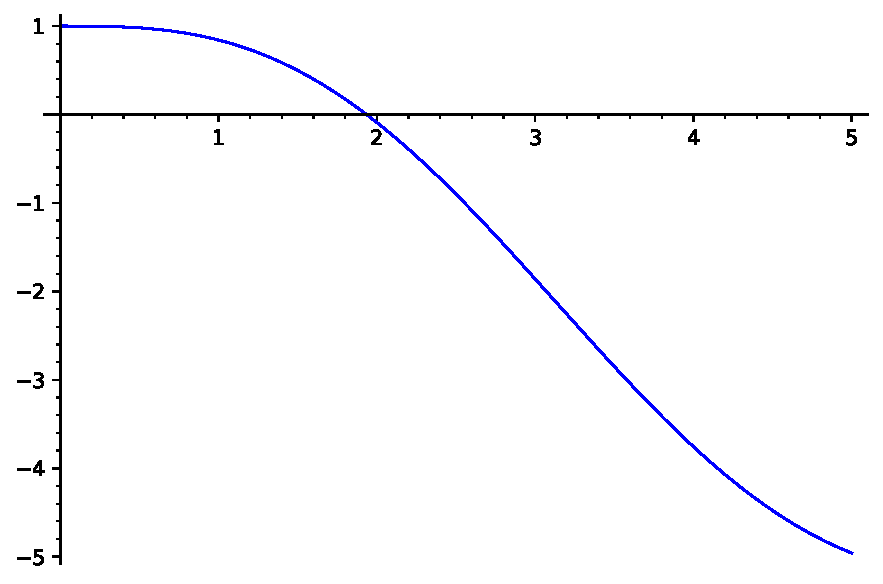
\includegraphics[width=10cm]{pics/continuous_binary_search_ex.pdf} 
	\\
	$\sin(x) + 1 - x$ besitzt eine Nullstelle in $[0,5]$, die mit Hilfe der ``stetigen'' binären Suche annähernd ermittelt werden kann. 
\end{center} 

\end{bem} 

\section{Asymptotisches Verhalten im Unendlichen} 

\begin{defn}
	Eine Teilmenge $M$ von $\R$ heißt
	\begin{enuma}
		\item \textbf{nach oben beschränkt}, wenn für eine Konstante $C \in \R$ die Ungleichung $x \le C$ für alle $x \in M$ erfüllt ist. 
		\item \textbf{nach unten beschränkt}, wenn für eine Konstante $c \in \R$ die Ungleichung $x \ge c$ für alle $x \in M$ erfüllt ist. 
		\item \textbf{beschränkt}, wenn $M$ nach oben und nach unten beschränkt ist. 
	\end{enuma}
\end{defn} 

\begin{defn}
	Sei $f : X \to \R$ Funktion auf einer Menge $X$, die nach oben nicht beschränkt ist. Mann nennt 
	$y$ den Grenzwert der Funktion $f(x)$ für $x \to \infty$, wenn für jedes $\epsilon>0$ ein $N \in \R$ existiert, für welches die Ungleichung $|f(x) - y| \le \epsilon$ für alle $x \in X$ mit $x \ge N$ erfüllt ist. Schreibwiese: $\lim_{x \to \infty} f(x) = y$. 
\end{defn} 

\begin{defn}
	Sei $f : X \to \R$ Funktion auf einer Menge $X$, die nach unten nicht beschränkt ist. Mann nennt 
	$y$ den Grenzwert der Funktion $f(x)$ für $x \to -\infty$, wenn für jedes $\epsilon>0$ ein $M \in \R$ existiert, für welches die Ungleichung $|f(x) - y| \le \epsilon$ für alle $x \in X$ mit $x \le M$ erfüllt ist. Schreibwiese: $\lim_{x \to -\infty} f(x) = y$. 
\end{defn} 

\begin{bsp} { \ } 
	\begin{enuma}
		\item $\lim_{x \to \infty} \left( 1 + \frac{1}{x} \right)^x = e$. Wir hatten bereits ein solches Beispiel mit einer Variablen $n$ aus $\N$. Nun haben wir eine Variable $x$, die innerhalb der \underline{reellen} Zahlen gegen $\infty$ geht. 
		\item $\lim_{x \to \infty} \arctan x  = \frac{\pi}{2}$ 
		\item $\lim_{x \to -\infty} \arctan x  = - \frac{\pi}{2}$ 
	\end{enuma} 
\end{bsp} 


\chapter{Differentialrechnung I}

Differentialrechnung für Funktionen einer Variablen

\section{Ableitung} 

\begin{defn}[Ableitung] 
	Sei $f : X \to \R$ und $a \in X$ Häufungspunkt von $X$. Man nennt $f$ \textbf{differenzierbar} in $a$, wenn ein endlicher Grenzwert
	\[
		f'(a) := \lim_{x \to a} \frac{f(x)-f(a)}{x-a}
	\]
	existiert. Man nennt $f'(a)$ die \textbf{Ableitung} von an der Stelle $a$. Somit ist die \textbf{Ableitung} $f'$ eine Funktion auf der Menge aller $a \in X$, in deren die Funktion $f$ differenzierbar ist. 
\end{defn} 

\begin{bem}
	Analog zum links- und rechtseitigen Grenzwert kann man auch die links- sowie rechtsseitige Ableitung an einer Stelle $a$ definieren: 
	\begin{align*}
			f'_l(x) & := \lim_{x \to a-} \frac{f(x)- f(a)}{x-a}, 
			\\ f'_r(x) & := \lim_{x \to a+} \frac{f(x) - f(a)}{x-a}. 
	\end{align*} 
	Für die Existenz der Ableitung von $f : \R \to \R$ in $a$ ist es notwendig und hinreichend, dass die links- sowie rechtsseitige Ableitung in $a$ existieren und und gleich sind. 
\end{bem} 

\begin{bem}
	Wenn man $h= x-a$ an der Stelle von $x$ benutzt, kann  man die Formel für die Ableitung als 
	\[
		f'(a) = \lim_{h \to 0} \frac{f(a+h) - f(a)}{h}
	\]
	umschreiben. 
	
	Man schreibt auch in manchen Quellen so: 
	\[
		f'(x) = \lim_{\Delta x \to 0} \frac{\Delta f}{\Delta x} 
	\]
	mit $\Delta f := f(x + \Delta x) - f(x)$. Hierbei ist 
	\begin{itemize} 
		\item[] $\Delta x$ eine (beliebig klein werdende) Änderung von $x$ und 
		\item[] $\Delta f$ die entsprechende Änderung von $f$ bzgl. einer festen Stelle $x$. 
	\end{itemize} 
\end{bem} 

\begin{bem}[Leibniz-Notation für die Ableitung und Differentiale] 
	Leibniz hat die Ableitung als einen formalen Quotienten geschrieben
	\[
		\frac{\dd f}{\dd x} = f'(x). 
	\]
 	Motivation zu dieser Bezeichnung: die Ableitung ist der Grenzwert eines \underline{Quotienten}. Diese Gleichung kann man auch formal auch als 
 	\[
 		\dd f = f'(x) \dd x.
 	\]
 	Hierbei nennt man $\dd f$ Differential von $f$ und $\dd x$ Differential von $x$. Das sind formale Symbole. Die intuitive Bedeutung dieser Gleichung ist: 
 	\[
 		\Delta f \approx f'(x) \Delta x.
 	\]
 	Das Vorige Bedeutet: $\Delta f = f'(x) \Delta x + o(\Delta x)$ mit $\frac{o(\Delta x)}{\Delta x} \to 0$ für $\Delta x \to 0$.  
\end{bem} 

\begin{bem}[Approximation, Tangente]
	Die (affin)lineare Funktion $f(a) + f'(a) (x-a)$ hat den gleichen Wert und die gleiche Ableitung in $a$ wie die Funktion $f$. Mit Hilfe des Wertes $f(a)$ von $f$ an der Stelle $f$ und der Ableitung von $f$ an der Stelle $a$ erhält man eine Approximation der Funktion $f$ in einer kleinen Umgebung der Stelle $a$. 
	
	Geometrisch gesehen beschreibt $y = f(a) + f'(a) (x-a)$ den Graphen der Tangente zum Graphen von $f$ an der Stelle $(a,f(a))$. 
\end{bem} 

\begin{bem} {\ } Einige physikalische Bedeutungen der Ableitung:
	\begin{enuma}
		\item Ist $f(t) \in \R$ die Position eines Objekts zum Zeitpunkt $t \in \R$, dann ist $f'(t)$ die Geschwindigkeit des Objekts im Zeitpunkt $t$. 
		\item Hat man auf der reellen Achse einen Stab $[0,L]$ der Länge $L>0$, bei dem die Masse des Abschnitts $[0,x]$ für $0< x < L$ gleich $m(x)$ ist, dann ist die Ableitung $\rho(x) = m'(x)$ die (lineare) Dichte im Punkt $x$. 
	\end{enuma} 
\end{bem} 

\begin{bsp} {\ } 
	Wir berechnen einige Ableitungen direkt aus der Definition. 
	\begin{enuma}
	\item Quadratische Funktion: 
	\[
		(x^2)' = \lim_{h \to 0} \frac{(x+h)^2 - x^2}{h} = \lim_{h \to 0} \frac{2 x h + h^2}{h} = \lim_{h \to 0} (2 x  + h) = 2 x. 
	\]
	\item Quadratische Wurzel: 
	\[
		(\sqrt{x})' = \lim_{h \to 0} \frac{\sqrt{x+h} - \sqrt{x}}{h} 
	\]
	Die Wurzel im Nenner stört, daher wir der Bruch mit $\sqrt{x+h} +  \sqrt{x}$ ergänzt, um von der Wurzel im Zähler loszuwerden. Mit der Verwendung der dritten binomischen Formel erhalten wir dann
	\[
		(\sqrt{x})' = \lim_{h \to 0} \frac{ (x+h) - x} { h (\sqrt{x + h} + \sqrt{x}) } = \lim_{h \to 0} \frac{1}{\sqrt{x+h} + \sqrt{x}} = \frac{1}{2 \sqrt{x}}.  
	\]
	Hierbei sollen wir voraussetzen, dass man $x> 0$ hat. 
	\item Die Funktion $1/x$: 
	\[
		(1/x)' = \lim_{h \to 0} \frac{1/(x+h) - 1/x}{h}. 
	\]
	Es bietet sich an, den Quotienten unter dem Grenzwert durch die Erweiterung mit $(x+h) x$ zu svereinfachen: 
	\[
		(1/x)'= \lim_{h \to 0} \frac{ x - (x+h)}{h (x+h) x} = \lim_{h \to 0} - \frac{1}{(x+h) x} =  - \frac{1}{x^2}. 
	\]
	Hierbei sollen wir $x \ne 0$ voraussetzen. 
	\end{enuma} 
\end{bsp} 

\begin{thm}
	Jede differenzierbare Funktion ist stetig, aber im Allgemeinen nicht umgekehrt. 
\end{thm} 

\begin{bem}
	Begründung zur Stetigkeit einer differenzierbaren Funktion ist wie folgt. Ist $f$ differenzierbar in $a$ so ist
	\[
		f'(a) = \lim_{x \to a} \frac{f(x) -f(a)}{x-a}
	\]
	ein endlicher Wert. Dann ist 
	\begin{align*}
		\lim_{x \to a} f(x) & = \lim_{x \to a} (f(x)-f(a)) + f(a)  & &|\text{ $f(a)$ abzeihen und wieder dazu addieren} 
		\\ & = \lim_{x \to a} \frac{f(x)-f(a)}{x-a} (x-a) + f(a)  & &| \text{ den Ableitungsquotienten zu erzeugen}
		\\ & = \lim_{x \to a} \frac{f(x)-f(a)}{x-a} \lim_{x \in a} (x-a) + f(a)  & &|  \text{ Produktregel für Grenzwerte}
		\\ & = f'(a) \cdot 0 + f(a) 
		\\ & = f(a) 
	\end{align*}
\end{bem} 


\begin{bsp} 
	$|x|$ ist stetig aber in $0$ nicht differenzierbar. 
\end{bsp} 

\begin{bem}
	Es gibt Beispiele von sehr unregelmässigen Funktionen, die auf $\R$ stetig aber an keiner Stelle differenzierbar sind. 
\end{bem} 

\begin{thm}[Rechenregeln für Differenzierbarkeit]
	Für differenzierbare Funktionen $f$ und $g$ gelten die folgenden Regeln: 
	\begin{enuma}
		\item Linearität: $(\alpha f + \beta g)'= \alpha f' + \beta g'$ mit $\alpha, \beta \in \R$
		\item Produktregel: $(f g)' = f' g + f g'$
		\item Quotientenregel: $\left( \frac{f}{g} \right)' = \frac{f' g  - f g'}{g^2}$
		\item Kettenregel: $(f \circ g)' = (f' \circ g) g'$.  
	\end{enuma}
\end{thm} 


\begin{bem}
	Intuition hinter der Produktregel ist wie folgt. Die Änderung des Produkts ist: 
	\begin{align*}
		\Delta (f g) & = (f+\Delta f) ( g + \Delta g) - f g & & |\text{ Ausmultiplizieren} 
		 \\ & = (\Delta f) g  + f (\Delta g ) + (\Delta f) (\Delta g).
	\end{align*}
	Wenn $\Delta f$ und $\Delta g$ klein sind, dann ist $(\Delta f) (\Delta g)$ noch kleiner und somit zu klein. Wenn $f$ und $g$ Funktionen in $x$ sind und man durch $\Delta x$ teilt und dann $\Delta x$ gegen $0$ schickt, erhält man 
	\[
		(f g)' = f' g + f g'.
	\]
	Die Produktregel hängt also direkt mit der Approximationsformel
	\[
		\Delta (f g) \approx(\Delta f) g + f (\Delta g)
	\]
	zur Änderung eines Produkts zusammen. Mit Worten lautet die Formel: durch eine kleine Änderung der beiden Faktoren in einem Produkt  ergibt sich die Änderung des Produkts im Wesentlichen aus der Änderung des ersten Faktors mal der zweite Faktor und die Änderung des zweiten Faktors mal der erste Faktor. 
	
	Eine solche Formel nutzt man gerne in den Naturwissenschaften bei Experimenten, wenn man bei der Messung von zwei Größen jeweils den aditiven Fehler der Messung abgeschätzt hat und darauf basierend den Fehler des Produkts für die beiden Größen abschätzen möchte. 
\end{bem} 

\begin{bsp}[zu Produktregel] 
	\begin{align*}
		(x^2 \sin x)' & = (x^2)' \sin x + x^2 (\sin x)'  & & |\text{ Produktregel}
		\\ & = 2 x \sin(x)+ x^2 \cos(x). & & |\text{ Formeln für $(x^2)'$ and $(\sin x)'$} 
	\end{align*}
\end{bsp} 

\begin{bem} 
	Intuition hinter der Quotientenregel: 
	\begin{align*}
	\Delta \left( \frac{f}{g} \right) & = \frac{ f + \Delta f}{g + \Delta g} - \frac{f}{g}  & & |\text{ Aus der Def. von $\Delta$ einer Funktion} 
	\\ & = \frac{(f+ \Delta f) g - f (g + \Delta g) }{ g (g + \Delta g)} 
	& & |\text{ Als ein Quotient umgeschrieben}
	\\ & =  \frac{(\Delta f) g - f \Delta g }{g (g + \Delta g)} & & 
	|\text{ Klammern aufgelöst, $fg$ verschwindet.}
	\end{align*}
	Wenn man durch $\Delta x$ teilt und dann $\Delta x$ gegen $0$ schickt, erhält man: 
	\[
	\left( \frac{f}{g} \right)' = \frac{f' g - f g'}{g^2}. 
	\]
\end{bem} 


\begin{bsp}[zu Quotientenregel]
	\begin{align*}
		\left( \frac{\sin x}{x^2} \right)' & = \frac{ (\sin x)'   x^2 - \sin x (x^2)'}{(x^2)^2} 
		\\ & = \frac{x^2 \cos x - 2 x \sin x}{x^4}
		\\ & = \frac{ x \cos x - 2 x \sin x}{x^3}. 
	\end{align*}
\end{bsp} 

\begin{bsp}[Intuition hinter der Kettenregel an einem Beispiel]
	Wir berechnen die Ableitung von $z(x) = \sin (x^2)$, wie es Leibniz gemacht hätte. Man hat $z = \sin y$ und $y = x^2$. 
	\begin{align*}
		\frac{\dd z}{\dd x} & = \frac{\dd z}{\dd y} \cdot \frac{\dd y}{\dd x}. &  & \text{(Ableitung ist ``Quotient'', wir ergänzen formal)}
		\\ & = (\frac{\dd}{\dd y} \sin y) \cdot (\frac{\dd}{\dd x} x^2)
		\\ & = (\cos y) \cdot (2 x)
		\\ & = (\cos x^2) \cdot (2 x)
		\\ & = 2 x \cos x^2.
	\end{align*}
	Wie man es sonst schreibt is:
	\[
		(\sin x^2)' = (\cos x^2) \cdot (x^2)' = (\cos x^2) \cdot (2 x) = 2 x \cos x^2. 
	\]
\end{bsp} 

\begin{bsp}[Kettenregel für längere Ketten]
	Hier ein Beispiel, in dem man drei Funktionen ineinander geschachtelt hat (Sinus, e hoch, Quadrat): 
	\begin{align*}
		(\sin e^{x^2})' & = (\cos e^{x^2} ) \cdot (e^{x^2})' 
		\\ & = (\cos e^{x^2} ) \cdot e^{x^2} \cdot (x^2)' 
		\\ & = (\cos e^{x^2} ) \cdot e^{x^2} \cdot (2 x ). 
	\end{align*}
\end{bsp}

\begin{aufg}
	Leiten Sie eine Produktregel für die Ableitung des Produkts von $n \in \N$ Funktionen $f_1,\ldots, f_n$ her und nutzen Sie diese Regel um die Ableitung von $e^x (\ln x) (\sin x) x^2$ zu bestimmen. 
\end{aufg} 

\begin{aufg}
	Leiten Sie eine Verallgemeinerung der Quotientenregel für die Funktion $f_1 \cdot f_n / g$ her, die als Quotient des Produkts von $n \in \N$ Funktionen $f_1,\ldots,f_n$ und einer Funktion $g$ gegeben ist. 
\end{aufg} 

\begin{aufg}
	Überprüfen Sie, ob die Funktionen $|x|^3, |x|^2, |x|, \cos|x|, \tan |x|, x^2 \sin |x|$ an der Stelle $0$ differenzierbar sind. 
\end{aufg} 

\begin{thm}[Ableitung der Umkehrfunktion] 
	Seien $I, J$ Intervalle. Für eine bijektive differenzierbare Funktion $ f : I \to J$ ist die Umkehrfunktion überall, wo $f' \circ f^{-1}$ ungleich $0$ ist, differenzierbar, und es gilt: 
	\[
		(f^{-1})' = \frac{1}{f' \circ f^{-1}}. 
	\]
\end{thm} 

\begin{bsp}[Leibniz'sche Intuition an einem Beispiel]
	Wir kennen, dass $(e^x)' = e^x$ gilt. 
	Die Gleichung 
	\[
		y = e^x
	\]
	kann man auch als $x = \ln y$ um schreiben. Man hat 
	\[
		\frac{\dd y}{\dd x} = \frac{\dd}{\dd x} e^x = e^x. 
	\]
	Das schreiben wir wie Leibniz formal um: 
	\[
		\frac{\dd x}{\dd y} = e^{-x} = (e^x)^{-1} = y^{-1}. 
	\]
	Da wir $x = \ln y$ haben, erhalten wir 
	\[
		\frac{\dd }{\dd y}  \ln y  = \frac{1}{y}. 
	\]
	Das heißt, aus der Formel für die Ableitung der Exponentialfunktion erhalten wir die Formel für die Ableitung für den Logarithmus. 
	
	Nach diesem Prinzip kann man für Umkehrfunktion bekannter Funktionen Formeln für die Ableitungen bestimmen. 
\end{bsp} 


%\begin{bem}[Begründung] $(f \circ f^{-1})(x) = x$ nach der Definition der Umkehrfunktion. Die Ableitung von $x$ ist $1$. Das Ableiten mit der Verwendung der Kettenregel ergibt also $1 = (f' \circ f^{-1} ) \cdot (f^{-1})'$. 
%\end{bem} 

%\begin{bem} 
%	Wir wenden dieses Prinzip an, um die Ableitung von $\ln x$ aus $(e^x)' =e^x$ auszurechnen. Es gilt $x = e^{\ln x}$. Es gilt: 
%	\[
%		1 = x' = (e^{\ln x})' = e^{\ln x} \cdot (\ln x)'  = x \cdot (\ln x)'. 
%	\]
%	Das zeigt $(\ln x)' = 1/x$. 
%\end{bem} 


\begin{thm} Es gelten die folgenden Formeln für die Ableitungen: 
	\begin{itemize}
		\item[] $(x^a)' = a x^{a-1}$ für $a \in \R$. 
		\item[] $(e^x)'  = e^x$
		\item[] $(\ln x)' = \frac{1}{x}$. 
		\item[] $(\sin x)' = \cos x$
		\item[] $(\cos x)' = - \sin x$
		\item[] $(\tan x)' = - \frac{1}{(\cos x)^2}$. 
		\item[] $(\arcsin x)' = \frac{1}{\sqrt{1-x^2}}$
		\item[] $(\arccos x)' = - \frac{1}{\sqrt{1-x^2}}$
		\item[] $(\arctan x)' = \frac{1}{1+x^2}$. 
	\end{itemize} 
\end{thm} 

	\begin{aufg} 
		Bestimmen Sie: 
		\begin{enuma}
			\item $(a^x)'$ aus $(e^x)' = e^x$ und der Kettenregel. 
			\item $(x^a)'$ aus $(e^x)' = e^x$ und der Kettenregel. 
			\item $(\sin x)'$ aus $\lim_{x \to 0} \frac{\sin x}{x} = 1$ und den trigonometrischen Formeln. 
			\item $(\cos x)'$ aus $(\sin x)' = \cos x$ und den trigonometrischen Formeln. 
			\item $(\tan x)'$ aus der Quotientenregel und den trigonometrischen Formeln.
			\item die Formeln für die Ableitung der inversen trigonometrischen Funktionen aus den Formeln für die Ableitung der trigonometrischen Funktionen. 
		\end{enuma} 
	\end{aufg} 

\begin{aufg} 
	In der Formel $(\ln x)' =\frac{1}{x}$ ist $x$ auf den Fall $x>0$. Im Gegensatz dazu lässt $\ln |x|$ für alle $x \in \R \setminus \{0\}$ auswerten? Bestimmen Sie die Ableitung von $\ln |x|$. 
	 \textbf{Hinweis:} obwohl $|x|$ durch eine Fallunterscheidung definiert ist, hat man eine Formel für die Ableitung von $\ln |x|$, die keine Fallunterscheidung benötigt. 
\end{aufg} 

\begin{thm}[Regel von l'Hospital]
	Seien $f, g : X \to \R$ differenzierbare Funktionen. Sei $a \in \R$ Häufungspunkt von $X$ oder $a=\infty$ und $X$ nach oben unbeschränkt oder $a = -\infty$ und $X$ nach unten unbeschränkt. Sei $\lim_{x \to a} f(x) = \lim_{x \to a} g(x) = 0$ oder $\lim_{x \to a} |f(x)| = \lim_{x \to a} |g(x)| = \infty$. 
	
	Wenn der Quotient $\frac{f'(x)}{g'(x)}$ für $x \to a$ konvergent ist, dann ist der Quotient $\frac{f(x)}{g(x)}$ für $x \to a$ ebenfalls konvergent ist, und es gilt: 
	\[
		\lim_{x \to a} \frac{f(x)}{g(x)} = \lim_{x \to a} \frac{f'(x)}{g'(x)}. 
	\]  
\end{thm} 

%\begin{defn} 
%	Einen Punkt $x$ in einer Teilmenge $M$ reeller Zahlen nennt man \textbf{isoliert}, wenn ein $\epsilon>0$ existiert, für welches $|x - y| \ge \epsilon$ für alle $y \in M$ mit $y \ne x$ erfüllt ist.  
%\end{defn} 


\begin{bsp} {\  } 
	\begin{enuma} 
		\item $\lim_{x \to 0} \frac{\sin x}{e^x - 1} \stackrel{\text{l'H}}{=} \lim_{x \to 0} \frac{(\sin x)'}{ (e^x - 1)'} = \lim_{x \to 0} \frac{\cos x}{ e^x} = \frac{1}{1} = 1$. 
		\item $\lim_{x \to 0} \frac{x^2}{1 - \cos x} \stackrel{\text{l'H}}{=} \lim_{x \to 0} \frac{ (x^2)'}{ (1- \cos x)'} = \lim_{x \to 0} \frac{ 2 x }{ \sin x} \stackrel{\text{l'H}}{=} \lim_{x \to 0} \frac{(2 x)'}{(\sin x)'}  = \lim_{x \to 0} \frac{ 2}{ \cos x} = 2.$ 
	\end{enuma} 
\end{bsp} 

\begin{bsp}[Intuition hinter der Regel von L'Hospital an einem Beispiel]
	\[
		\lim_{x \to 0} \frac{\sin x}{e^x - 1} =\lim_{x \to 0} \frac{ \frac{ \sin x - \sin 0}{x - 0} }{ \frac{e^x - e^0}{x-0} } = \frac{\lim_{x \to 0} \frac{ \sin x - \sin 0}{x - 0}}{\lim_{x \to 0} \frac{e^x - e^0}{x-0}}  = \frac{(\sin x)'|_{x=0}}{ (e^x)'|_{x =0}} = \frac{\cos 0}{ e^0} = 1. 
	\]
\end{bsp} 

\begin{defn}[Höhere Ableitungen] 
	Für eine Funktion $f : X \to \R$ auf $X \subseteq \R$, wird die $n$-te Ableitung von $f$ rekursiv definiert: 
	\[
	f^{(n)} := \begin{cases} 
	f, & \text{für} \ n =0,
	\\ (f^{(n-1)})', & \text{für} \ n \in \N. 
	\end{cases} 
	\]
	Das heißt: $f^{(0)} = f$, $f^{(1)} = f'$, $f^{(2)} = f''$ usw. 
\end{defn} 

\begin{bem}
	In Physik, Wirtschaftswissenschaft und anderen Anwendungsbereichen betrachtet man oft zeitliche Veränderungen verschiedener Größen. 
	
	Dabei benutzt man oft die Ableitungen der Größen nach der Zeit, um solche Veränderungen formal und/oder quantitativ zu beschreiben. Wen wir $f(t)$ betrachten und  $t$ Zeit ist, so ist: 
	\begin{itemize} 
		\item $f(t)$ - der Wert $f$ zum Zeitpunkt $t$. 
		\item $f'(t)$ - die Geschwindigkeit von $f(t)$, $f'(t)>0$ - Wachstum, $f'(t)<0$ - Abnahme. 
		\item $f'(t)$ - Beschleunigung von $f(t)$. 
	\end{itemize} 
\end{bem} 

\begin{bem}
	In den Nachrichten findet man immer wieder Berichte, die indirekt einen Bezug zu höheren Ableitungen haben. Z.B. ``Wachstum beschleunigt sich'' heißt $f'(t)>0$ (Wachstum) und $f'''(t)>0$ (Beschleunigung des Wachstums). 
\end{bem} 

\begin{bsp} 
	Weil für $f(x)=e^x$ man $f'(x) = e^x = f(x)$ hat, gilt $f^{(n)}(x) = e^x$ für alle $n \ge 0$. 
\end{bsp} 

\begin{bsp} 
	Für $f(x) = x^a$ mit $a \in \R$ gilt 
	\[
		f^{(n)}(x) = a \cdot (a-1) \cdot \ldots \cdot (a-n+1) x^{a-n}. 
	\]
	Insbesondere: für $a \in \N_0$ hat man $f^{(a)}(x) = a!$ und $f^{(n)}(x)=0$ für $n > a$. 
\end{bsp} 

\begin{bsp} 
	Für $f(x) = \sin x$ gilt $f^{(4)}(x) = f(x)$. Es folgt: $f^{(n)}(x)$ $4$-periodisch in $n$. Das heißt, $f^{(n+4)}(x) = f^{(n)}(x)$. 
\end{bsp} 



\begin{bem} 
	Ist $f(t) \in \R$ die Position eines Objekts auf der reellen Achse im Zeitpunkt $t \in \R$, dann ist $f'(t)$ die Geschwindigkeit im Zeitpunkt $t$ und $f''(t)$ die Beschleunigung im Zeitpunkt $t$. 
	
	Zweite Ableitungen spielen eine wichtige Rolle in der Physik (das zweite Gesetz von Newton: Kraft $=$ Masse $\times$ Beschleunigung). 
\end{bem} 

\section{Monotonie und Extremwerte} 

\begin{defn}
	Eine Funktion $f : X \to \R$ auf $X \subseteq \R$ heißt: 
	\begin{enuma}
		\item \emph{monoton steigend}, wenn für alle $x, y \in X$ mit $x \le y$ die Ungleichung $f(x) \le f(y)$ erfüllt ist; 
		\item \emph{strikt monoton steigend}, wenn für alle $x, \in X$ mit $x<y$ die Ungleichung $f(x)<f(y)$ erfüllt ist;
		\item \emph{monoton fallend}, wenn für alle $x,y \in X$ mit $x \le y$ die Ungleichung $f(x) \ge f(y)$ erfüllt ist;
		\item \emph{strikt monoton fallend}, wenn für alle $x, y \in X$ mit $x<y$ die Ungleichung $f(x)> f(y)$ erfüllt ist. 
	\end{enuma} 
\end{defn} 

\begin{thm} Sei $f: I \to \R$ differentierbare Funktion auf einem offenen Intervall $I$. Dann gilt: 
	\begin{enuma} 
		\item $f$ monoton steigend $\Leftrightarrow$ $f'$ nicht-negativ.
		\item $f'$ monoton fallend $\Leftrightarrow$ $f'$ nicht-positiv. 
	\end{enuma} 
\end{thm} 

\begin{bem}[Begründung der Richtungen ``$\Rightarrow$'']
	Sei $a \in I$. 
	
	Ist $f$ monoton steigend, so gilt $\frac{f(x) - f(a)}{x-a} \ge 0$ für alle $x \in I$ mit $x \ne a$. Also ist
	\[
		f'(a) = \lim_{x \to a} \frac{f(x) - f(a)}{x-a},
	\]
	als der Grenzwert einer nicht-negativen Ausdrucks, nicht-negativ. 
	
	Analog ist bei einer monoton fallenden Funktion $f$ die Ableitung $f'(a)$, als der Grenzwert eines nicht-positiven Ausdrucks, nicht-positiv. 
\end{bem} 


\begin{defn}[globale Extrema] 
	Sei $f : X \to \R$. 
	
	\begin{itemize} 
		\item[] Wenn die Bedingung $f(a) = \max_{x \in X}  f(x)$ für ein $a \in X$ gilt, so sagt man, dass das (globale) \textbf{Maximum} von $f$ im Punkt $a$ erreicht wird. 
		\item[] Gilt $f(a) = \min_{x \in X} f(x)$ für ein $a \in X$, dann sagt man, dass das (globale) \textbf{Minimum} von $f$ im Punkt $a$ erreicht wird. 
		\item[]	Wird im Punkt $a \in X$ das Minimum oder Maximum von $f$ über $X$ erreicht, so sagt man, dass im Punkt $a$ ein (globales) \textbf{Extremum} der Funktion $f$ erreicht wird. 
	\end{itemize} 
	
	{\textcolor{red}{\textbf{WARNUNG!}}} Man beachte, dass sich diese Begriffe auf den Definitionsbereich $X$ der Funktion $f$ beziehen. Das heißt: wenn man die Begriffe benutzt, soll klar gemacht werden (oder klar sein), welcher Definitionsbereich $X$ festgelegt ist. 
\end{defn} 

\begin{defn} 
	Für $\epsilon > 0$ und $a \in \R$ heißt das Intervall $(a-\epsilon, a + \epsilon)$ eine (offene) $\epsilon$-Umgebung von $a$. 
\end{defn} 

\begin{defn}[Lokale Extrema]
	Sei $f : X \to \R$ Funktion auf einer Teilmenge von $\R$ und sei $a \in X$. 
	
	Wenn die Einschränkung von $f$ auf eine genügend kleine $\epsilon$-Umgebung von $a$ das Maximum bzw. das Minimum bzw. ein Extremum im Punkt $a$ erreicht, so sagt man, dass $f$ im Punkt $a$ ein \textbf{lokales Maximum} bzw. ein \textbf{lokales Minimum} bzw. ein \textbf{lokales Extremum} erreicht. 	
\end{defn} 

\begin{defn} 
	Sei $X \subseteq \R$. Dann heißt $a$ ein \textbf{innerer Punkt} von $X$, wenn eine genügend kleine $\epsilon$-Umgebung von $X$ Teilmenge von $X$ ist. 
\end{defn} 

\begin{thm} Sei $f : X \to \R$ differenzierbare Funktion auf einer Teilmenge $X$ von $\R$ und sei $a$ ein innerer Punkt von $X$, in welchem $f$ ein lokales Extremum erreicht. Dann gilt $f'(a) = 0$. 
\end{thm} 

\begin{bsp}
	Das vorige Theorem hilft, globale Optima einer differenzierbaren Funktion $ f: X \to \R$ auf einer kompakten Mengen $X \subseteq \R$ zu finden. 
	
	Wenn wir etwa auf die globalen Extreme von 
	\[
		f(x) = x +  \sqrt{(1-x^2) (2-x)^2 }  
	\]
	für $x \in X:= [-1,1] \cup \{2\}$ bestimmen wollen, so ist jeder Punkte, in dem Extremum erreicht ist, entweder ein $x \in (-1,1)$ mit $f'(x) = 0$ oder einer der drei Randpunkte $-1$, $1$ oder $2$. Da man in diesem Fall nur endlich viele $x \in (-1,1)$ mit $f'(x) = 0$ hat, kommen lediglich endlich viele Punkte von $X$ in Frage. 
\end{bsp} 

\begin{bsp} 
		Auf unbeschränkten Mengen, wie z.B., muss eine differenzierbare Funktion $f$  weder ein globales Maximum noch ein globales Minimum erreichen, auch wenn die Funktion beschränkt ist und/oder lokale Extreme besitzt. 
		\begin{center}
			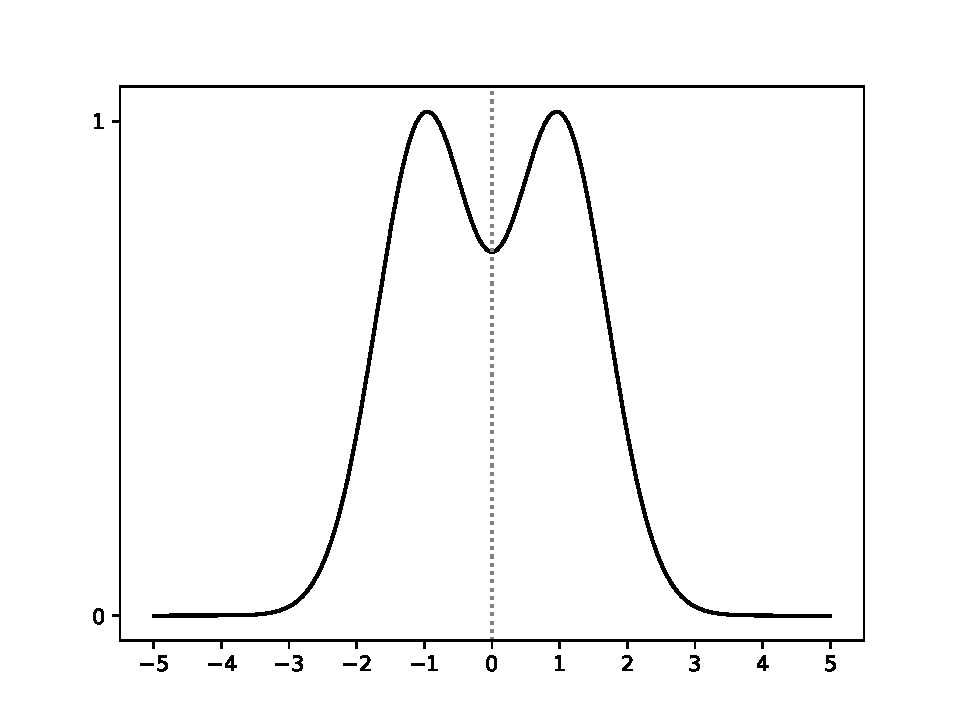
\includegraphics[width=0.6\textwidth]{pics/camel.pdf}
			\\  $f(x) = e^{-(x-1)^2} + e^{-(x+1)^2}$ erreicht ein lokales Minimum in $0$, aber kein globales Minimum; denn $f(0) = \frac{2}{e} >0$, während $f(x)$ für große $|x|$ beliebig klein positiv wird. 
		\end{center}
	
\end{bsp} 

\begin{bsp} 
	$f(x) = \arctan x$ erreicht weder lokales Minimum noch ein lokales Maximum. 
\end{bsp} 

\begin{defn}
	$C \in [-\infty,\infty]$ heißt \textbf{obere Schranke} an $f : X \to \R$, wenn $f(x) \le C$ für alle $x \in X$ gilt. $c \in [-\infty,\infty]$ heißt \textbf{untere Schranke} an $f : X \to
 \R$, wenn $f(x) \ge c$ für alle $x \in X$ gilt.  $f : X \to \R$ heißt nach oben bzw. unten \textbf{beschränkt}, wenn $f$ eine endliche obere bzw. untere Schranke hat. 
 
	Das \textbf{Supremum} von $f$ auf $X$ ist 
	\[
		\sup_{x \in X} f(x) \ :=  \ \text{die kleinste obere Schranke von $f : X \to \R$}
	\]
	Das \textbf{Infimum} von $f$ auf $X$ ist 
	\[
		\inf_{x \in X} f(x)  \ :=  \ \text{die größte untere Schranke von $f : X \to \R$}.
	\]
\end{defn} 


\begin{bsp}
	Bei einer $f$, die ein endliches Supremum bzw. Infimum hat, muss das Maximum bzw. Minimum im Allgemeinen nicht erreicht werden. Z.B.:
	\begin{align*}
		\sup_{x \in \R} \  \arctan x &  = +\frac{\pi}{2},  & & |\text{ Max. wird nicht erreicht, owohl das Sup. endlich ist}
\\		\inf_{x \in \R} \ \arctan x & = -\frac{\pi}{2} & & |\text{ Min. wird nicht erreicht, obwohl das Inf. endlich ist}
	\end{align*}
	
	
	Man beachte: $\arctan(x)$ ist sehr regelmäßig (beliebig oft differenzierbar). 
	
	Problem hier: unbeschränktes $\R$. 
\end{bsp} 

\begin{bsp}
		\begin{align*}
			\sup_{-1 < x < 1} (5 x + x^3) & = 6  & & |\text{ Max. wird nicht erreicht,}
\\			\inf_{-1 < x < 1} (5  x+ x^3) & = 4 & & |\text{ Min. wird nicht ereicht.} 
		\end{align*}
		
		Problem hier: das Interval $(-1,1)$ ist zwar beschränkt aber nicht abgeschlossen. 
\end{bsp} 

\begin{bsp} 
		Durch $\lfloor x \rfloor$ wird das Abrunden bezeichnet. 
		\begin{align*}
			\sup_{0 \le x \le 1}  (x - \lfloor x \rfloor ) & = 1 & & |\text{ Max. wird nicht erreicht}. 
		\end{align*} 
		
		Problem hier: zwar ist $[0,1]$ kompakt (d.h., beschränkt und abgeschlossen), ist die Funktion nicht stetig. 
		
		Bei stetigen Funktionen auf einer kompakten Menge garantiert der Satz von Weierstraß, dass das Maximum sowie das Minimum erreicht werden. 
\end{bsp} 

\begin{thm} Sei $f : X \to \R$ zweimal differenzierbare Funktion auf einer Teilmenge $X$ von $\R$ und sei $a$ ein innerer Punkt von $X$, in welchem $f'(a) = 0$ gilt. Dann gilt: 
	\begin{enuma} 
		\item Ist $f''(a) > 0$, dann erreicht $f$ in $a$ ein lokales Minimum. 
		\item Ist $f''(a) < 0$, dann erreicht $f$ in $a$ ein lokales Maximum. 
	\end{enuma} 
\end{thm} 

\begin{bem}
	Um die Unterscheidung zwischen $f'(a) =0, f''(a) <0$ und $f'(a) = 0, f''(a)>0$ zu merken, denken Sie an die beiden Funktionen $f(x) =\pm x^2$ und $a=0$. 
\end{bem} 

\begin{bem}
	Für $f(x) = e^x - x$, ist $x=0$ die einzige Stelle mit $f'(x)=0$. An dieser Stelle gilt $f''(x) > 0$. Das $f$ erreicht also in $0$ ein lokales Minimum. Man kann zeigen, dass $f$ in $0$ sogar das globale Minimum erreicht, denn
	\begin{align*}
		\lim_{x \to +\infty} f(x) & = +\infty, 
	\\	\lim_{x \to -\infty} f(x) & = + \infty,
	\end{align*} 
	woraus man sieht, dass bei einem genügend großen $|x|$ der Wert $f(x)$ größer als $f(0) = 1$ ist. 
\end{bem} 

\begin{bsp}
	Man kann nicht immer (in der Praxis so gut wie nie) Lösungen der Gleichung $f'(x) = 0$ in einer abgeschlossenen Form finden. In der Praxis nutzt man numerische Verfahren so eine Art Gleichungen annähernd zu lösen. 
\end{bsp} 

\section{Konvexität}

\begin{defn} 
	Eine Menge $X \subseteq \R^n$ nennt man \text{konvex}, wenn für alle $a,b \in X$ und $0 \le \lambda \le 1$ die Bedingung $(1-\lambda) a + \lambda b \in X$ erfüllt ist. Mit anderen Worten: mit je zwei Punkten in $X$ ist die Verbindungsstrecke dieser Punkte Teilemenge von $X$. 
\end{defn} 

\begin{bem} 
	Konvexe Teilemengen von $\R$, die nicht aus einem einzigen Punkt bestehen sind \textbf{Intervalle}. Intervalle können beschränkt oder unbeschränkt, offen, abgeschlossen oder halboffen sein. 
\end{bem} 


\begin{defn}
	Eine Funktion $f : X \to \R$ auf einer konvexen Teilmenge $X$ von $\R^n$ nennt man \textbf{konvex}, wenn für alle $a,b \in X$ und alle $0 \le \lambda \le 1$ die Ungleichung 
	\[
		f( (1-\lambda) a + \lambda b) \le (1-\lambda) f(a) + \lambda f(b)
	\]
	erfüllt ist. 
	
	Eine Funktion $f$ nennt man \textbf{konkav}, wenn die Funktion $-f$ konvex ist. 
\end{defn} 

\begin{thm} Für eine differenzierbare Funktion $f : I \to \R$  auf einem Intervall $I$ sind die folgenden Bedingungen äquivalent: 
	\begin{enumi}
		\item $f$ ist konvex,
		\item $f'$ ist monoton steigend. 
	\end{enumi}
\end{thm} 

\begin{thm} Für eine zweimal differenzierbare Funktion $f : I \to \R$ auf einem Intervall $I$ sind die folgenden Bedingungen äquivalent: 
	\begin{enumi} 
		\item $f$ ist konvex, 
		\item $f'' \ge 0$ auf $I$.
	\end{enumi} 
\end{thm} 

\section{Der Mittelwertsatz der Differentialrechnung} 

\begin{thm}
	Sei $f: [a,b] \to \R$ eine stetige Funktion auf einem Interval $[a,b]$ mit $a,b \in \R$ und $a<b$, die auf $(a,b)$ differenzierbar ist. Dann existiert ein $\xi \in (a,b)$ mit 
	\[
		f'(\xi) = \frac{f(b) - f(a)}{b-a}. 
	\]
\end{thm} 

\begin{bem}
	Der Satz ist eine weitere Berechtigung für die Approximation der Ableitung durch einen Quotienten.
\end{bem} 

\begin{bem} 
	Geometrische Intuition sieht man am Graphen der Funktion: Die Sekante zu Punkten $(a,f(a))$ und $(b,f(b))$ wird durch eine geeignete Verschiebung zu einer Tangente an einem der Punkte $(\xi,f(\xi))$ mit $\xi \in (a,b)$. 
\end{bem} 


\begin{bem} 
	Weitere Intuition: Die Strecke von der BTU Cottbus bis zu Berlin Zoo ist $140$ km lang. Wenn wir diese Strecke in $1{,}5$ h geschafft haben, dann war unsere Geschwindigkeit in mindestens einem Zeitpunkt unserer Fahrt 
	\[
		\frac{140 \ \text{km} }{1{,}5 \ \text{h}} = 93 \frac{1}{3} \ \frac{\text{km}}{\text{h}}.
	\] 
	Das ist unsere Durchschnittsgeschwindigkeit. Die Durschnittsgewschindigkeit wird mindestens ein mal erreicht. 
	
	Die Funktion in diesem Beispiel ist: Zurückgelegter Weg $f(x)$ (in km) zum Zeitpunkt $x$ (in h) mit $0 \le x \le 1{,}5$, und wir setzen $a=0$ und $b=1{,}5$. 
\end{bem} 

\begin{defn}
	Man sagt, $\xi \in \R$ liegt zwischen $a \in \R$ und $b \in \R$, wenn $a \le \xi \le b$ oder $b \le \xi \le a$ erfüllt ist. 
\end{defn} 


\begin{bem} 
	Wir betrachten eine differentierbare Funktion $f : I \to \R$ auf einem Intervall und fixieren ein $a$ aus dem inneren von $I$. 
	Machen wir das $b$ variabel, und bezeichen es als $x$. Dann ist das $\xi$ zwischen $a$ und $x$ abhängig von der Wahl von $x$, und wir bezeichnen es als $\xi_x$. Das vorige Theorem ergibt: 
	\begin{align*}
		f'(\xi_x)  & = \frac{f(x)-f(a)}{x-a}  & & |\ \Rightarrow 
		\\ f(x) & = f(a) + f'(\xi_x) (x-a) & & |\text{ Nach $f(x)$ aufgelöst} 
	\end{align*}
	Dies ist die Taylorentwicklung der Ordnung $0$. 
	Dies ist ein Spezialfall einer viel allgemeineren Formel, die wir in Kürze diskutieren werden. 
\end{bem} 

\chapter{Taylor- und Potenzreihen} 

\section{Taylor-Entwicklung und Taylor-Reihen} 

\begin{defn} 
	Eine \textbf{Funktionsreihe} ist eine Ausdruck der Form $\sum_{k=0}^\infty g_k(x)$, in dem die Glieder $g_0(x),g_1(x),g_2(x),\ldots$ der Reihe Funktionen in $x$ sind. 
	
	Die Funktionsreihen der Form $\sum_{k=0}^\infty a_k (x-c)^k$, die durch Konstanten $c$ und die Folge von Konstanten $a_0,a_1,a_2,\ldots$ gegeben sind,  nennt man \textbf{Potenzreihen}. Den Wert $c$ nennt man den \textbf{Entwicklungspunkt} der Potenzreihe. 
\end{defn} 


\begin{bsp} 
	Die geometrische Reihe mit einer variablen Basis $x$ ist eine Potenzreihe, für welche die Summe bekannt ist: 
	\[
		\sum_{k=0}^\infty x^k = \frac{1}{1-x}
	\]
	Diese Gleichung gilt für $|x| < 1$, das heißt, für $x$ im offenen Intervall $(-1,1)$. 

	\begin{center}
	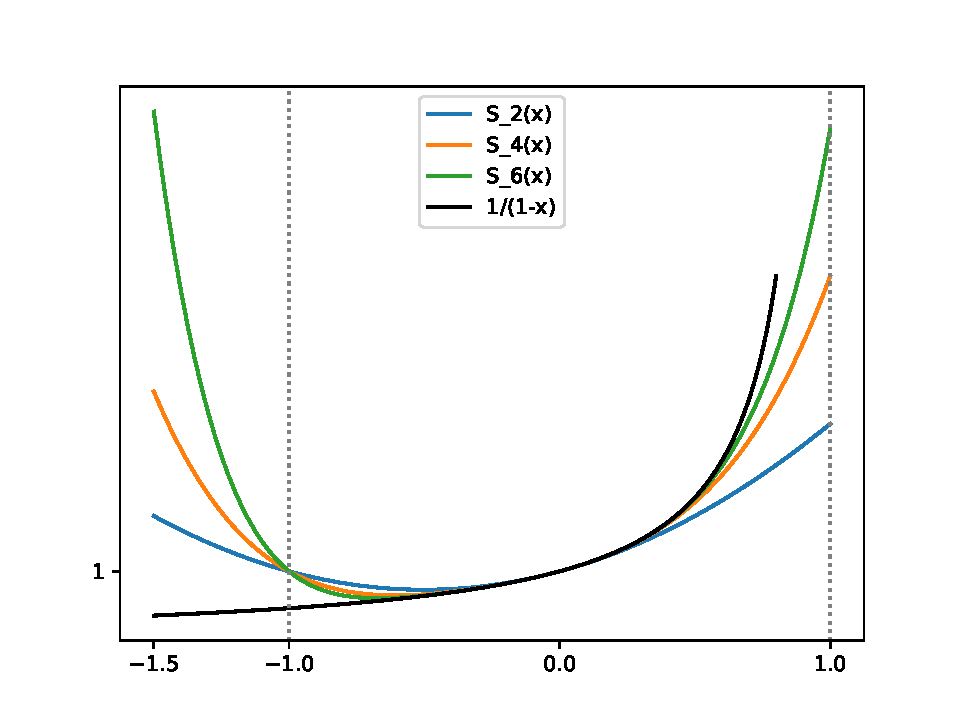
\includegraphics[width=0.6\textwidth]{pics/potenzreihe.pdf}
	\\ Partialsummen $s_n(x) := \sum_{k=0}^n x^k$.
	\end{center}
\end{bsp} 

\begin{bsp} Wir entwickeln die Funktion $\frac{1}{1+x^2}$ in die Potenzreihe zum Entwicklungspunkt $0$: 
	\begin{align*}
		\frac{1}{1+x^2} & = \sum_{k=0}^\infty (-x^2)^k & &|\text{ Formel für die Summe der Geom. Reihe}
		\\ & = \sum_{k=0}^\infty (-1)^k x^{2k} & &|\text{ Nur gerade Potenzen hier!} 
		\\ & = 1 - x^2 + x^4 - x^6 + \cdots & &| \text{ Potenzreihe mit den Koef.} \ 1, 0,-1,1,0,-1,\ldots 
	\end{align*}
	Man beachte: wir wissen aus der Analyse der geometrische Reihe, dass diese Entwicklung nur  für $x^2  < 1$, also für $|x| <1$, eine gültige Gleichung ergibt. Für $|x^2| \ge 1$, ist die Reihe divergent, auch wenn die Formel $\frac{1}{1+x^2}$, für die wir die Entwicklung aufstellen, für alle $x \in \R$ ausgewertet werden kann! 
	
	\begin{center}
	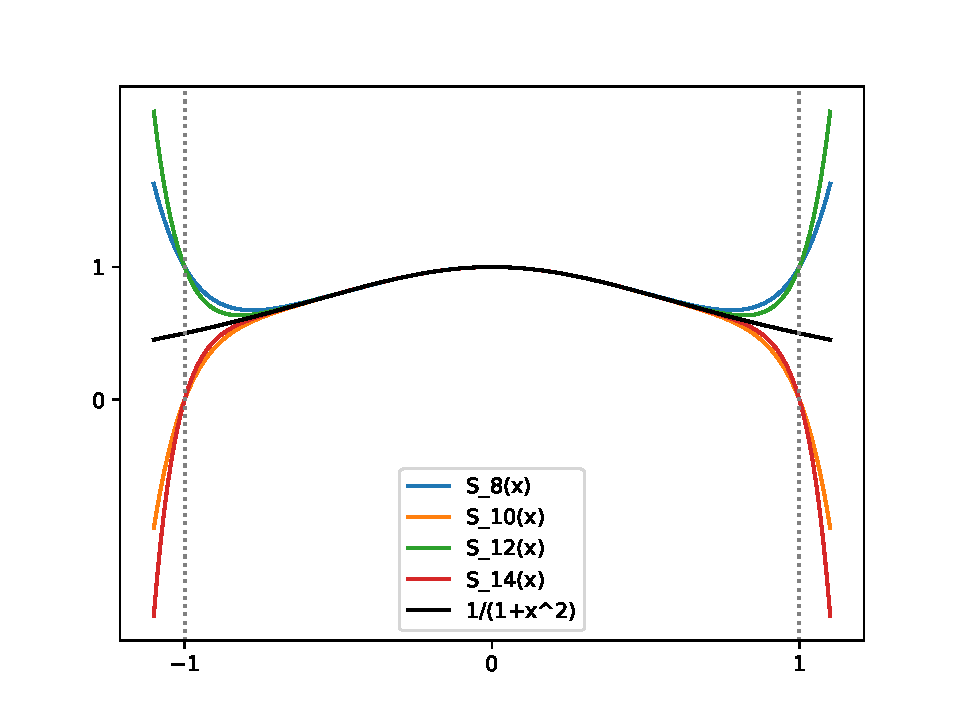
\includegraphics[width=0.6\textwidth]{pics/eins_durch_quadrat_plus_eins.pdf}
	\\ Partialsummen $s_n(x)$.
\end{center}

\end{bsp} 


\begin{defn} 
	Für eine Funktion $f : X \to \R$ auf $X \subseteq \R$, die an einer Stelle $a \in X$ $n$-mal differenzierbar ist, wird das \textbf{Taylor-Polynom} von $f$ der Ordnung $n$ bzgl. des Entwicklungspunkts $a$ durch 
	\[
		T_n(x) := \sum_{k=0}^n \frac{f^{(k)}(a)}{k!} (x-a)^k
	\]
	definiert. Die Funktion 
	\[
		R_n(x) := f(x) - T_n(x)
	\] nennt man das \textbf{Restglied} der Taylor-Entwicklung der Ordnung $n$ an der Stelle $a$. 
	
	Ist $f$ beliebig oft an der Stelle $a$ differenzierbar, so nennt man die Potenzreihe 
	\[
		T_\infty(x) := \sum_{k=0}^\infty \frac{f^{(k)}(a)}{k!} (x-a)^k
	\]
	die \textbf{Taylor-Reihe} von $f$ bzgl. des Entwicklungspunkts $a$. 
\end{defn} 

\begin{bem}[$T_n(x)$ aus einer anderen Perspektive]
	Was haben $f(x)$ das Polynom $T_n(x)$ gemeinsam? Die Ableitungen an der Stelle $a$. Wenn man die Ableitungen bis zur Ordnung $n$ von $T_n(x)$ ausrechnet, stellt man fest, dass sie mit den jeweiligen Ableitungen von $f$ übereinstimmen: 
	\begin{align} \label{T_n:bedingung} 
		T_n^{(i)}(a) & = f^{(i)}(a)  & & \text{für} \ i=0,\ldots,n.
	\end{align} 
	$T_n$ ist innerhalb von allen Polynomen vom Grad höchstens $n$ durch die Bedingung \eqref{T_n:bedingung} eindeutig bestimmt. 
\end{bem} 


\begin{bem}
	Wir werden feststellen, dass unter gewissen Voraussetzung der Unterschied zwischen $T_n(x)$ und $f(x)$ sehr klein ist, wenn $x$ nah am Entwicklungspunkt $a$ liegt. 
\end{bem} 

\begin{defn}[$O$-Notation  für $x\to a$]  
	Seien $f,g : X \to \R$ Funktionen auf $X \subseteq \R$ und $a$ Häufungspunkt von $X$. Man schreibt, 
	\[
		f(x) = O(g(x)), \qquad \text{für} \ x \to a,
	\] 
	und sagt dabei $f(x)$ hat die \textbf{Ordnung O} von $g(x)$ für $x \to a$ hat, 
	wenn eine Konstante $C\ge 0$ und ein $\delta > 0$ existieren, für welche die Ungleichung 
	\[
		|f(x)| \le C |g(x)| 
	\]
	für alle $x \in X$ mit $|x-a| < \delta$ erfüllt ist. 
		
	Formale Beschreibung: $f(x) = O(g(x))$ heißt
	\[
		\exists \, C \in \R_{\ge 0} \ \exists \, \delta \in \R_{>0} \ \forall \, x \in X \,:\, |x-a| < \delta \Rightarrow |f(x)| \le C |g(x)|.
	\]
\end{defn} 


\begin{bem}
	Sie kennen bestimmt verschiedene Formen der asymptotischen Notation für Funktionen  in einer Variablen $n$ aus $\N$ aus der Informatik, da diese Notation bei der Analyse der Laufzeit von Algorithmen sehr oft verwendet ist. All die Bezeichnungen, die man bei der Analyse der Laufzeit von Algorithmen benutzt, kann man auch für Funktionen in einer reellwertigen Variablen $x$ für $x \to a$ einführen. 
	
	Neben der O-Notation hat man zum Beispiel auch $\Omega$-, $\Theta$- und $o$-Notation für $x \to a$. Die Bedingung $f(x) = o(g(x))$ für $x \to a$ heißt zum Beispiel, dass 
	\[
		\lim_{x \to a} \frac{f(x)}{g(x)} = 0
	\]
	gilt. 
\end{bem} 

\begin{aufg}
	Finden Sie ein $p \in \R$ derart, dass $\sqrt{1+x} - \sqrt{1-x} = \Theta (x^p)$ für $x \to 0$ gilt. 
\end{aufg} 


\begin{defn}
	Eine Funktion $f: X \to \R$ auf $X \subseteq \R$ nennt man \textbf{$n$-mal stetig differenzierbar}, wenn die Ableitungen $f, f',\ldots, f^{(n)}$ stetige Funktionen auf $X$ sind. 
\end{defn} 

\begin{thm}[Über Approximation durch Taylor-Entwicklung]  
	Sei $f : I \to \R$ $(n+1)$-mal stetig differenzierbare Funktion auf einem Intervall $i$  und $a$ ein innerer Punkt von $I$. Dann gilt für das Restglied $R_n(x)$ der Taylor-Entwicklung  der Ordnung $n$ bzgl. $a$ die asymptotische Abschätzung
	\[
		R_n(x) = O( (x-a)^{n+1}), \qquad x \to a. 
	\]
	Mit anderen Worten: 
	\[
		f(x) = T_n(x) + O((x-a)^{n+1}), \qquad x \to a. 
	\]
\end{thm} 

\begin{bem}
	Interessante Spezialfälle sind die lineare Approximation
	\[
		f(x) = f(a)+ f'(a) (x-a) + O((x-a)^2), \qquad x \to a. 
	\]
	und die quadratische Approximation
	\[
		f(x) = f(a) + f'(a)(x-a) + \frac{1}{2} f''(x) (x-a) + O((x-a)^3), \qquad x \to a. 
	\]
	Die notwendigen und hinreichenden der Bedingungen der Optimalitität erhält man aus diesen Approximationen. 
\end{bem}


\begin{bem} 
	Das vorige Theorem ist Folgerung aus einem Theorem, welches etwas mehr Details über eine mögliche Darstellung des Restlieds verrät. 
\end{bem} 

\begin{thm}[Über die Darstellung des Restglieds] 
	Sei $f: I \to \R$ $(n+1)$-mal stetig differenzierbare Funktion auf einem Intervall $I$ und sei $a$ innerer Punkt von $I$. Man betrachte das Taylor-Polynom $T_n(x)$ von $f$ der $n$-ten Ordnung bzgl. des Entwicklungspunkts $a$. Dann existiert für jedes $x \in I$ ein $\xi_x \in I$, das zwischen $a$ und $x$ liegt, mit 
	\[
		f(x)  = T_n(x) + \frac{f^{(n+1)}(\xi_x)}{(n+1)!} (x-a)^{n+1}. 
	\]
	Insbesondere gilt 
	\[
		|f(x) - T_n(x)| \le \frac{M_{n+1}}{(n+1)!} |x-a|^{n+1},
	\]
	wenn $M_{n+1}$ eine Konstante ist, welche den Betrag der $(n+1)$-ten Ableitung auf dem Interval $I$ nach oben abschätzt. 
\end{thm} 

\begin{bsp}
	Wir approximieren $f(x)$ auf $x \in [-1,1]$ durch die Taylorentwicklung erster Ordnung im Punkt $0$ und schätzen die Qualität der Approximation ab: 
	\begin{align*}
		& f(x)  = f'(x) = e^x & & \Longrightarrow & & f(0)  = f'(0) = 1  \\ 
		& & & \Longrightarrow &  & T_1(x) = f(0) + f'(0) x = 1 + x. 
	\end{align*}
	Es gilt: 
	\begin{align*}
		| e^x - (1+x) | \le \frac{M_2}{2!} x^2 & & \text{für} -1 \le x \le 1
	\end{align*}
	mit 
	\[
		M_2 = \max_{-1 \le x \le 1} |f''(x)| = \max_{-1 \le x \le 1} | e^x | = e.
	\]
	Fazit: 
	\begin{align*}
		|e^x - (1+x)| \le \frac{e}{2} \cdot x^2 & & \text{für} \ -1 \le x \le 1.
	\end{align*}
\end{bsp} 

\begin{bsp} 
	Wir approximieren $f(x) = \sin x$ auf $x \in [-\pi/2,\pi/2]$ durch die Taylorentwicklung zweiter Ordnung im Punkt $0$ und schätzen die Qualität der Approximation ab. 
	\[
		\begin{array}{|ccc|c|ccc|cccc}
		f(x) & = & \sin x &  &  f(0) & = & 0 & \\ 
		f'(x)  & = & \cos x & \Longrightarrow & f'(0) & =   & 1 & \Longrightarrow & T_2(x) &  = & x. \\ 
		f''(x)  & =  & - \sin x &  &  f''(0) & = & 0 &
		\end{array} 
	\]
	Es gilt
	\[
		|x - \sin x| \le \frac{M_3}{3!} |x|^3
	\]
	mit 
	\[
		M_3 = \max_{-\pi/2 \le x \le \pi/ 2} | f'''(x) | = \max_{-\pi/2 \le x \le \pi / 2} | - \cos x| = 1.
	\]
	Fazit: 
	\begin{align*}
			|x - \sin x| & \le \frac{1}{6} |x|^3 & & \text{für} \ -\pi/2 \le x \le \pi/2. 
	\end{align*}
\end{bsp} 

\begin{aufg}
	Rechnen Sie $T_\infty(x)$ bzgl. der Entwicklungsstelle $a=0$ für die  Funktionen $e^x, \cos x, \sin x$ und $\frac{1}{1-x}$ aus: 
\end{aufg} 

\begin{aufg}
	Rechnen Sie $T_\infty(x)$ bzgl. der Entwicklungsstelle $a=0$ für $\ln x$ aus. 
\end{aufg} 

%\begin{bem}
%	Ein isolierter Punkt der Menge hält einen Mindestabstand zu allen anderen Punkten der Menge: Nicht unbedingt $1{,}5$ Meter, aber zumindest ein festes $\epsilon>0$. 
%\end{bem} 

%\begin{bsp}
%	\begin{enuma} 
%		\item alle Punkte von $\Z$ sind isoliert (Mindestabstand $1/2$). 
%		\item $\setcond{\frac{1}{n}}{n \in \N}$
%	\end{enuma} 
%\end{bsp} 

\section{Potenzreihen} 

\begin{defn} 
	$C \in [-\infty,\infty]$ heißt obere Schranke an eine Menge $X \subseteq \R$ wenn $x \le C$ für alle $x \in X$ erfüllt ist.
	
	$c \in [-\infty,\infty]$ heißt untere Schranke an eine Menge $X \subseteq \R$, wenn $x \ge c$ für alle $x \in A$ erfüllt ist. 
	
	Wir definieren das Supremum/Infimum einer Menge $X$ als:
	\begin{align*}
		\sup X & :=  \ \text{kleinste obere Schranke an $X$},
	\\	\inf X  & := \ \text{größte untere Schranke an $X$}
	\end{align*}
\end{defn} 

\begin{bsp}
	Supremum und Infimum für $\R$, leere Menge und das offene Intervall $(0,1)$. 
	\begin{align*}
		\sup \R & = + \infty  &  \sup \emptyset & = - \infty & \sup (0,1) & = 1
		\\ \inf \R & = -\infty & \inf \emptyset & = +\infty & \inf (0,1)  & = 0. 
	\end{align*}
\end{bsp} 

\begin{defn}
	Für die Potenzreihe $\sum_{k=0}^\infty a_k (x-c)^k$ nennt man die Menge 
	\[
		 X:= \setcond{x \in \R}{\sum_{k=0}^\infty a_k (x-c)^k \ \text{konvergent}} 
	\]
	den \textbf{Konvergenzbereich} der Reihe und den Wert 
	\[
		\rho := \sup \setcond{|x-c|}{x \in X}
	\]
	den \textbf{Konvergenzradius}. 
\end{defn} 


\begin{bem}
	Der Konvergenzradius ist ein Wert $\rho \in [0,\infty]$. Wenn man $\rho=0$ hat, dann konvergiert die Reihe nur für $x=c$. 
\end{bem} 

\begin{bsp}
	Für $\sum_{k=0}^\infty x^k$ ist der Konvergenzbereich $X = (-1,1)$ und somit der Konvergenzradius $\rho = \sup \setcond{|x|}{x \in X} = 1$.  

	Hier ein Bild mit den Graphen der Logarithmen der Partialsummen $\sum_{k=0}^n x^k$ für einige $n$ im Bereich von $100$ bis $200$: 
 \begin{center} 	
			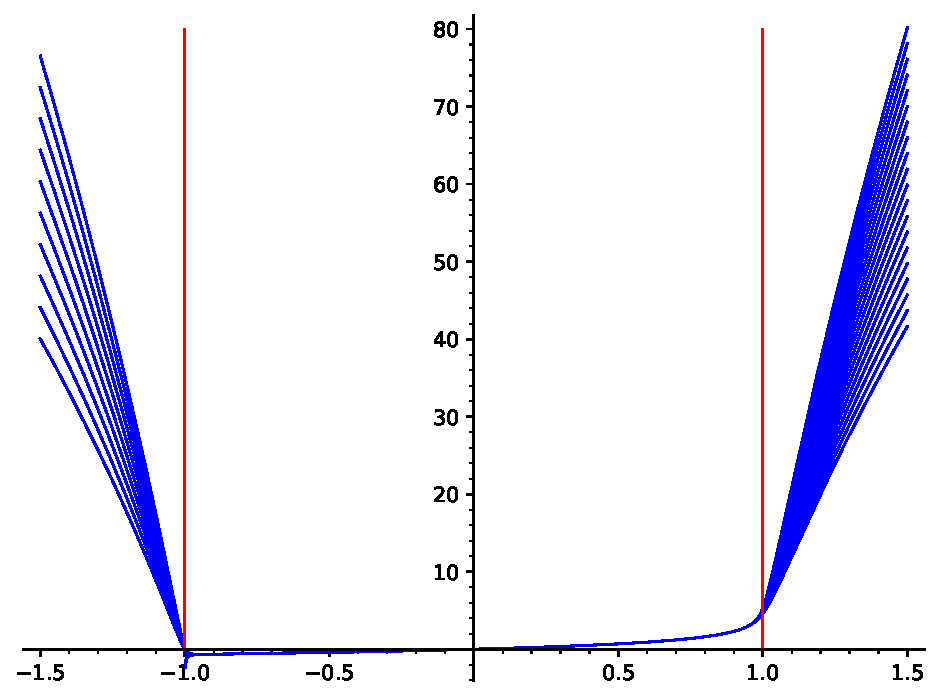
\includegraphics[width=0.5\textwidth]{pics/konvergenzradius_potenzreihe.pdf}
	\end{center} 
	Wie man sieht, kommt es bei der Entfernung $1$ vom Entwicklungspunkt zu einer Art Explosion  - es findet der Übergang von Konvergenz zur Nicht-Konvergenz statt. Der Logarithmus  wurde  genommen, um die Explosion graphisch darstellen zu können (sonst wäre das Wachstum der Funktionen zu schnell). 
	
	Im Folgenden Theorem wir behauptet, dass jeder Konvergenzbereich ein Intervall ist, das $c$ genau in der Mitte hat...
\end{bsp} 

\begin{thm}
	Für die Potenzreihe $\sum_{k=0}^\infty a_k (x-c)^k$ mit dem Konvergenzradius $\rho$ gilt: 
	\begin{enuma}
		\item Die Reihe ist absolut konvergent für alle $x \in \R$ mit $|x-c| < \rho$
		\item Die Reihe ist divergent für alle $x \in \R$ mit $|x-c| > \rho$.
		\item Im Fall $0 < \rho < \infty$ kann man über die Konvergenz in den beiden Punkten $x \in \R$ mit $|x-c| = \rho$ a priori nichts sagen: das heißt, der Konvergenzbereich ist $[c-\rho,c+\rho]$ oder $(c-\rho,c+\rho]$ oder $[c-\rho,c+\rho)$ oder $(c-\rho,c+\rho)$ und im Allgemeinen ist jeder dieser vier Fälle möglich. 
	\end{enuma}
\end{thm} 

\begin{bsp} 
	Die Potenzreihe $\sum_{k=0}^\infty \frac{(-1)^k}{k} x^k$ hat den Konvergenzbereich $(-1,1]$.  
	
	Begründung: 
	\begin{enuma}
		\item Für $|x| > 1$, ist das Glied der Reihe keine Nullfolge, sodass die Reihe für diese Wahl von $x$ nicht konvergent ist. 
		\item Für $-1 < x < 1$ folgt die Konvergenz aus dem Quotientenkriterium. 
		\item Für $x=1$ folgt die Konvergenz aus dem Leibniz-Kriterium. 
		\item Für $x=-1$ ist das die harmonische Reihe und somit eine divergente Reihe. 
	\end{enuma} 
\end{bsp} 

\begin{bsp} 
	Wie kann man den Konvergenzbereich bzw. -radius von $\sum_{k=0}^\infty 2^{-k} x^k$ ohne (komplizierte) Hilfsmittel berechnen? 
	
	
	Wir wissen: die geometrische Reihe $\sum_{k=0}^\infty x^k$ konvergiert genau dann, wenn $|x| < 1$ gilt. 
	
	Es folgt: 
	\[
		\sum_{k=0}^\infty 2^{-k} x^k = \sum_{k=0}^\infty \left( \frac{x}{2}\right)^k
	\]
	konvergiert genau dann wenn $\left| \frac{x}{2} \right|  < 1$ gilt. 

	Fazit: Konvergenzradius von $\sum_{k=0}^k 2^{-k} x^k$ ist $2$. 
\end{bsp} 

\begin{bem} 
	Wie kann man das vorige Beispiel auf allgemeinere Potenzreihen $\sum_{k=0}^\infty a_k (x-c)^k$ verallgemeinern? Betrachten wir Einfachheit halber den Fall $a_k > 0$. 
	
	Man hat 
	\[
		 a_k (x-c)^k   = \left( a_k^{1/k} (x-c) \right)^k
	\] 
	
	Das heißt: Wenn $a_k^{1/k}$ einen Grenzwert $\gamma$ besitzt, so verhält sich $a_k (x-c)^k$ ungefähr wie der $k$-te Term der geometrischen Reihe mit der Basis $\gamma (x-c)$. Für die Geometrische $\sum_{k=0}^\infty (\gamma (x-c))^k$ hat man aber die Konvergenz genau dann, wenn $|\gamma (x-c)| < 1$ erfüllt ist, sodass ihr Konvergenzradius gleich $\frac{1}{\gamma}$ ist. 
	
	Dies ist die Intuition hinter dem folgenden Theorem...
\end{bem} 

\begin{thm}
	Wenn die Potenzreihe $\sum_{k=0}^\infty a_k (x-c)^k$ einen Grenzwert $\lim_{k \to \infty} |a_k|^{1/k} \in [0,+\infty]$ besitzt ($0$ und $+\infty$ sind beide zugelassen), dann ist der Konvergenzradius der Reihe gleich 
	\begin{align}
		\label{konv:rad:wurzel:lim}
		\rho = \frac{1}{ \lim_{k \to \infty} |a_k|^{1/k}},
	\end{align}
	wobei man $1/0$ bzw. $1/\infty$ auf der rechten Seite von \eqref{konv:rad:wurzel:lim} als $\infty$ bzw. $0$ interpretiert. 
\end{thm} 

\begin{bsp} 
	Für $\sum_{k=0}^\infty (2+ 1/k)^k x^k$ gilt 
	\[
		\lim_{k \to \infty} (( 2 + 1/k)^k)^{1/k} = \lim_{k \to \infty} (2 + 1/k)  = 2. 
	\]
	Der Konvergenzardius der Reihe ist $ 1/2$. 
\end{bsp} 

\begin{bsp} 
	Der Konvergenzradius von $\sum_{k=0}^\infty k^k x^k$ ist $0$. Das heißt, die Reihe konvergiert nur für $x=0$. 
\end{bsp} 

\begin{bsp} 
	Der Konvergenzardius von $\sum_{k=0}^\infty k^{-k} x^k$ ist $\infty$. Das heißt, die Reihe konvergiert (absolut) für alle $x$. 
\end{bsp} 

\begin{bem} 
	Das vorige Theorem ist für die Beispiele wie z.B.
	\[
		\sum_{t=0}^\infty x^{t^2} = 1 + x + x^4 + x^9 + x^{16} + \cdots 
	\]
	nicht anwendbar, da hier die Folge $a_k^{1/k}$ keinen Grenzwert hat. Es gibt abere eine allgemeinere Version des Theorems. 
\end{bem} 

\begin{defn} 
	Für eine Folge $(x_k)_{k \in \N_0}$ ist der \textbf{Limes Superior}
	\[
		\limsup_{k \to \infty} x_k := \text{der maximale Grenzwert einer konvergenten Teilfolge von} \ (x_k)_{k \in \N_0}.
	\]
	wenn die Folge nach oben beschränkt ist, und
	$\limsup_{k \to \infty} x_k = \infty$, wenn die Folge nach oben unbeschränkt ist. 
\end{defn}

\begin{bem}
	Sind alle $x_k$ nicht negativ, und die Teilfolge aus den positiven Gliedern konvergent, dann gilt 
	\[
		\limsup_{k \to \infty} x_k = \text{der Grenzwert der Teilfolge der positiven Glieder von} \ (x_k)_{k \in \N_0}.  
	\]
\end{bem} 

\begin{thm}[Update]
	Der Konvergenzradius der Potenzreihe $\sum_{k=0}^\infty a_k (x-c)^k$ ist
	\begin{align}
		\label{eq:konv:rad:limsup}
	\rho = \frac{1}{ \limsup_{k \to \infty} |a_k|^{1/k}},
	\end{align}
	wobei man $1/0$ bzw. $1/\infty$ auf der rechten Seite von \eqref{eq:konv:rad:limsup} als $\infty$ bzw. $0$ interpretiert. 
\end{thm} 

\begin{bsp} 
	Der Konvergenzradius von $\sum_{t=0}^\infty x^{t^2}$ ist $1$, da der Limes Superior der Folge 
	\[
		a_k = \begin{cases}
			1 & k=t^2  \ \text{für ein $t \in \N_0$}
			\\ 0 & \ \text{sonst}
		\end{cases} 
	\]
	gleich $1$ ist. 
\end{bsp} 

\begin{bem}
	Es gibt eine weitere nützliche Formel für den Konvergenzradius im Fall, dass man $a_k=0$ nur für endlich viele $k \in \N_0$ hat. Die Formel ergibt als direkte Folgerung aus dem Quotientenkriterium (in der Grenzwert-Form) für Reihen...
\end{bem} 

\begin{thm} 
	Sei $\sum_{k=0}^\infty a_k (x-c)^k$ Potenzreihe, in der $a_k=0$ nur für endlich viele $k \in \N_0$ erfüllt ist und für welche der Grenzwert 
	\[
		\rho:=\lim_{k \to \infty} \left| \frac{a_k}{a_{k+1}} \right| 
	\] als Wert aus $[0,\infty]$ existiert. Dann ist  $\rho$ der Konvergenzradius dieser Potenzreihe. 
\end{thm} 

\begin{bsp} 
	Der Konvergenzradius von $\sum_{k=0}^\infty \frac{1}{k!} x^k$ ist $\infty$. 
\end{bsp} 

\begin{bsp} 
	Der Konvergenzradius von $\sum_{k=1}^\infty \frac{(-1)^k}{k} x^k$ ist $1$. 
\end{bsp} 

\begin{thm}
	Sei $\sum_{k=0}^\infty a_k (x-c)^k$ Potenzreihe und sei Konvergenzradius $\rho$ dieser Reihe ungleich $0$, d.h., $\rho \in (0,\infty]$. Dann ist $g(x) = \sum_{k=0}^\infty a_k (x-c)^k$ im Bereich $(c-\rho,c+\rho)$ beliebig oft differenzierbar. Darüber hinaus gilt:  
	\begin{itemize} 
	\item Die	$i$-te Ableitung $g^{(i)} (x)$ mit $i \in \N$ lässt als eine Potenzreihe durch gliederweises Differenzieren der Reihe $\sum_{k=0}^\infty a_k (x-c)^k$ darstellen. Das heißt, die Reihe $\sum_{k=0}^\infty ( a_k (x-c)^k)^{(i)}$ ist absolut konvergent in $(-\rho + c,c+\rho)$ mit
	\[
		g^{(i)}( x) = \sum_{k=0}^\infty \bigl( a_k (x-c)^k \bigr)^{(i)}.
	\]
	\item Man hat $a_k = \frac{g^{(k)}(c)}{k!}$ für alle $k \in \N$. 
	\end{itemize} 
\end{thm} 


\begin{bem}
	Das vorige Theorem zeigt: jede Potenzreihe (mit einem positiven Konvergenzradius) ist eine Taylorreihe einer unendlich oft differenzierbaren Funktion. 
\end{bem} 

\begin{bsp}
	Die Berechnung in diesem Beispiel machen wir für $x \in (-1,1)$. 
	Wir wissen, dass 
	\[
		\frac{1}{1-x} = \sum_{k=0}^\infty x^k
	\]
	gilt. Nach dem vorigen Theorem können wir diese Gleichung differenzieren, indem wir die Glieder der Reihe auf der rechten Seite differenzieren. Wir erhalten also 
	\[
		\frac{1}{(1-x)^2} = \left( \frac{1}{1-x} \right)' =  \sum_{k=0}^\infty (x^k)' = \sum_{k=1}^\infty k x^{k-1}. 
	\]
	Die Formel
	\[
		\frac{1}{(1-x)^2} = \sum_{k=1}^\infty k x^{k-1}
	\]
	kann man auch mit der Verwendung des Cauchy-Produkts erhalten. Wenn wir noch einmal differenzieren, erhalten wir 
	\[
		\frac{2}{(1-x)^3} =\sum_{k=2}^\infty k (k-1) x^{k-2}. 
	\]
	Diese Gleichung kann man auch als 
	\[
		\frac{1}{(1-x)^3} = \sum_{k=2}^\infty \binom{k}{2} x^{k-2} 
	\]
	mit Hilfe von Binomialkoeffizienten umschreiben. 
\end{bsp} 

\begin{aufg} 
	Finden Sie eine Darstellung von $(1-x)^{-d}$ mit $d \in \N$ und $-1 < x < 1$ als eine Potenzreihe in $x$, indem Sie die Darstellung von $\frac{1}{1-x}$ als Summe der geometrischen Reihe gliederweise $(d-1)$-mal differenzieren. 
\end{aufg} 

\begin{defn} 
	Eine Funktion $g$ heißt \textbf{analytisch} in $X$, wenn man für jedes $c \in X$ ein $\epsilon>0$ und eine Potenzreihe $\sum_{k=0}^\infty a_k (x-c)^k$ mit dem Konvergenzradius $> \epsilon$ findet, für welche die Gleichung
	\[	
			g(x) = \sum_{k=0}^\infty a_k (x-c)^k 
	\]
	für alle $x \in (c-\epsilon, c+ \epsilon)$ erfüllt ist. 
\end{defn} 

\begin{thm} 
	Ist $g$ analytisch in $X$, dann ist $g$ beliebig oft differenzierbar in $X$. 
\end{thm} 

\begin{bem} 
	Die Umkehrung gilt im Allgemeinen nicht. Die Funktion
	\[
		f(x) := \begin{cases} 
			e^{-1/x} & \ \text{für} \ x >0,
			\\ 0 & \ \text{für}  \ x \le 0
		\end{cases} 
	\]
	ist beliebig oft differenzierbar auf $\R$, ist aber nicht analytisch (Problemstelle ist die $0$). 
	
	Für diese Funktion hat man $f^{(k)}(0)$ für alle $k \in \N_0$. Das heißt: die Taylorreihe $T_\infty(x)$ dieser Funktion zum Entwicklungspunkt $0$ definiert eine Funktion, die identisch gleich $0$ ist, obwohl die Funktion $f$ in keiner Umgebung von $0$ identisch null ist. 
\end{bem} 

\begin{thm}
	$e^x, \sin x, \cos x, \ln x$, Polynome $p(x)$ und die Quotienten $p(x)/q(x)$ von Polynomen sind analytische Funktionen in ihren natürlichen Definitionsbereichen. 
\end{thm}

\begin{thm} 
	Man hat 
	\begin{align*}
		e^x & = \sum_{k=0}^\infty \frac{1}{k!} x^k,
		\\ \cos x & = \sum_{k=0}^\infty \frac{(-1)^k}{(2k)!} x^{2k},
		\\ \sin x & = \sum_{k=0}^\infty \frac{(-1)^k}{ (2k +1)!} x^{2k+1}
	\end{align*} 
	für alle $x \in \R$ und 
	\begin{align*}
		\ln (1+x) & = \sum_{k=1}^\infty \frac{(-1)^k}{k} x^k
	\end{align*}
	für alle $x \in (-1,1)$. 
\end{thm} 

\begin{bem} 
	Die vorigen Formeln werden aus der Abschätzung des Restgliedes hergeleitet. Zum Beispiel: für $f(x) = \sin x$ hat man 
	\[
		| \sin x - T_n(x) | \le \frac{ M_{n+1}}{(n+1)!} |x|^{n+1}
	\]
	mit 
	\[
		M_{n+1} \le \max_{x \in \R} |f^{(n+1)}(x)| \le 1,
	\]
	denn $f^{(n+1)}(x)$ ist $\pm \sin x$ oder $\pm \cos x$. 
	Es folgt: 
	\[
		| \sin x - T_n(x) | \le \frac{|x|^{n+1}}{(n+1)!}. 
	\]
	Wegen $\lim_{n \to \infty} \frac{|x|^{n+1}}{(n+1)!} = 0$, erhält man 
	\[
		| \sin x - T_\infty(x)| = 0. 
	\]
\end{bem} 

\begin{aufg}
	Verifizieren Sie analog die angeführten Darstellungen als Reihe für $e^x, \cos x$ und $\ln (1+x)$. 
\end{aufg} 

\begin{bem} 
		Potenzreihen für Quotienten von Polynomen kann man mit Hilfe von Ableitungen (als Taylorreihen) aber auch elementar ausrechnen...
\end{bem} 

\begin{bsp} 
Wir entwickeln $\frac{1}{x^2 - 5 x + 6}$ in eine Potenzreihe bzgl. des Entwicklungspunkts $0$ auf eine elementare Weise, mit der Verwendung der Formeln für die Summe der geometrischen Reihe: 
	
	\begin{align*} 
			\frac{1}{x^2 - 5 x + 6}  & 
			= \frac{1}{ (2-x) (3-x) }  
			\\ & = \frac{1}{2-x} - \frac{1}{3-x} 
			\\ & = \frac{1}{2} \cdot \frac{1}{1 - x/2} - \frac{1}{3} \cdot \frac{1}{1- x/3} 
			\\ & = \frac{1}{2} \sum_{k=0}^\infty (x/2)^k - \frac{1}{3} \sum_{k=0}^\infty (x/3)^k
			\\ & = \sum_{k=0}^\infty (2^{-k-1} - 3^{-k-1}) x^k. 
	\end{align*}
	Die Gleichung 
	\[
		\frac{1}{x^2 - 5 x + 6} = \sum_{k=0}^\infty (2^{-k-1} - 3^{-k-1}) x^k
	\]
	gilt für $x \in (-2,2)$. 
\end{bsp} 

\section{Exkurs in komplexwertige  Funktionen} 

\begin{bem} 
	Potenzreihen und analytische Funktionen können analog bzgl. komplexer Zahlen eingeführt werden. Die Menge der komplexen Zahlen ist ein ``natürlicher Lebensraum'' für Potenzreihen und analytische Funktionen. 
\end{bem} 

\begin{bsp} 
	$\frac{1}{1+ x^2}$ hat Konvergenzradius $1$, auch wenn diese Funktion auf dem gesamten $\R$ definiert und beliebig oft differenzierbar ist. Was ist der Grund? Wir erweitern diese Funktion auf die Menge der komplexen Zahlen.
	
	Die Funktion $f(z): = \frac{1}{1+z^2}$ hat die Entwicklung 
	\[
		f(z) = \sum_{k=0}^\infty (-1)^k z^{2 k}
	\]
	für alle $z \in \C$ mit $|z| < 1$.  Die komplexen Polstellen $z = \pm \iu$ mit $|z|=1$ sind Nachweis dafür, dass der Konvergenzradius nicht größer als $1$ sein kann. 
	
	\begin{center} 
		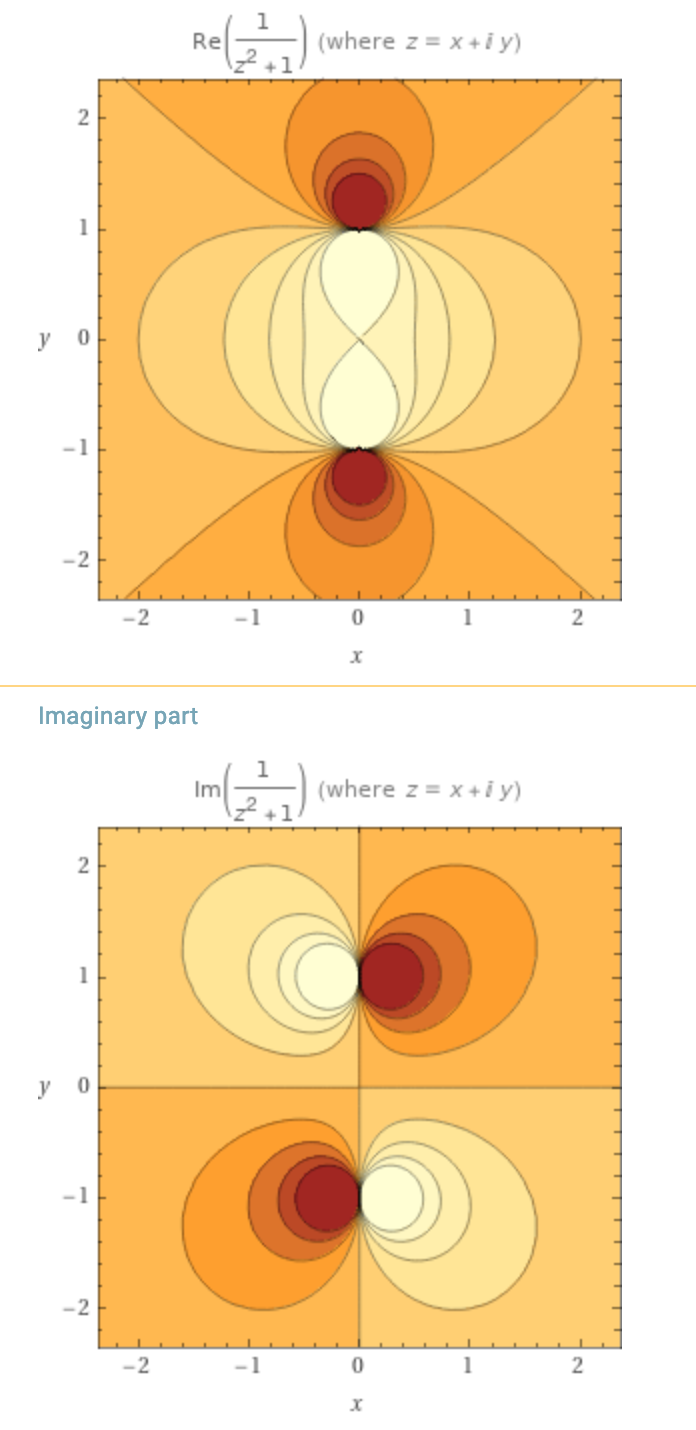
\includegraphics[width=0.3\textwidth]{pics/WolframComplexPlot.png}
	\end{center} 
\end{bsp} 

\begin{bem}
	$\cos z, \sin z, e^z$ können durch entsprechende Reihen für alle $z \in \C$ definiert werden. Man erhält:  
	\begin{align*}
		e^{\iu z} & = \sum_{k=0}^\infty \frac{ (\iu z)^k }{k!} 
					\\ & =\sum_{k=0}^\infty \frac{ (\iu z)^{2 k} }{(2 k)!}  + \sum_{k=0}^\infty \frac{ (\iu z)^{2 k +1} }{(2 k+1)!} 
					\\ & = \sum_{k=0}^\infty \frac{ (-1)^k z^{2 k} }{(2 k)!}
					 + \iu \sum_{k=0}^\infty \frac{(-1)^k z^{2 k +1}}{(2k+1)!}
					 \\ & = \cos z + \iu \sin z. 
	\end{align*}
	Wir erhalten also die sogenannte Eulersche Formel:
	\[
		e^{\iu z} = \cos z + \iu \sin z. 
	\]
\end{bem} 

\begin{bem} 
	Durch Eulersche Formel kann Trigonometrie durch Algebra ersetzt werden. 
	Wenn wir die Eulersche Formel zweimal benutzen
	\begin{align*}
		e^{\iu z} & = \cos z + \iu \sin z,
		\\ e^{-\iu z} & = \cos z - \iu \sin z 
	\end{align*}
	und dann die beiden Gleichungen nach $\cos z$ und $\sin z$ auflösen,  bekommen wir die Darstellung von $\cos z$ und $\sin z$ als 
	\begin{align*}
		\cos z & = \frac{ e^{\iu z} + e^{-\iu z}}{2},
	\\	\sin z & = \frac{ e^{\iu z} - e^{-\iu z}}{2 \iu}
	\end{align*}
\end{bem} 

\begin{bsp}
	Was heißt oben ``durch Algebra ersetzen''? Das heißt: trigonometrische Identitäten lassen sich aus den Algebraischen Identitäten herleiten. Nehmen wir die Formel 
	 \[
	 	\cos  2 \alpha  = \cos^2 \alpha - \sin^2 \alpha. 
	 \]
	 für den Kosinus des doppelten Winkel als ein Beispiel. Um diese Gleichung mit Hilfe der Euler-Formel algebraisch zu verifizieren, schreiben wir diese Gleichung als
	 \[
	 	 \frac{e^{\iu 2 \alpha} + e^{-\iu 2 \alpha}}{2} = \left( \frac{ e^{\iu \alpha}  + e^{-\iu \alpha}}{2} \right)^2 - \left( \frac{ e^{\iu \alpha}  -  e^{-\iu \alpha}}{2 \iu} \right)^2.
	 \]
	 um.  Die vorige Gleichung  kann mit Hilfe von $u := e^{\iu \alpha}$ als die algebraische Gleichung 
	 \[
	 	\frac{u^2 + u^{-2}}{2} = \left( \frac{u+ u^{-1}}{2}\right)^2 - \left( \frac{u -  u^{-1}}{2}\right)^2.
	 \]
	 formuliert werden. Dass die Gleichung in $u$ gilt, sieht man durch das Ausmultiplizieren der beiden Quadrate (mit der Verwendung der binomischen Formeln) auf der rechten Seite. 
\end{bsp} 

\begin{bsp}[Herleitung von Pythagoras]
	\begin{align*}
		1 & = e^0
		\\ & = e^{\iu z} e^{-\iu z} 
		\\ & = (\cos z + \iu \sin z) (\cos z - \iu \sin z) & &| \text{ nach der Euler-Formel}
		\\ & = \cos^2 z - (\iu \sin z)^2 & &| \text{ nach der dritten binomischen Formel}
		\\ & = \cos^2 z + \sin^2 z & &| \text{ wegen} \ \iu^2 = -1. 
	\end{align*}
\end{bsp} 

\begin{aufg} 
	Finden Sie ein einfache Formel für die Summe
	\[
		\sum_{k=0}^n \cos k \alpha
	\]
\end{aufg} 

\chapter{Integralrechnung I} 

\section{Riemann-Integral} 


\begin{defn} 
	Für $a, b \in \R$ mit $a<b$ nennt man eine endliche Teilmenge $Z$ mit \[
		\{a,b\} \subseteq Z \subseteq [a,b]
	\] eine \textbf{Zerlegung} von $[a,b]$. 
	
	Mit anderen Worten: Zerlegung eines abgeschlossenen Intervalls ist eine endliche Teilmenge des Intervalls, welche die beiden Endpunkte des Intervalls enthält. 
\end{defn} 


\begin{defn}
	Eine Zerlegung $Z = \{x_0,\ldots, x_n\}$ von $[a,b]$ aus $n+1$ Elementen mit $a = x_0 < x_1 < \cdots < x_n = b$ ergibt eine Darstellung von $[a,b]$ als Vereinigung der $n$ Intervalle $[x_{i-1},x_i]$ mit $i \in \{1,\ldots, n\}$.
	
 	Wir definieren für eine Funktion $f: [a,b] \to \R$ die \textbf{Unter-} und \textbf{Obersumme} von $f$ bzgl. $Z$ durch die Gleichungen: 
 	\begin{align*}
 		U_f(Z) & := \sum_{i=1}^n  \inf \setcond{f(x)}{x \in [x_{i-1},x_i]} \cdot (x_i - x_{i-1})
 		\\ O_f(Z) & := \sum_{i=1}^n \sup \setcond{f(x)}{x \in [x_{i-1},x_i]} \cdot (x_i - x_{i-1}).
 	\end{align*}  
 	In jeder der beiden Summe hat man einen Term pro jedes der $n$ Intervalle. 
\end{defn} 

\begin{defn}
	Direkt aus der Definition sieht man, dass $U_f(Z) \le O_f(Z)$ für alle Zerlegungen $Z$ von $[a,b]$ erfüllt ist. 
\end{defn} 

\begin{bem}[Verfeinerung] 
		Für eine Funktion $f : [a,b] \to \R$ und Zerlegungen $Z_1, Z_2$ von $[a,b]$ gilt: 
		\begin{align*}
			Z_1 & \subseteq Z_2 & & \Longrightarrow & U_f(Z_1) & \le U_f(Z_2)
			\\ Z_1 & \subseteq Z_2 & & \Longrightarrow & O_f(Z_1) & \ge O_f(Z_2)
		\end{align*} 
		
		Das heißt: 
		\begin{enuma} 
			\item Je feiner Zerlegung, desto größer die Untersumme. 
			\item Je feiner Zerlegung, desto kleiner die Obersumme. 
		\end{enuma} 
\end{bem} 

\begin{bem}
	Nehmen wir zwei Zerlegungen $Z_1, Z_2$, die nicht unbedingt kompatibel sind, d.h., weder $Z_1 \subseteq Z_2$ noch $Z_2 \subseteq Z_1$ ist vorausgesetzt. Dann ist die Zerlegung $Z_1 \cup Z_2$ feiner als $Z_1$ und $Z_2$ also erhalten wir 
	\[
		U_f(Z_1) \le U_f(Z_1 \cup Z_2) \le O_f(Z_1 \cup Z_2) \le O_f(Z_2). 
	\]
	Das zeigt
	\[
		U_f(Z_1) \le O_f(Z_2). 
	\]
	Also: jede beliebige Untersumme ist nicht höher als jede beliebige Untersumme. 
\end{bem} 

\begin{defn} 
	Wir definieren das \textbf{Riemannsche Unter-} bzw. \textbf{Oberintegral} als 
	\begin{align*}
		U_f & := \sup \setcond{ U_f(Z) }{Z \ \text{Zerlegung von} [a,b]},
\\		O_f & := \inf \setcond{ O_f(Z)}{Z \ \text{Zerlegung von} [a,b]}. 
	\end{align*} 
\end{defn} 

\begin{bem}
	Untersummen sind nicht höher als die Obersummen von $f$. Also haben wir 
	$U_f \le O_f$. Es gibt ``komische'' Beispiele, für die man $U_f < O_f$ hat. Etwa, bei $f : [0,1] \to \R$ mit 
	\[
		f(x) = \begin{cases}
			1 & \ \text{für} \ x \in [0,1] \setminus \Q,
			\\ 0 & \  \text{für}  \ x \in [0,1] \cap \Q.
		\end{cases}
	\]
	Für dieses Beispiel hat man $U_f = 0$ und $O_f = 1$. 
\end{bem} 

\begin{defn}
	$f :[a,b] \to \R$ heißt über $[a,b]$ \textbf{Riemann-integrierbar}, wenn $U_f = O_f$ gilt. Gegebenenfalls nennt man $U_f = O_f$ das \textbf{Riemann-Integral} von $f$ über $[a,b]$. Bezeichnung: 
	\[
		\int_a^b f(x) \dd x.
	\]
Hierbei heißt $a$ die \textbf{untere Integrationsgrenze}, $b$ die \textbf{obere Integrationsgrenze}, $x$ die \textbf{Integrationsvariable} und $f$ der \textbf{Integrand}. 
\end{defn} 

\begin{bem} 
	Ist $f$ über $[a,b]$ Riemann-integrierbar, so ist $\int_a^b f(x) \dd x$ der eindeutige Wert, der zwischen allen Untersummen und Obersummen liegt, also der Wert, für welchen die Ungleichungen 
	\[
		U_f(Z_1) \le \int_a^b f(x) \dd x \le O_f(Z_2)
	\]
	für alle Zerlegungen $Z_1, Z_2$ von $[a,b]$ erfüllt sind. 	
\end{bem} 


\begin{bem}
	Riemann hat $\int_a^b f(x) \dd x$ auf eine etwas andere (aber zur vorigen Definition äquivalente) Weise definiert. 
	Für einer Zerlegung $Z = \{x_0,\ldots, x_n\}$ mit $a=x_0 < \cdots < x_n = b$ und ein System $T$ von Punkten  $t_1,\ldots,t_n$, mit $t_i \in [x_{i-1},x_i]$, führt man die sogenannte \emph{Riemann-Summe} ein:
	\[
		S_f(Z,T) := \sum_{i=1}^n  f(t_i) \cdot (x_i - x_{i-1})
	\]
	Dann ist $\int_a^b f(x) \dd x$ der Grenzwert aller solchen Riemann-Summen im Fall, dass die Feinheit 
	\[	
		\Delta(Z):= \max \setcond{ x_i-x_{i-1}}{ i = 1,\ldots,n}
	\]
	gegen $0$ geht. 
	
	Man beachte: Die Anzahl der Elemente in $Z$ ist nicht fest. Wenn die Feinheit von $Z$ gegen $0$ geht, geht $n$ gegen $\infty$. 
	
	Ein weiterer Kommentar: Es gilt offensichtlich
	\[
		U_f(Z) \le S_f(Z,T) \le O_f(Z).
	\]
	Ist $f$ Riemann-integrierbar gehen bei $\Delta(Z) \to 0$ konvergieren alle drei Summe $U_f(Z)$ (Untersumme) $S_f(Z,T)$ (Riemann-Summe) und $O_f(Z)$ (Obersumme), gegen den selben Wert $\int_a^b f(x) \dd x$. Somit hat die Wahl des Punkts $t_i$ in $[x_{i-1},x_i]$ bei $\Delta(Z) \to 0$ keine großen Auswirkungen auf $S_f(Z,T)$. 
\end{bem} 

\begin{bem}
	Beispiele einer Riemann-Summe der Funktion $e^{-x^2}$ für eine Zerlegung von $[-2,2]$: 
\begin{center} 
	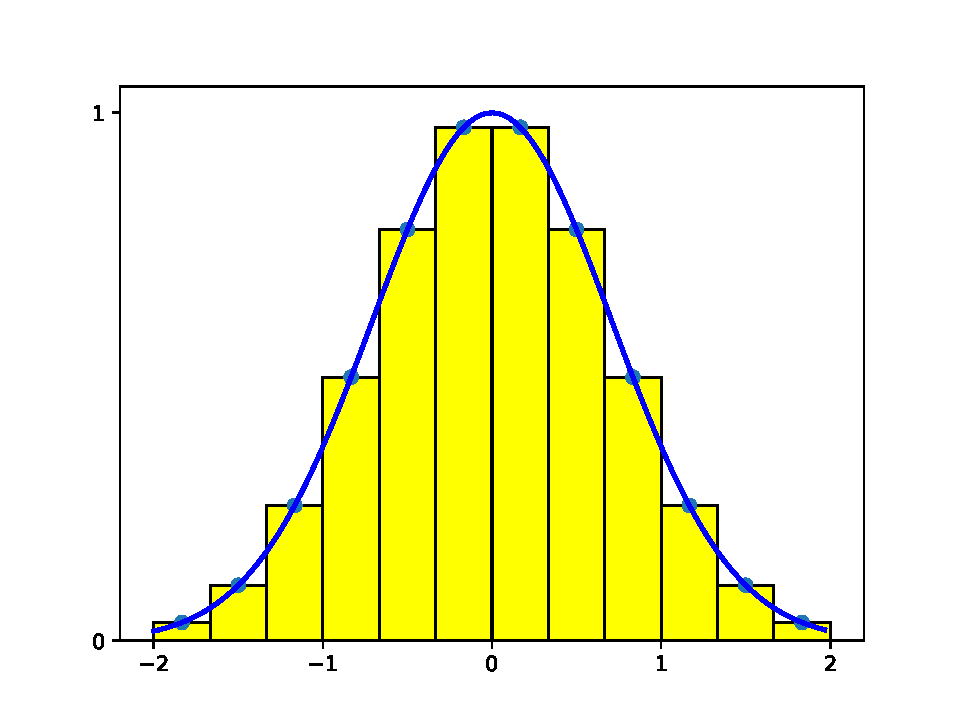
\includegraphics[width=10cm]{pics/riemann_sum.pdf}
\end{center} 
\end{bem} 

\begin{defn}[Orientierte Version des Riemann-Integrals] 
	Wir haben $\int_a^b f(x) \dd x$ für $a<b$ definiert. Nun setzen wir
	\begin{align*}
		\int_a^b f(x) \dd x = \begin{cases}
			0, &  \ \text{für} \ a =b, 
			\\ - \int_b^a f(x) \dd x  & \ \text{für} \ a > b.
		\end{cases} 
	\end{align*} 
\end{defn} 

\begin{bem}[Leinbiz'sche Intuition beim bestimmten Integral]
	$\dd x$ ist die unendlich kleine Änderung von $x$ innerhalb eines unendlich kleinen Intervalls. 
	$f(x) \dd x$ ist die unendlich kleine Änderung von $x$ mal der Wert von $f$ in einem unendlich kleinen Interval. Das Integral $\int_a^b f(x) \dd x$ ist eine unnendliche Summe all der unendlich kleinen Werte $f(x) \dd x$ für die unendlich kleinen Intervalle, die $[a,b]$ pflastern (bei $a<b$). 
\end{bem} 



\section{Grundeigenschaften des Riemann-Integrals} 

\begin{thm} 
	Eine Riemann-integrierbare Funktion $f$ auf $[a,c]$ ist auf jedem Unterintervall von $[a,c]$ ebenfalls Riemann-integrierbar und es gilt
	\[
	\int_a^c f(x) \dd x = \int_a^b f(x) \dd x+ \int_b^c f(x) \dd x
	\]
	für alle $b \in [a,c]$. 
\end{thm} 


\begin{thm} 
	Sind $f, g$ Riemann-integrierbar über $[a,b]$ und $\alpha, \beta \in \R$, dann sind auch $f \cdot g$ und $\alpha f + \beta g$ Riemann integrierbar, uns es gilt: 
	\[
			\int_a^b (\alpha f(x) + \beta g(x) ) \dd x = \alpha \int_a^b f(x) + \beta \int_a^b g(x) \dd x. 
	\]
\end{thm} 

\begin{thm} 
	Jede stetige Funktion auf $[a,b]$ ist Riemann-integrierbar. 
\end{thm} 

\begin{thm}
	Jede beschränkte Funktion auf $[a,b]$, die in nur in endlich vielen Punkten von $[a,b]$ nicht stetig ist, ist Riemann-integrierbar. 
\end{thm} 

\begin{bem}
	Ungleichungen können integriert werden...
\end{bem} 

\begin{thm}
	Sind $f$ und $g$ über $[a,b]$ Riemann-integrierbar, dann folgt aus $f(x) \le g(x)$ für alle $x \in [a,b]$ die Ungleichung 
	\[
		\int_a^b f(x) \dd x \le \int_a^b g(x) \dd x.
	\]
\end{thm} 

\begin{defn}
	Gilt für Funktionen $f, F: I \to \R$ auf einem Intervall $I$ die Relation $F' = f$ so nennt man $F$ \emph{Stammfunktion} von $f$. 
\end{defn} 

\begin{bem} 
	Sind $F_1, F_2$ Stammfunktion von $ f: I \to \R$, dann ist ihre Differenz $F_1 - F_2$ eine Konstante Funktion auf dem Intervall $I$. Das folgt aus dem Mittelwertsatz der Differentialrechnung. Die Tatsache, dass $I$ ein Intervall ist, ist wesentlich. 
\end{bem} 

\begin{defn} 
	Das \textbf{unbestimmte Integral} einer Funktion $ f: I \to \R$ auf einem Intervall $I$ ist die parametrische Familie aller Stammfunktionen von $f$. Bezeichnung: $\int f(x) \dd x$. 
\end{defn} 

\begin{bem}
	Das Integral $\int_a^b f(x) \dd x$ nennt man im Gegensatz zum unbestimmten Integral $\int f(x) \dd x$ das \textbf{bestimmte Integral}. 
\end{bem} 

\begin{bsp}
		Es gilt
		\[\int \cos x \dd x= \sin x + C\] 
		wegen 
		\[
			(\sin x + C)' = \cos x.
		\]
		Hier steht $C \in \R$ für eine Konstante. 
		
		Der Ausdruck $\sin x+ C$ steht hier eigentlich für die Menge $\setcond{ \sin x+ C}{C \in \R}$ aller Stammfunktion von $\cos  x$, es ist aber üblich in solchen Situation die Schreibweise $\sin x+ C$ zu benutzen. 
\end{bsp} 

\begin{bem}
	Die Formeltafeln für die Stammfunktionen sind im Wesentlichen die Formeltafeln für Ableitungen, die man ``rückwärts'' aufgeschrieben hat. Zum Beispiel: 
	
	\begin{align*}
		(\sin x)'  & = \cos x  & & \Longleftrightarrow & \int \cos x \dd x & = \sin x + C,
	\\	(\cos x)'  & = - \sin x  & & \Longleftrightarrow & \int \sin x \dd x & = - \cos x + C,		
	\\ (x^p)' & = p x^{p-1} & & \Longleftrightarrow & \int x^a \dd x & = \frac{x^{a+1}}{a+1} + C \qquad (\text{für} \ a \ne -1),
\\	& & & \quad\vdots 
	\end{align*} 
\end{bem} 

\begin{bem}
	Das unbestimmte und das bestimmte Integral hängen zusammen... 
\end{bem} 

\begin{thm}[Hauptsatz der Differential- und Integralrechnung]  
	Ist $F$ Stammfunktion von $f : [a,b] \to \R$, so gilt 
	\[
		\int_a^b f(x) \dd x = F(b) - F(a). 
	\]
\end{thm} 

\begin{bem} 
	Als Folgerung können wir die Ableitung von $\int_a^x f(t) \dd t$ nach $x$ bestimmen. Ist $F$ Stammfunktion von $f$, so gilt 
	\[
		\int_a^x f(t) \dd t = F(x) - F(a).
	\]
	Es folgt
	\[
		\left(\int_a^x f(t) \dd t \right)' = (F(x)-F(a))' = F'(x) = f(x). 
	\]
	Wir haben gezeigt, dass $\int_a^x f(t) \dd t$ als Funktion in $x$ Stammfunktion von $f(x)$ ist. 
\end{bem} 

\begin{bem} 
	Für $F(b) - F(a)$ benutzt man die folgenden Bezeichnungen:  $\bigl.F(x)\bigr|_{x=a}^b$  oder $\bigl.F(x)\bigr|_a^b$ oder  $\bigl[ F(x) \bigr]_a^b$ oder $\bigl.[ F(x) \bigr]_{x=a}^b$.
\end{bem} 

\begin{bem}[Leibniz'sche Intuition hinter dem Hauptsatz der Differential- und Integralrechnung] 
	Die Formel $\int_a^b F'(x) \dd x = F(b) - F(a)$ kann man intuitiv durch $F'(x) \dd x = \frac{\dd F}{\dd x} \dd x = \dd F$ erklären. Das $\dd F$ ist also eine Änderung von $F$ in einem unendlich kleinen Intervall der Länge $\dd x$. Diese Änderungen von $F$ summieren sich in $\int_a^b \dd F$ zur Änderung $F(b) - F(a)$ innerhalb von $[a,b]$. 
\end{bem} 

\begin{bem} 
	Im Folgenden werden Regeln diskutieren, die man beim Ausrechnen von Integralen benutzen kann. Man muss aber gewarnt werden, dass nicht jede elementare Funktion eine elementare Stammfunktion besitzt.  Eines der bekanntesten Beispiele ist die Funktion $e^{-x^2}$. Es gilt
	\[
		\int e^{-x^2} \dd x = F(x) + C,
	\]
	für die Stammfunktion $F$ (das  ist die Funktion mit $F'(x) = e^{-x^2}$) hat man aber keine elementare Formel. Das bedeutet unter anderem, dass man zur Berechnung des bestimmten Integrals 
	\[
		\int_a^b e^{-x^2} \dd x
	\]
	für gegebene $a$ und $b$ numerische Approximationen benutzen muss (Stichwort: Numerisches Integrieren). 
\end{bem} 

\begin{bsp}
	Wir berechnen das Volumen eines Kegels $K$ in $\R^3$ in Abhängigkeit von der Grundfläche und der Höhe. Sei $A$ der Flächeninhalt der Grundfläche des Kegels und $h$ die Höhe. 
	
	Wir platzieren den Kegel im Raum $\R^3$ so, dass die Spitze in $(0,0,0)$ ist und die Grundfläche in der Ebene $\{h\} \times \R^2$ liegt. Für $x \in [0,h]$ hat der Querschnitt des Kegels mit der Ebene $\{x\} \times \R^2$ die Fläche 
	\[
		f(x) := \left( \frac{x}{h} \right)^2 A,
	\]
	
	Wenn wir im Bereich $[0,h]$ eine Zerlegung $Z = \{x_0,\ldots,x_n\}$ mit $0=x_0 < \cdots < x_n \le n$ einführen, dann ist der ``Ausschnitt'' $\setcond{ (x,y,z) \in K}{ x_{i-1} \le x \le x_i}$ des Kegels $K$ ein Kegelstumpf, den man zwischen zwei Zylindern schachteln kann:  die beiden Zylinder haben Höhe $x_i - x_{i-1}$, der kleinere Zylinder hat die Fläche $f(x_{i-1})$ und der größere Zylinder hat die Fläche $f(x_i)$. Wir haben also das Volumen $V$ des Kegels durch 
	\[
	 \sum_{i=1}^n (x_i - x_{i-1}) f(x_{i-1}) = U_f(Z) \le V \le O_f(Z) \le \sum_{i=1}^n (x_i-x_{i-1}) f(x_i)
	\] approximiert. Da man $U_f(Z) \le V \le O_f(Z)$ hat und die Zerlegung $Z$ beliebig ist, sehen wir dass  $V = \int_0^h f(x) \dd x$ ist. 
	
	
 Wir erhalten also für das Volumen die Beschreibung
	\begin{align*}
		V & = \int_0^h \left( \frac{x}{h} \right)^2 A \dd x
		\\ & = \frac{A}{h^2} \int_0^h x^2 \dd x
		\\ & = \frac{A}{h^2} \biggl[ \frac{1}{3} x^3 \biggr]_{x=0}^h
		\\ & = \frac{A}{h^2} \cdot \frac{h^3}{3} 
		\\ & = \frac{1}{3} h A. 
	\end{align*}
\end{bsp} 


\section{Substitutionsregel} 

\begin{bem}[Substitution]
	
	Sei $F$ Stammfunktion von $f$ und sei $g$ differenzierbar. Die Kettenregel ergibt: 
	\[
		(F \circ g)' = (F' \circ g) \cdot g' = (f \circ g) \cdot g'. 
	\]
	Das heißt: $F \circ g$ ist eine Stammfunktion von $(f \circ g) \cdot g'$. Das kann man als die Gleichung 
	\[
		\int f ( g(x)) g'(x) \dd x = F(g(x)) + C
	\]
	für das unbestimmte Integral von $f (g(x)) g'(x)$ 
	hinschreiben. Durch das Anwenden des Hauptsatzes ergibt sich daraus die Substitutionsregel für bestimmte Integrale: 
	\[
		\int_a^b f(g(x)) g'(x) \dd x = \int_{g(a)}^{g(b)} f(y) \dd y. 
	\]
	Tatsächlich: Nach dem Hauptsatz kann man die linke Seite als $(F \circ g)(b) - (F \circ g)(a)$ umschreiben und die rechte Seite als $F(g(b)) - F(g(a))$. Das ist aber dasselbe. 
\end{bem} 

\begin{bem}[Leibniz'sche Sichtweise] 
	Erinnern wir uns an die Schreibweise von Leibniz: 
	\[
		q'(x) = \frac{\dd q(x)} {\dd x}. 
	\]
	Wenn wir nun diese Gleichung rein formal als $\dd q(x)  = q'(x) \dd x$ umschreiben, so werden wir motiviert, die folgende Bezeichnung einzuführen: 
	\[
		\int p(x) \dd q(x) := \int p(x) q'(x) \dd x 
	\]
	Hier noch die analoge Bezeichnung für bestimmte Integrale: 
	\[
		\int_a^b p(x) \dd q(x) := \int_a^b p(x) q'(x) \dd x
	\]
	
	Mit diesen Bezeichnungen kann nun die Substitutionsregel so beschrieben werden. 
	\begin{itemize}
		\item \emph{Für unbestimmte Integrale}. Zum Berechnen von \[
		\int f(g(x)) \dd g(x)
		\] reicht es aus, 
		\[ \int f(y) \dd y
		\] zu berechnen ($y$ ist neue Integrationsvariable) und dann \[ y=g(x) \] einzusetzen. Als Formel: 
		\[
			\int f(g(x)) \dd g(x) = \left. \left( \int f(y) \dd y \right) \right|_{y = g(x)}.
		\] 
		\item \emph{Bestimmte Integrale}. 
		\[
			\int_a^b f(g(x)) \dd g(x) = \int_{g(a)}^{g(b)} f(y) \dd y. 
		\] 
	\end{itemize} 
\end{bem} 

\begin{bsp}[Substitution für unbestimmte Integrale]
	\begin{align*}
		\int e^{-x^2} x \dd x & = -\frac{1}{2} \int e^{-x^2} \dd (- x^2)  & & | \text{ wegen} \ (x^2)' = 2 x
		\\ & = - \frac{1}{2} \int e^{y} \dd y & & | \text{ mit} \ y=-x^2.
		\\ & =  - \frac{1}{2} e^y + C & & | \ e^y \ \text{Stammfunktion von}  \ e^y
		\\ & =  - \frac{1}{2} e^{-x^2} + C 	 & & | \ y=-x^2 \ \text{einsetzen}.
	\end{align*} 
\end{bsp} 

\begin{bsp}[Substitution für bestimmte Integrale]
	\begin{align*}
		\int_0^{\pi/3} \tan(x) \dd x & = \int_{0}^{\pi/3} \frac{\sin x \dd x}{\cos x} & &|\text{ $\tan(x)$ ausschreiben}
		\\ & = - \int_0^{\pi/3} \frac{\dd \cos x}{\cos x}  & &|\text{ wegen} \ (\cos x)' =-\sin x 
		\\ & = - \int_{\cos 0}^{\cos \pi/3} \frac{\dd y}{y}  & &|\text{ mit}\  y=\cos x
		\\ & = - \int_1^{1/2} \frac{\dd y}{y} & &| \text{ Grenzen ausgerechnet}
		\\ & =  - \biggl[ \ln y \biggr]_1^{1/2} 
		\\ & = - (\ln 1/2 - \ln 1)
		\\ & = \ln 2.
	\end{align*}
\end{bsp} 




\section{Partielle Integration} 

\begin{bem}
	Partielle Integration ist die Umkehrung der Produktregel für das Differenzieren. 
	Die Produktregel besagt
	$( u(x) v(x))'= u'(x) v(x) + v'(x) u(x)$. Das bedeutet
	\[
		\int ( u'(x) v(x) + u(x) v'(x)) \dd x = u(x) v(x)+ C.
	\]
	Somit ergibt sich die Gleichung 
	\[
		\int u(x) v'(x) \dd x = u(x) v(x) - \int u'(x) v(x) \dd x
	\]
	 für zwei unbestimmte Integrale. Die Ableitung ``wandert'' von $v$ auf $u$, was in manchen Situationen zur einer Vereinfachung des Integrals führt.  
	 
	 Wir können die Gleichung auch in den folgenden Bezeichnungen formulieren: 
	 \[
	 	\int u(x) \dd v(x) = u(x) v(x) - \int v(x) \dd u(x) 
	 \]
\end{bem} 

\begin{bsp}[Partielle Integration für unbestimmte Integrale]
	\begin{align*}
		\int x^2 e^x \dd x & = \int  x^2 \dd e^x & & |\text{ wegen} \ (e^x)'= e^x
		\\ & = x^2 e^x  - \int e^x \dd x^2 & & |\text{ partiell integrieren}
		\\ & = x^2 e^x  - 2 \int x e^x \dd x & & |\text{ wegen} \ (x^2)' = 2x
		\\ & = x^2 e^x - 2 \int x \dd e^x & & |\text{ wegen} \ (e^x)' = e^x
		\\ & = x^2 e^x  - 2 x e^x + 2 \int e^x \dd x & &|\text{ partiell integrieren}
		\\ & = x^2 e^x  - 2 x e^x + 2 e^x + C & & |\text{ wegen} \ (e^x)'= e^x
		\\ & = (x^2 - 2 x+ 2) e^x + C.
	\end{align*}
\end{bsp} 

\begin{bsp}
	\begin{align*}
		\int \ln x \dd x & = x \ln x - \int x \dd \ln x & &| \text{\ partielle Integration}
		\\ & = x \ln x - \int x \frac{1}{x} \dd x & &| \text{\ wegen} (\ln x)' = \frac{1}{x}
		\\ & = x \ln x  - \int \dd x 
		\\ & = x \ln x - x + C
	\end{align*} 
\end{bsp} 

\begin{bem}
	Partielle Integration für bestimmte Integrale: 
	\[
		\int_a^b u(x) v'(x) \dd x = \biggl[ u(x) v(x) \biggr]_{x=a}^b - \int_a^b u'(x) v(x) \dd x. 
	\]
\end{bem} 

\section{Uneigentliche Integrale} 

\begin{bsp} 
	Das Integral 
	 $\int_0^1 x^{-1/2} \dd x$ existiert im Rahmen der oben angeführten Theorie der Riemann-Integrale nicht. Die Funktion $x^{-1/2}$ ist an der unteren Grenze $0$ nicht definiert. Auch wenn wir die Funktion auf die Stelle erweitern würden, wäre eine solche Erweiterung über $[0,1]$ nicht Riemann-integrierbar. Wir können das Integral as ein sogenanntes \textbf{uneigentliches Integral} folgendermaßen einführen: 
	 \[
	 	\int_0^1 x^{-1/2} \dd x = \lim_{h \to 0 + } \int_h^1 x^{-1/2} \dd x.
	 \]
	 Weil man 
	 \[
	 		\int_h^1 x^{-1/2} \dd x = \biggl[ 2 x^{1/2} \biggr]_{x=h}^1 = 2 - 2 \sqrt{h} 
	 \]
	 hat, erhalten wir 
	 \[
	 	\int_0^1 x^{-1/2} \dd x = \lim_{h \to 0+} ( 2  - 2\sqrt{h} ) = 2.
	 \] 
\end{bsp} 

\begin{bsp}
	Wir können das Integrieren über unbeschränkte Intervalle ebenfalls als uneigentliche Integrale einführen. Zum Beispiel:
	\[
		\int_0^\infty e^{-x} \dd x = \lim_{t \to \infty} \int_0^t e^{-x} \dd x. 
	\]
	Weil man 
	\[
		\int_0^t e^{-x} \dd x = \biggl[ - e^{-x} \biggr]_{x=0}^t = 1 - e^{-t}
	\]
	hat, erhalten wir 
	\[
		\int_0^\infty e^{-x} \dd x = \lim_{t \to \infty} (1 - e^{-t}) = 1. 
	\]
	Diese Berechnung wird in der Regel folgendermaßen aufgeschrieben: 
	\[
		\int_0^\infty e^{-x} \dd x = \biggl[ -e^{-x} \biggr]_{x=0}^\infty  = 1 - 0 = 1, 
	\]
	wobei man unter dem Einsetzen von $\infty$ einen Grenzwertübergang meint. 
\end{bsp} 

\begin{defn}[Verschiedene uneigentliche Integrale] 
	Seien $-\infty < a< b < \infty$. Wir definieren die uneigentlichen Integrale:
	\begin{align*}
		\int_a^\infty f(x) \dd x & := \lim_{t \to \infty} \int_a^t f(x) \dd x,
		\\ \int_{-\infty}^b f(x) \dd x & := \lim_{t \to -\infty} \int_t^b f(x) \dd x,
		\\ \int_{-\infty}^\infty f(x) \dd x & := \int_{-\infty}^0 f(x) \dd x + \int_0^\infty f(x) \dd x,
		\\ \int_a^b f(x) \dd x & := \lim_{h \to 0+} \int_{a+h}^b f(x) \dd x,  & & \text{bei} \ \lim_{h \to 0+} |f(a+h)| =\infty.
		\\ \int_a^b f(x) \dd x & := \lim_{h \to 0+} \int_a^{b-h} f(x) \dd x, & & \text{bei} \ \lim_{h \to 0+} |f(b-h)| = \infty. 
	\end{align*} 
\end{defn} 

\begin{bem}
	Da uneigentliche Integrale Grenzwerte sind, kann man für sie die Terminologie aus der Theorie der Grenzwert benutzen (Konvergenz, Divergenz, bestimmte Divergenz). 
\end{bem} 

\begin{bsp} 
	\begin{align*}
		\int_{-\infty}^\infty \frac{\dd x}{x^2 + 1} & = \biggl[ \arctan x \biggr]_{x=-\infty}^\infty 
		\\ & = \lim_{x \to \infty} \arctan x - \lim_{x \to -\infty} \arctan x 
		\\ & = \frac{\pi}{2} - \left( - \frac{\pi}{2} \right) 
		\\ & = \pi 
	\end{align*}
\end{bsp} 

\section{Exkurs in Lebesgue-Integrale}

\begin{bem}
	Uneigentliche Integrale sind eine ``schnelle Reparatur'' einiger Probleme, die man mit der Theorie der Riemann-Integrale hat. Man kann über unbeschränkten Bereichen nicht direkt nach Riemann integrieren, man kann viele (gute) unbeschränkte Funktionen nicht direkt nach Riemann integrieren. 
	
	Eine ``grundsätzliche Reparatur'' bietet die Theorie von \textbf{Lebesgue-Integralen}. Lebesgue-Integrierbarkeit ist eine viel weniger einschränkende Eigenschaft einer Funktion.  In der Theorie der Lebesgue-Integrale müssen die Integrale 
	\begin{align*}
		\int_0^1 x^{-1/2} \dd x & = 2, & &\text{und} & \int_0^\infty e^{-x}  \dd x& = 1
	\end{align*}
	nicht gesondert behandelt werden: die beiden Funktionen sind über die jeweiligen Bereichen Lebesgue-integrierbar. 
\end{bem} 

\begin{bem}
	Basics zu Lebesgue-Integralen:
	\begin{enuma} 
		\item In der Definition des Lebesgue-Integrals zerlegt man nicht den Defintionsbereich sondern den Wertebereich in Stückchen. 
		\item Definition des Lebesgue-Integrals für Funktion einer Variable basiert auf dem Lebesgue-Maß in $\R$, d.h., für mache Teilmengen von $\R$ kann ihre Länge (im Lebesgue-Sinne) messen. Hierbei ist die Länge von $[a,b]$ gleich  $b-a$. Die Länge von $[a,b] \cap \Q$ ist aber zum Beispiel $0$, weil $[a,b] \cap \Q$ aus abzählbar vielen einelementigen Mengen zusammengesetzt ist, deren Länge gleich $0$ ist. 
		\item Wenn die Gleichung $\int_a^b f(x) \dd x = I$ nach der Definition von Riemann gilt, nach gilt sie auch nach der Definition von Lebesgue. Das heißt, das Riemann-Integral ist eine Ereweiterung des Lebesgue-Integrals. 
	\end{enuma} 
\end{bem} 

\begin{bem}[Lebesgue-Integral und Wahrscheinlichkeitstheorie]
	Für die Wahrscheinlichkeitstheorie reicht die Theorie der Riemann-Integrale nicht aus. Lebesgue-Integrale sind mit Hinblick auf Anwendungen in Wahrscheinlichkeitstheorie sehr natürliche Objekte. 
\end{bem} 

\section{Abschätzung von Summen und Reihen durch Integrale}

\begin{bem}
	Summen, Reihe und Integrale sind alles Varianten von Summen. Obwohl Integral umsetzungstechnisch die kompliziertesten Varianten von Summen sind, sind sie oft einfacher zu Berechnen als Summen oder Reihen. Was man also machen kann: Summen und Reihen durch Integrale Abschätzen. 
\end{bem} 

\begin{bsp}[Partialsumme der harmonischen Reihe]
	Wir geben Abschätzungen für 
	\[
		s_n := \sum_{k=1}^n \frac{1}{k}
	\]
	
	Die Abschätzung von $s_n$ basiert auf dem Vergleich von $s_n$ mit den bestimmten Integralen der Funktion $\frac{1}{x}$. 
	
	
	Hier die graphische Illustration im Fall $n=5$. Wir haben fünf Balken der Höhen $1, 1/2, 1/3, 1/4, 1/5$ und stellen die Balken der Höhen $1/2,1/3,1/4$ und $1/5$ unter den Graphen der Funktion $1/x$ auf dem Bereich $[1,5]$. Das ermöglicht die Abschätzung von $1/2+1/3 + 1/4 + 1/5 \le \int_1^5 \frac{1}{x} \dd x$. 
	\begin{center} 
		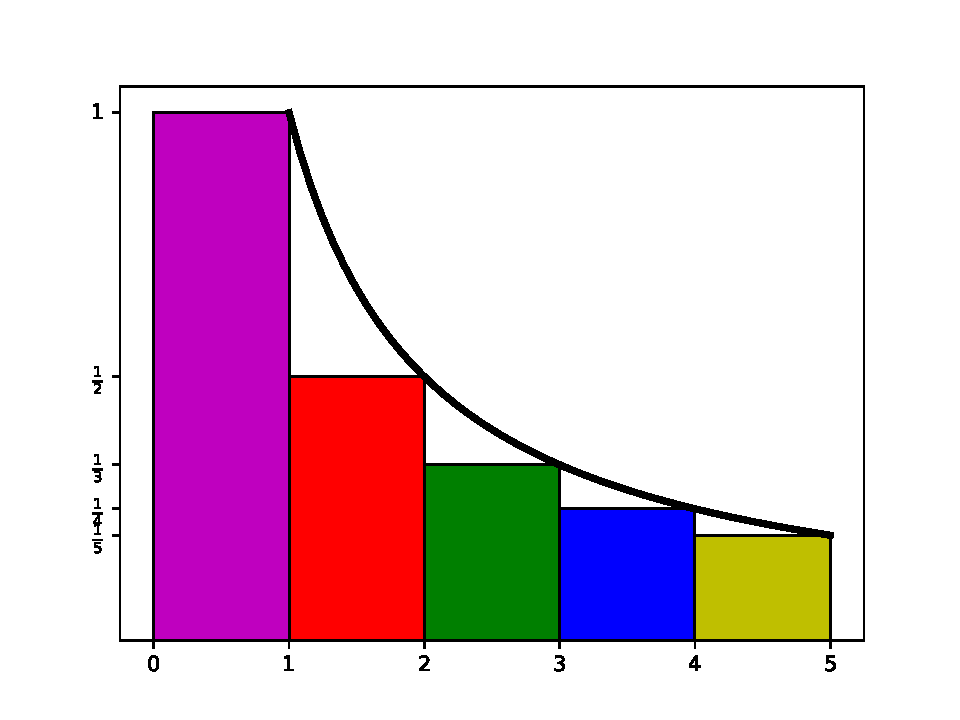
\includegraphics[width=0.7\textwidth]{pics/harmonic_number_upper.pdf}
	\end{center} 

	Wir können auch alle fünf Balken auf dem Bereich $[1,6]$ abstellen. Dann geht der Graph Funktion $\frac{1}{x}$ durch die Balken durch und ``sägt'' die oberen Teile der Balken ab: 
	\begin{center} 
	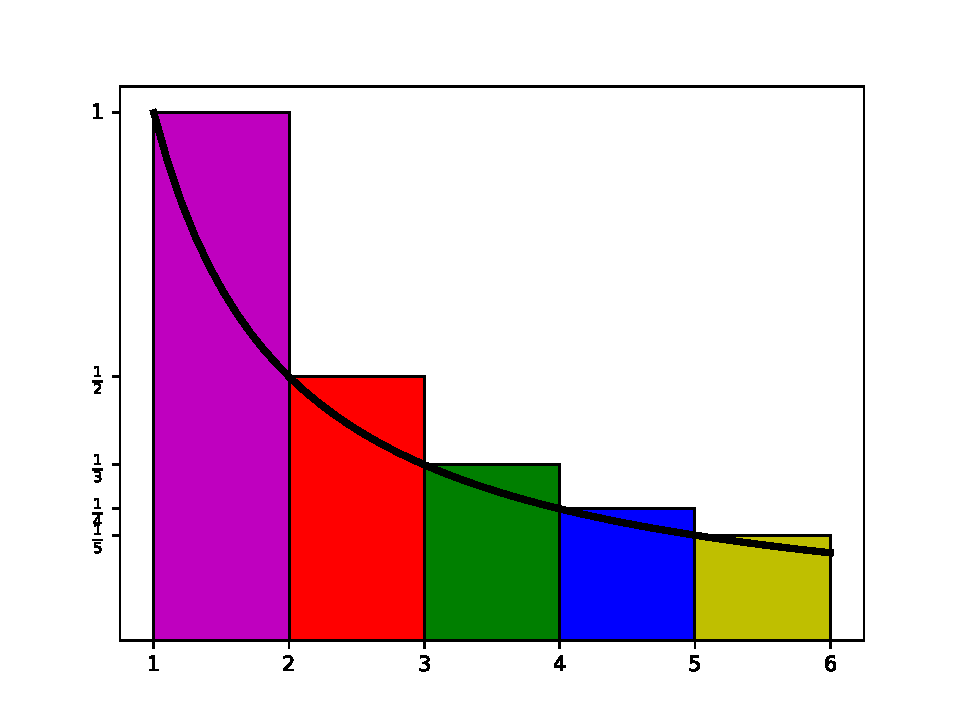
\includegraphics[width=0.7\textwidth]{pics/harmonic_number_lower.pdf}
\end{center} 
	Das ergibt die Abschätzung $1 + 1/2 + 1/3 + 1/4 + 1/5 \ge \int_1^6 \frac{1}{x} \dd x$.

	
	
	Obere Schranke: 
	\begin{align*}
		s_n & = \sum_{k=1}^n \frac{1}{k} 
		\\ & = 1 + \sum_{k=2}^n \frac{1}{k}
		\\ & = 1 + \sum_{k=2}^n \int_{k-1}^k \frac{1}{k} \dd x & & |\text{ wegen} \ \int_{k-1}^k \dd x = 1
		\\ & \le 1 + \sum_{k=2}^n \int_{k-1}^k \frac{1}{x} \dd x & & |\text{ wegen} \ x \le k \ \text{für} \ x \in [k-1,k]
		\\ & = 1 + \int_1^n \frac{1}{x} \dd x & & |\text{ Integrale zusammenfassen}
		\\ & = 1 + \biggl[ \ln x \biggr]_{x=1}^n
		\\ & = 1 + \ln n.
	\end{align*}
	Das ergibt
	\[
		s_n \le 1 + \ln n.
	\]
	
	
	Untere Schranke: 
	\begin{align*}
		s_n & = \sum_{k=1}^n \int_k^{k+1} \frac{1}{k} \dd x  & & |\text{ wegen} \ \int_k^{k+1} \dd x = 1.
		\\ & \ge \sum_{k=1}^n \int_k^{k+1} \frac{1}{x} \dd x & & |\text{ wegen} \ x \ge k \  \text{für} \ x \in [k,k+1].
		\\ & = \int_1^{n+1} \frac{1}{x} \dd x & & |\text{ alle $n$ Integrale zusammengefügt}
		\\  & = \biggl[ \ln x \biggr]_{x=1}^{n+1} 
		\\ & = \ln (n+1). 
	\end{align*}
	Das ergibt: 
	\[
		s_n \ge \ln (n+1). 
	\]
	
	Hier $s_n$ im Vergleich zu $\ln x$ und $1 + \ln x$: 
	
	\begin{center}
		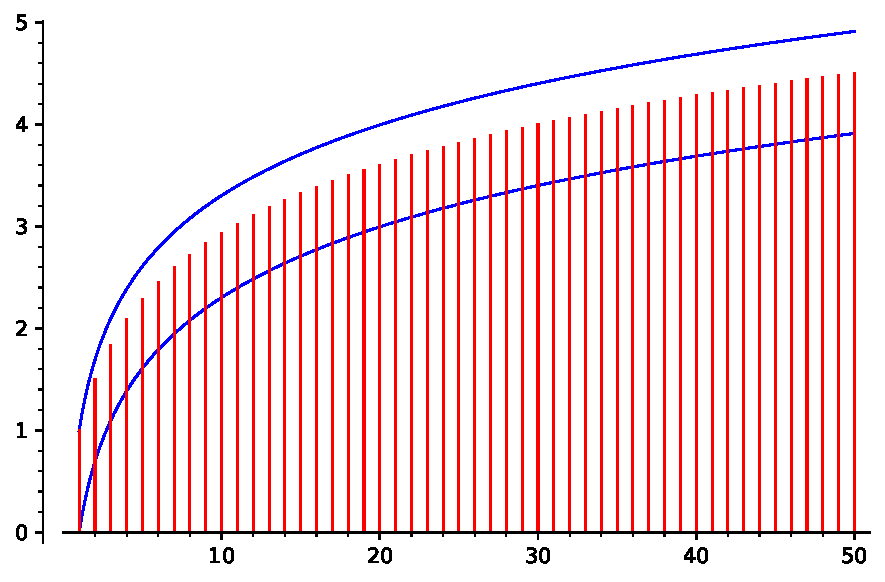
\includegraphics[width=0.8\textwidth]{pics/partial_sums_harmonic_series.pdf} 
	\end{center} 
\end{bsp} 

\begin{bsp}
	Wir wissen, dass die harmonische Reihe $\sum_{k=1}^\infty \frac{1}{k}$ divergent ist (das vorige Beispiel war ein weiterer Nachweis). Die harmonische Reihe ist Spezialfall $s=1$ der Reihe $\sum_{k=1}^\infty \frac{1}{k^s}$.

	Wir zeigen nun, dass $\sum_{k=1}^\infty \frac{1}{k^s}$ für $s>1$ konvergent ist. 
	\begin{align*}
		\sum_{k=2}^\infty \frac{1}{k^s} & = \sum_{k=2}^\infty \int_{k-1}^k \frac{1}{k^s} \dd x
			\\ & \le \sum_{k=2}^\infty \int_{k-1}^k \frac{1}{x^s} \dd x
			\\ & = \int_1^\infty \frac{1}{x^s} \dd x
			\\ & = \biggl[ \frac{1}{1-s} x^{1-s} \biggr]_{x=1}^\infty 
			\\ & = \frac{1}{s-1}
	\end{align*} 
	Das ergibt die Abschätzung
	\[
		\sum_{k=1}^\infty \frac{1}{k^s} = 1 + \sum_{k=2}^\infty \frac{1}{k^s} \le 1 + \frac{1}{s-1} = \frac{s}{s-1}
	\]
\end{bsp} 

\begin{aufg}
	Geben Sie eine untere Abschätzung an $\sum_{k=2}^\infty \frac{1}{k^s}$ für $s > 1$ durch eine Funktion in $s$. 
\end{aufg} 

\begin{aufg} 
	Nehmen wir an, Sie sind mit der Qualität der Abschätzung 
	\[
		\sum_{k=1}^\infty \frac{1}{k^s} \le \frac{s}{s-1}
	\]
	für $s > 1$ nicht ganz zufrieden. Sie erhalten zum Beispiel, für $s=\frac{11}{10}$. 
	\[
		\sum_{k=1}^\infty \frac{1}{k^{11/10}} \le 11
	\]
	und würden gerne die $11$ durch eine bessere Schranke ersetzen. Wie würden Sie vorgehen? 
\end{aufg} 

\begin{bem}
	Formulieren wir die vorigen Abschätzungen als ein allgemeines Prinzip. Sei $f : [0,+\infty) \to [0,+\infty)$ monoton fallend und sei $\int_0^\infty f(x) \dd x < +\infty$. Dann gilt
	\begin{align*}
		\int_1^\infty f(x) \dd x \le \sum_{k=1}^\infty f(k) & \le \int_0^\infty f(x) \dd x.
	\end{align*}
	Man kann also die Summe $\sum_{k=1}^\infty f(k)$, die man evtl. nicht exakt berechnen kann, durch die Berechnung der beiden Integrale von $f(x)$ (wenn man etwa die Stammfunktion von $f(x)$ exakt bestimmen kann) abschätzen. 
\end{bem} 

\begin{aufg}
	Vergewissern Sie sich, dass die Abschätzungen aus der vorigen Bemerkung tatsächlich stimmen. 
\end{aufg} 

\section{Integrale rationaler Funktionen}

\begin{defn}
	\textbf{Rationale Funktion} ist Quotient von Polynomen. 
\end{defn} 

\begin{bsp}
	Wir lesen die Formeltafeln für Ableitungen und bestimmen dadurch die Stammfunktion von $\frac{1}{x}$:
	\begin{align}
	\label{def:stamm:1/x}
	\int \frac{\dd x}{x} = \ln |x| + C. 
	\end{align}
	
	\begin{itemize}
		\item Mann beachte, dass weder $\frac{1}{x}$ noch $\ln |x|$ in $0$ definiert ist. 
		\item Formel \eqref{def:stamm:1/x} bedeutet: fixiert man ein Intervall $I$, das $0$ nicht enthält, so ist 
		\[
		\setcond{\ln |x| + C}{C \in \R}
		\] die Menge aller Funktionen auf $I$, deren Ableitung gleich $\frac{1}{x}$ ist. 
		\item Formel \eqref{def:stamm:1/x} kann für die Berechnung bestimmter Integrale benutzt werden, man sollte aber die oben angeführten Kommentare beachten:
		\begin{align*}
		\int_1^e \frac{\dd x}{x} & = \ln |e| - \ln |1| = 1  & & |\text{ alles okay}
		\\ \int_{-4}^{-2} \frac{\dd x}{x} & = \ln |-2| - \ln |-4| = - \ln 2  & & |\text{ alles okay}
		\\ \int_{-3}^1 \frac{\dd x}{x} &  \tikz[baseline=-4]{\node at (0,0) {\(= \ln |1| - \ln |-3| \)}; \draw[red, thick] (-1.5,-0.5) -- (1.5,0.5); \draw[red,thick] (-1.5,0.5) -- (1.5,-0.5); } & & |\text{ nicht okay wegen $0 \in [-3,1]$} 
		\end{align*}
	\end{itemize} 
\end{bsp} 

\begin{bsp}
	Für $a \in \R \setminus \{0\}$ und $b \in \R$ kriegt man 
	\[
	\int \frac{\dd x}{a x+ b} = \frac{1}{a} \ln |a x + b| + C.
	\]
	durch die Substitution $y = a x + b$. 
\end{bsp} 

\begin{bsp} 
	Für $p \ne -1$ kriegt man 
	\[
	\int x^{p} \dd x = \frac{x^{p+1}}{p+1} + C,
	\]
	indem man die Formeltafeln für Ableitungen rückwärts liest. Zum Beispiel: $(x^{-3})'= -3 x^{-4}$ heißt, dass $-\frac{1}{3} x^{-3}$ Stammfunktion von $x^{-4}$ ist. Das schreibt man als 
	\[
	\int x^{-4}  \dd x = -\frac{1}{3} x^{-3} + C.
	\] 
\end{bsp} 

\begin{bsp} 
	Wir berechnen 
	\[
	\int \frac{x+1 }{x^2 + x -6 } \dd x.
	\]
	Mit der $pq$-Formel kann $x^2+ x -6$ als 
	\[
	x^2 + x - 6 = (x-2) (x+3)
	\] faktorisiert werden. Das zeigt
	\[
	\frac{x+1 }{x^2 + x -6 } =  \frac{x+1}{(x-2)(x+3)}.
	\]
	Nun kann man den Integranden als die Linearkombination
	\[
	\frac{x+1}{(x-2) (x+3)} = \frac{ A }{x-3} + \frac{B}{x-2}
	\]
	für gewisse $A, B \in \R$ darstellen. Wie bestimmt man $A$ und $B$? Erstmal die Gleichung mit $(x-2) (x+3)$ multiplizieren, sodass man auf die Gleichung 
	\begin{align}
	\label{eq:xAB}
	x + 1 = A \cdot (x-2) + B \cdot (x-3)
	\end{align}
	kommt. Nun kann man $A$ und $B$ aus der Gleichung \eqref{eq:xAB} durch den Koeffizientenvergleich bestimmen. Dafür müssen wir dann lineares Gleichungssystem mit zwei Gleichungen und den Unbekannten $A$ und $B$ lösen. 
	
	Noch einfacher geht es, wenn wir die Gleichung \eqref{eq:xAB} an $x =2$ und $x=3$ auswerten. Dann erhalten wir 
	\begin{align*}
	2 + 1 & = A \cdot (2-2) + B \cdot (2-3) = -B ,  & &| \text{ für} \ x =2
	\\ 3 + 1 & = A \cdot (3-2) + B \cdot (3-3) = A. &  &| \text{ für} \ x =3
	\end{align*}
	Wir haben nun die Darstellung 
	\[
	\frac{x+1}{(x-2) (x+3)} = \frac{4}{x-3} - \frac{3}{x-2}
	\]
	ermittelt. Unser ursprüngliches Integral wird also eine linear Kombination von zwei einfacheren Integralen dargestellt, die wir bereits kennen: 
	\begin{align}
	\nonumber \int \frac{x+1 }{x^2 + x -6 } \dd x & = 4 \int \frac{\dd x}{x-3} - 3 \int \frac{\dd x}{x-2} 
	\\ & = 4 \ln |x-3| - 3 |x -2| + C. \label{ln:3:2:C} 
	\end{align}
	Die Formel \eqref{ln:3:2:C} kann auch zur Berechnung bestimmter Integrale benutzt werden, solange weder $3$ noch $2$ im Integrationsbereich enthalten sind: 
	\begin{align*}
	\int_a^b \frac{x+1 }{x^2 + x -6 } \dd x & = \biggl[ 4 \ln |x-3| - 3 |x -2| \biggr]_{x=a}^b
	\end{align*}
	unter der Voraussetzung $[a,b] \cap \{2,3\} = \emptyset$. 
\end{bsp} 

\begin{bsp}
	Wir berechnen
	\[
	\int \frac{x^3 + 2 x^2 - 1}{x^2 + x -6} \dd x.
	\]
	Hier hat das Zähler-Polynom einen größeren Grad als das Nenner-Polynom. Wir dividieren Polynome mit Rest: 
	\begin{center}
		\polylongdiv{x^3+ 2 * x^2 -1}{x^2 + x - 6}
	\end{center}
	Das Originalintegral wird durch zwei einfachere Integrale ersetzt. 
	\[
	\int \frac{x^3 + 2 x^2 - 1}{x^2 + x -6} \dd x = \int (x+1) \dd x + 5 \int \frac{x+1}{x^2 + x-6} \dd x. 
	\]
	Die Stammfunktion von $x+1$ ist $\frac{1}{2} (x+1)^2$. Die Stammfunktion von 
	\( (x+1) / (x^2 + x - 6) \) haben wir im vorigen Beispiel ausgerechnet. 
\end{bsp} 

\begin{bsp} 
	\[
	\int \frac{\dd x}{x^2+ 1} = \arctan x + C,
	\]
	denn, wie wir wissen, ist $(\arctan x)' = \frac{1}{1+x^2}$. 
\end{bsp} 

\begin{bsp} 
	\begin{align*}
	\int \frac{\dd x}{x^2 + 4} & = \frac{1}{4} \int \frac{\dd x}{ (x/2)^2 + 1}  & & |\text{ wir brauchen $(\cdots )^2 + 1$ im Nenner}
	\\ & = \frac{1}{2} \int \frac{\dd (x/2) }{ (x/2)^2 + 1} & & | \ y=x/2 
	\\ & = \frac{1}{2} \int \frac{\dd y}{y^2 + 1} 
	\\ & =  \frac{1}{2} \arctan y + C
	\\ & = \frac{1}{2} \arctan (x/2) + C. 
	\end{align*}
	
	Natürlich kann man auf dieser Berechnung basierend auch eine allgemeine Formel erstellen: 
	\begin{align*}
	\int \frac{\dd x}{x^2 + a} & = \frac{1}{\sqrt{a}} \arctan \frac{x}{\sqrt{a}} + C & & \text{für} \ a > 0.
	\end{align*}
\end{bsp} 

\begin{bsp} 
	Wir berechnen
	\begin{align*}
	\int \frac{\dd x}{x^2 - 6 x + 18}
	\end{align*} 
	Die $pq$-Formel sagt uns, dass $x^2 - 6 x + 18$ keine reellen Nullstellen hat. Über reellen Zahlen können wir also $x^2 - 6 x + 18$ nicht in lineare Faktoren zerlegen. Wir machen die sogenannte quadratische Ergänzung. Dafür müssen wir die $18$ so in eine Summe zerlegen, dass wir mit einem Summanden zusammen mi $x^2-6 x$ die binomische Formel einsetzen können:
	\begin{align*}
	x^2 - 6 x + 18 & = x^2 - 6 x + 9 + 9 
	\\ & = (x-3)^2 + 9  & &| \text{ binomische Formel}
	\end{align*}
	Diese Darstellung des Nennerpolynoms, hilft uns das Integral zu berechnen: 
	\begin{align*}
	\int \frac{\dd x}{x^2 - 6 x + 18}	 & = \int \frac{\dd x}{(x-3)^2 + 9} 
	\\ & = \int \frac{ \dd (x-3) }{ (x-3)^2 + 9} 
	\\ & = \int \frac{ \dd y }{y^2  + 9} & &| \text{ mit} \ y=x-3
	\\ & = \frac{1}{3} \arctan \frac{y}{3} + C & &| \text{ nach dem vorigen Beispiel}
	\\ & = \frac{1}{3} \arctan \frac{x-3}{3} + C.
	\end{align*} 	
\end{bsp} 

\begin{bsp} 
	Es gilt
	\begin{align*}
	\int \frac{ (x+1) \dd x}{x^2 + 1} & = \int \frac{x \dd x}{x^2+ 1} + \int \frac{ \dd x}{x^2 + 1} 
	\end{align*}
	mit 
	\[
	\int  \frac{x \dd x}{x^2 + 1}  = \frac{1}{2} \int \frac{ \dd (x^2 + 1)}{x^2 + 1} = \frac{1}{2} \ln (x^2 + 1) + C.
	\]
	und 
	\[
	\int \frac{\dd x}{x^2 + 1} = \arctan x + C.
	\]
\end{bsp} 

\section{Integrale mit trigonometrischen Funktionen} 

\begin{bsp} 
	Zur Berechnung von 
	\[
		\int \cos^2 x \dd x .
	\]
	 können wir $\cos^2 x$ umformen. Durch 
	\begin{align*}
		\cos 2 x & = \cos^2 x - \sin^2 x  & &|\text{ Kosinus des doppelten Winkels} 
	\\	 & = \cos^2 x - (1- \cos^2 x) = 2 \cos^2 x -1 & &|\text{ Trigonometrischer Pythagoras} 
	\end{align*}
	erhalten wir eine Darstellung von $\cos^2 x$ mit Hilfe von $\cos 2 x$. Diese Darstellung benutzten wir nun: 
	\[
		\int \cos^2 x \dd x = \frac{1}{2} \int (1 + \cos 2 x) \dd x = \frac{1}{2} x + \frac{1}{4} \sin 2x + C.
	\]
	
	Hier noch eine Nebenbemerkung, die wir später bei Fourier-Reihen gebrauchen werden: es folgt 
	\begin{align*}
		\int_a^b \cos^2 x \dd x = \pi  & & \text{im Fall} \ b-a = 2 \pi. 
	\end{align*}
\end{bsp} 

\begin{aufg} 
	Berechnen Sie 
	\[
		\int \sin^2 x \dd x. 
	\]
\end{aufg} 

\begin{bsp}
	Wir berechnen 
	\[
		\int \cos^3 x \dd x.
	\]
	Wegen $\cos x \dd x = \dd (\sin x)$ und $\cos^2 x = 1 - \sin^2 x$ haben wir 
	\begin{align*}
			\int \cos^3 x \dd x & = \int (1- \sin^2 x) \dd \sin x 
			\\ & = \int (1 -y^2) \dd y & & |\text{ mit} \ y = \sin x
			\\ & = y - \frac{1}{3} y^3 + C
			\\ & = \sin x - \frac{1}{3} \sin^3 x + C.
	\end{align*}
\end{bsp} 

%\begin{bsp}
%	Wir berechnen 
%	\[
%		\int \frac{\dd x}{1 + \cos x} 
%	\]
%	Es ist bekannt, dass man $\cos x$ mit $\tan \frac{x}{2}$ darstellen kann. 
%	\begin{align*}
%		\cos x & = \cos^2 \frac{x}{2} - \sin^2 \frac{x}{2} & & |\text{ Nach der Formel für den Kosinus des doppelten Winkels}
%		\\ & = 2 \cos^2 \frac{x}{2}  - 1. 
%	\end{align*}
%	Anderseits hat man 
%	\[
%		\tan^2 \frac{x}{2}  = \frac{\sin^2 \frac{x}{2} }{\cos^2 \frac{x}{2} } = \frac{1- \cos^2 \frac{x}{2}}{\cos^2 \frac{x}{2}} = \frac{1}{\cos^2 \frac{x}{2}} - 1. 
%	\]
%	Wir haben also eine Gleichung, die $\cos x$ mit $\cos^2 \frac{x}{2}$ verlinkt und eine Gleichung, die $\tan^2 \frac{x}{2}$ mit $\cos^2 \frac{x}{2}$ verlinkt. Dadurch ist $\cos x$ mit $\tan^2 \frac{x}{2}$ verlinkt: 
%	\[
%		1 + \cos x = \frac{2}{1+\tan^2 \frac{x}{2}}.
%	\]
%	Unser Integral kann also als 
%	\[
%		\int \frac{\dd x}{1 + \cos x} = 2 \int \frac{\dd x}{1 + \tan^2 \frac{x}{2}}
%	\]
%	umgeschrieben werden. 
%	Es kann der Eindruck entstehen, dass unser Integral nach dieser Umformung nicht einfacher geworden ist, sondern eher komplizierter. Der Grund für die Umformung war, dass die Ableitung vom Arkustangens erstaunlich einfach ist. Sie ist nicht trigonometrisch sonder eine rationale Funktion! Wir führen die Integrationsvariable  $y = \tan \frac{x}{2}$ ein, was man auch als $x = 2 \arctan y$ hinschreiben kann. 
%	Das ergibt 
%	\[
%		\dd x =\dd (2 \arctan y) = \frac{2 \dd y}{1 + y^2}.
%	\]
%	So erhalten wir 
%	\begin{align*}
%		2 \int \frac{\dd x}{1 + \tan^2 \frac{x}{2} } & = 4 \int \frac{ \dd y}{(1+y^2)^2} 
%	\end{align*}
%\end{bsp} 

\chapter{Fourier-Reihen}

\section{Definition einer Fourier-Reihe}

\begin{defn}
	Sei $\omega> 0$. Eine \textbf{Fourier-Reihe}
	 ist Funktionsreihe der Form 
	\[
		\frac{a_0}{2} + \sum_{k=1}^\infty ( a_k \cos k \omega x + b_k \sin k \omega x). 
	\]
	Partialsummen 
	\[
		\frac{a_0}{2} + \sum_{k=1}^n (a_k \cos k \omega x + b_k \sin k \omega x)
	\]
	von Fourier-Reihen nennt man \textbf{trigonometrische Polynome}. 
\end{defn}

\begin{bem}
		Wir werden sehen, dass man mit einem geeigneten Definitions- und Wertebereich die Abbildung 
		\[
				f  \xmapsto{\quad\FR\quad}  (a_0,a_1,b_1,a_2,b_2,a_3, b_3, a_4, b_4\ldots )
		\]
		mit
		\[
				f(x) = \frac{a_0}{2} + \sum_{k=1}^\infty (a_k \cos k \omega x + b_k \sin k \omega x)
		\]
		definieren kann, die einer Funktion $f$ die Folge der Koeffizienten der Fourier-Reihe von $f$ zuordnet. Diese Abbildung ist \underline{linear} ist, d.h., es gilt 
		\[
				\FR(\alpha f + \beta g) = \alpha \FR(f) + \beta \FR(g)
		\]
		für Funktionen $f,g$ und $\alpha,\beta \in \R$. 
\end{bem} 

\begin{defn}
	Sei $T>0$. 
	Funktion $f : \R \to \R$ heißt \textbf{$T$-periodisch} wenn $f(x+T)= f(x)$ für alle $x \in \R$ erfüllt ist. Den Wert $T$ nennt man \textbf{Periode} von $f$. 
\end{defn}

\begin{bem}
	Glieder der Fourierreihe entstehen aus $T$-periodischen Funktionen $\cos k \omega x$ und $\sin k \omega  x$  mit $T = \frac{2 \pi}{\omega}$.  Die $T$-Periodizität von $f$ ist somit notwendig für die Zerlegbarkeit von $f$ in die Fourier-Reihe. 
\end{bem} 


\begin{bem}
	Warum man in der Fourier-Reihe die additive Konstante lieber als $\frac{a_0}{2}$ und nicht als $a_0$ darstellt, wird im Folgenden geklärt. Mit der Darstellung $\frac{a_0}{2}$ werden die Formeln für die Koeffizienten $a_k$ mit $k \in \N_0$ einheitlicher. 
\end{bem} 


\begin{bem}
	Die Konstante $\omega$ ist lediglich ein Skalierungsfaktor für $x$. Daher reicht es aus, den Fall $\omega =1$ zu betrachten, da man in der Fourier-Reihe $\omega x$ durch $x$ austauschen kann, um zum Fall $\omega =1$ kommen. Mit anderen Worten: um eine $T$-periodische Funktion $f(x)$ in eine Fourier-Reihe bzgl. $\omega = \frac{2\pi}{T}$ zu zerlegen, kann man die $2\pi$-periodische Funktion $f ( \frac{T}{2 \pi} x)$ bzgl. $\omega=1$ in die Fourier-Reihe zerlegen. 
\end{bem}

\begin{bem} 
	Eine $T$-periodische Funktion ist durch die Angabe auf einem Intervall $[a,b]$ der Länge $T$ eindeutig bestimmt. 
	
	Umgekehrt: eine Funktion $f : [a,b] \to \R$ auf einem Intervall der Länge $T$ und mit $f(a)=f(b)$, kann $T$-periodisch auf die gesamte reelle Achse eindeutig erweitert werden. 
\end{bem} 

\begin{bem}
	Ist $[a,b]$ Intervall der Länge $T>0$ und $f : \R \to \R$ eine $T$-periodische Funktion, die über $[0,T]$ integrierbar ist, so gilt 
	\[
		\int_a^b f(x) \dd x = \int_0^T f(x) \dd x,
	\]
	Das bedeutet: das Integral über jedes Intervall der Länge $T$ ist gleich. 
\end{bem} 

\section{Fourierreihen, Signalverarbeitung und weitere Anwendungen} 

\begin{bem}
	Fourier-Reihen wie auch ihre Analoga (Diskrete Fourier-Transformation und die Fourier-Transformation) haben sehr viele Anwendungen, die mit der Signalverarbeitung zusammenhängen, oder die Theorie von Schwingungen und Wellen im Hintergrund haben. 
	\begin{itemize}
			\item Signalverarbeitung allgemein
			\item Physik, unter anderem Astronomie und Optik
			\item Tomographie (insb. MRT und Ultraschaltomographie)
			\item Geologie
			\item Lösung von Differentialgleichungen 
	\end{itemize} 
\end{bem} 

\begin{bem}
	In der Signalverarbeitung ist $x$ der Zeitpunkt (wird deswegen auch oft als $t$ bezeichnet). Der Term	
	\[
	h_k(x):= a_k \cos k \omega x + b_k \sin k \omega x
	\] bestimmt die Phase und die Amplitude der $k$-ten Frequenz. Der Vektor $(a_k,b_k)$ kann in Polarkoordinaten als 
	\begin{align*}
		a_k & = A_k \cos \phi_k
		\\ b_k & = A_k \sin \phi_k
	\end{align*}
	mit $A_k \ge 0$ beschrieben werden. Dann gilt 
	\[
	h_k(x) := A_k \cos( k \omega x  - \phi_k). 
	\]
	Der Term $h_k(x)$ ist der Beitrag der $k$-ten Frequenz, $A_k$ ist die Amplitude und $\phi_k$ die Phase der $k$-ten Frequenz. 
\end{bem} 

\begin{bem} 
	Hier noch Kommentare zur Terminologie und Einheiten: 
	\begin{itemize}
		\item $x$ ist Zeit. Wir nehmen an, $x$ ist in Sekunden gegeben.
		\item $A_k$ ist die Amplitude. Die Einheiten von $A_k$ hängen von der Natur des Signals ab (elektrisch, mechanisch, akustisch usw.). 
		\item $k \omega$ ist die Kreisfrequenz von $h_k(x)$. Wenn man $k \omega x$ als einen Winkel, und somit als einen Punkt auf dem Einheitskreis interpretiert, dann ist $k \omega x$ die Geschwindigkeit dieses Punktes in Radianten pro Sekunde). Radianten sind dimensionslos, also ist die Einheit der Kreisfrequenz $\frac{1}{\text{Sekunde}} = \text{Hz}$.   
		\item $\frac{2 \pi}{k \omega}$ ist die Periode von $h_k(x)$ in Sekunden. In so viel Zeit  mach $k \omega x$ die volle Runde auf dem Einheitskreis. 
		\item $\frac{k \omega}{2 \pi} = (\frac{2 \pi}{k \omega})^{-1}$ ist die Anzahl der Runden pro Sekunde, also die Frequenz. Die Einheit dazu ist $\frac{1}{\text{Sekunde}} = \text{Hz}$.   
	\end{itemize}
\end{bem}  


\begin{bem}
	Bei der Darstellung in der ``Exponentialbasis'' ergibt sich die $k$-te Amplitude und Phase aus den Koeffizienten $c_k$ und $c_{-k}$. 
\end{bem} 

\section{Vektorräume,  Euklidische Räume und Hilberträume} 

\begin{defn} 
Ein (abstrakter) \textbf{Vektorraum} $V$ über einem Körper $\mathbb{K}$ ist eine Menge, die mit einem Skalarprodukt und einer Vektoraddition ausgestattet ist, für welche die folgenden Bedingungen erfüllt sind:
\begin{align*}
		a+ b & = b+ a
		\\ (a+b)+c & = a+(b+c) 
		\\ a+ \textbf{0} & = a
		\\ a + (-a) & = \textbf{0}
		\\ (\alpha + \beta) a & = \alpha a + \beta b
		\\ \alpha (a+b) & = \alpha a + \alpha b
		\\ \alpha (\beta a) & = (\alpha \beta) a
		\\ 1 \cdot a & = a. 
\end{align*} 
Hierbei sind $a,b,c \in V$ und $\alpha,\beta \in \mathbb{K}$. 
\end{defn} 

\begin{bem} 
	Man ist gewohnt, die konkreten Vektorräume wie $\R^3$ zu betrachten und in diesen Räumen zu rechnen: ,etwa
	\begin{align*}
			\begin{pmatrix}
				2 \\ 3 \\ 1 
			\end{pmatrix} 
			+ \begin{pmatrix} -1 \\ 0 \\ 4\end{pmatrix} 
			= \begin{pmatrix} 1 \\ 3 \\ 4 \end{pmatrix} 
	\end{align*} 
	 Die Definition eines abstrakten Vektorraums ist aber viel allgemeiner, sodass man nicht nur die Tupeln von reellen Zahlen als Vektoren auffassen kann. Um eine Menge $V$ als einen Vektorraum aufzufassen, braucht man für diese Menge $V$ eine sinnvolle Addition und eine sinnvolle Skalarmultiplikation. Sinnvoll heißt dabei, dass die definierenden Bedingungen des Vektorraums erfüllt sind. 
\end{bem} 

\begin{bsp}
	Die Funktionen $1,1/2, \sin^2 x , \cos^2 x, \cos 2x$ sind Vektoren im Vektorraum der reellwertigen Funktionen auf $\R$. Wir wir wissen, gilt $\cos 2 x = \cos^2 x - \sin^2 x  $ und $\sin^2 x + \cos^2 x = 1$. Diese Art Gleichungen kann man als Gleichungen für Vektoren auffassen und z.B. auch graphisch darstellen:
	\begin{center}
		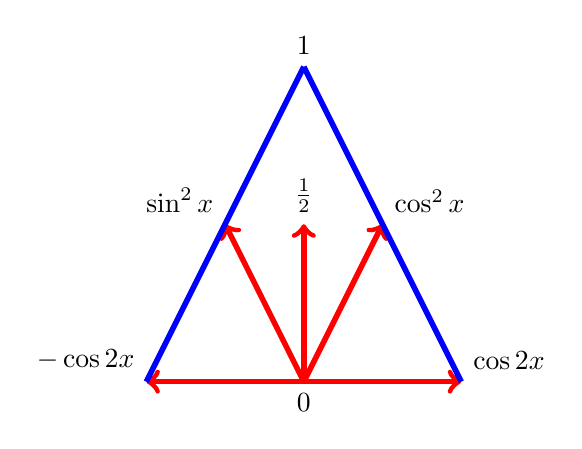
\begin{tikzpicture}[line width=2,scale=2]
			\draw[->,red] (0,0) -- (0,1);
			\draw[->,red] (0,0) -- (-1,0);
			\draw[->,red] (0,0) -- (1,0);
			\draw[->,red] (0,0) -- (1/2,1);
			\draw[->,red] (0,0) -- (-1/2,1);
			\draw[blue] (-1,0) -- (0,2);
			\draw[blue] (1,0) -- (0,2);
			
			\node[above left] (-cos2x) at (-1,0) {$-\cos 2 x$};
			\node[above right] (cos2x) at (1,0) {$\cos 2 x$};
			\node[above] (1/2) at (0,1) {$\frac{1}{2}$};
			\node[above] (1) at (0,2) {$1$};
			\node[above right] (cos^2x) at (1/2,1) {$\cos^2 x$};
			\node[above left] (sin^2x) at (-1/2,1) {$\sin^2 x$};
			\node[below] (0) at (0,0) {$0$};
		\end{tikzpicture} 
	\end{center} 
	An diesem Bild erkennt man verschiedene Zusammenhänge von $1, 1/2, \sin^2 x , \cos^2 x , \cos 2x$. Unter anderem sieht man auch die Basen des zweidimensionalen Vektorraums, der durch diese Vektoren aufgespannt ist: $1/2$ und $\cos 2 x$ bilden z.B. eine Basis, $\sin^2 x$ und $\cos^2 x$ bilden eine andere Basis. 
\end{bsp} 

\begin{defn}[Abstrakte Euklidische Räume über $\R$]
	Ein Vektorraum $V$ über $\R$, der mit einer Funktion $\sprod{\,.\,}{\,.\,} : V \times V \to \R$ ausgestattet ist, heißt \textbf{Euklidischer Raum} mit dem \textbf{Skalarprodukt} $\sprod{\,.\,}{\,.\,}$, wenn folgende Bedingungen erfüllt sind: 
	\begin{align*}
			\sprod{\alpha u + \beta v}{w} & = \alpha \sprod{u}{w} + \beta \sprod{v}{w} 
			\\ \sprod{u}{v} & = \sprod{v}{u}
			\\ \sprod{v}{v} & \ge 0 & \text{mit} \ \sprod{v}{v} & = 0  \Longleftrightarrow v =\mathbf{0}
	\end{align*} 
	Hierbei sind $u,v,w \in V$ und $\alpha,\beta \in \R$. Der Wert 
	\[
		\|u\| = \sqrt{ \sprod{u}{u} } 
	\]
	heißt die \textbf{Euklidische Norm} von $u$ und der Wert $\|u-v\|$ heißt der \textbf{Euklidische Abstand} von $u$ und $v$. Zwei Vektoren $u$ und $v$ heißen orthogonal, wenn $\sprod{u}{v}=0$ gilt. 
\end{defn} 

\begin{bem}
	Auch für Euklidische Räume gilt: neben den konkreten Räumen wie $\R^3$ mit  dem Skalarprodukt 
	\[
		\sprod{ \begin{pmatrix} u_1 \\ u_2 \\ u_3 \end{pmatrix} }{ \begin{pmatrix} v_1 \\ v_2 \\ v_3 \end{pmatrix} } = u_1 v_1 + u_2 v_2 + u_3 v_3,
	\]
	an die wir gewöhnt sind, kann man auch weitere Euklidische Räume betrachten. Analog zum Skalarprodukt 
	\[
		\sprod{u}{v} := \sum_{i=1}^n u_i v_i 
	\]
	für Vektoren $u= (u_i) , v = (v_i) \in \R^n$ des Raums $\R^n$ kann man auch das Skalarprodukt 
	\[
			\sprod{f}{g} := \int_0^T f(x) g(x) \dd x
	\]
	auf geeigneten Räumen von $T$-periodischen Funktionen einführen. 
\end{bem} 

\begin{defn}
	Eine System $u_i \ (i \in I)$ von Vektoren aus einem Euklidischen Raum $V$ heißt \textbf{Orthogonalsystem}, wenn alle $u_i$ ungleich $\textbf{0}$ sind und für alle $i,j \in I$ mit $i \ne j$ die Bedingung $\sprod{u_i}{v_j} = 0$ gilt. Gilt für ein Orthogonalsystem $\|u_i\|=1$ für alle $i \in I$, so nennt man es ein \textbf{Orthonormalsystem}. 
\end{defn} 

\begin{bem}
	Jedes Orthogonalsystem ist linear unabhängig. 
\end{bem} 

\begin{defn}
	Der Begriff einer Orthogonalbasis (bzw. Orhtononormalbasis) wird in der Theorie von unendlich-dimensionalen Vektorräumen oft folgendermaßen erweitert: man nennt ein Orthogonalsystem (bzw. Orthonormalsystem) $u_i$ ($i \in I$) von Vektoren aus einem Euklidischen Raum $V$ eine \textbf{Orthogonalbasis} (bzw. \textbf{Orthonormalbasis} von $V$, wenn jeder Vektor $v \in V$ beliebig gut durch eine endliche Linearkombination der Vektoren $u_i$ approximiert werden kann. Das heißt, für jedes $\epsilon>0$ gilt 
	\[
			\| v - (\alpha_1 u_{i_1}+ \cdots + \alpha_n u_{i_n})\| < \epsilon
	\] für endlich viele Indizes $i_1,\ldots,i_t \in I$ und $\alpha_1,\ldots,\alpha_n \in \R$. Im Folgenden werden wir diese Verallgemeinerung nutzen. 
\end{defn} 

\begin{bem}
	Im Fall von endlich-dimensionalen Euklidischen Räumen $V$ lassen sich die Orthogonal- und Orthonormalbasen einfacher beschreiben. Im Raum der Dimension $d \in \N$ ist eine Orthogonal- bzw. Orthonormalbasis ein Orthogonal- bzw. Orthonormalsystem $u_1,\ldots,u_d$ aus genau $d$ Vektoren. Jeder Vektor $v \in V$ kann direkt (ohne Approximation) als Linearkombination von Vektoren der Basis dargestellt werden. 
\end{bem} 

\begin{defn}
	Einen Vektorraum über $\R$, der eine Orthogonalbasis besitzt, nennt man einen (reellen) \textbf{Hilbertraum}.
\end{defn} 


\begin{bem}[Orthogonalbasen]
	Orthogonalbasen sind sehr praktisch. Ist $b_1,\ldots,b_d$ Orthogonalbasis eines Euklidischen Raums so kann man die Zerlegung
	\[
	f = \alpha_1 b_1 + \cdots + \alpha_d b_d
	\]
	für einen gegeben Vektor $f$ durch die Berechnung der Skalarprodukte bestimmen. Skalarmultiplikation mit $b_i$ ergibt 
	\[
	\alpha_i = \frac{ \sprod{f}{b_i} }{\sprod{b_i}{b_i}}
	\]
	Bei Orthonormalsystemen hat man $\sprod{b_i}{b_i} =1$. 
\end{bem} 

\begin{bem}[Der Satz des Pythagoras] Ist $f = \alpha_1 b_ 1+ \cdots \alpha_d b_d$ für ein Orthogonalsystem $b_1,\ldots,b_d$, so hat man 
	\[
		\|f\|^2 = \alpha_1 \|b_1\|^2 + \cdots + \alpha_d^2 \|b_d \|^2.
	\]
	Ist $b_1,\ldots,b_n$ ein Orthonormalsystem, so gilt 
	\[
		\|f\|^2 = \alpha_1^2 + \cdots + \alpha_d^2. 
	\]
\end{bem} 


\begin{thm}
	Ist $b_k$ $(k \in \N)$ eine Orthogonalbasis eines (reellen) Hilbertraums, so gilt für jeden Vektor $f \in V$  
	\[
			\lim_{n \to \infty} \left\| f - \sum_{i=1}^n \alpha_k b_k \right\| = 0
	\]
	mit 
	\[
		\alpha_k = \frac{\sprod{f}{b_k}}{\sprod{b_k}{b_k}}. 
	\]
	Darüber hinaus gilt
	\[
		\|f\|^2 = \sum_{k=1}^\infty \alpha_k^2 \|b_k\|^2. 
	\]
\end{thm} 

\begin{bem}
	Das vorige Theorem ist ein Analogon der Orthogonalbasiszerlegung und des Satzes von Pythagoraus für unendlich-dimensionale Euklidische Räume. 
\end{bem} 


\begin{aufg}
	Finden  Sie die Darstellungen von Vektoren in einer Basis:  
	\begin{enuma}
		\item  $v = \begin{pmatrix} 2 \\ 3 \end{pmatrix}$ in der Basis $b_1 = \begin{pmatrix} 1 \\ 1 \end{pmatrix}, b_2 =\begin{pmatrix} 1 \\ -1 \end{pmatrix}$
		\item 
	$v = \begin{pmatrix} 2 \\ 3 \\ 5 \\ 7 \end{pmatrix}$ in der Basis 
	$
			b_1 = \begin{pmatrix} 1 \\ 1 \\ 1 \\1 \end{pmatrix}, 
			b_2 = \begin{pmatrix} 1 \\ -1 \\ 1 \\-1 \end{pmatrix},
			b_3 = \begin{pmatrix} 1 \\ 1 \\ -1 \\-1 \end{pmatrix}, 
			b_4 = \begin{pmatrix} 1 \\ -1 \\ -1 \\1 \end{pmatrix}.
	$
		\end{enuma} 
\end{aufg} 



\begin{defn}
	Sei $V$ Euklidischer Raum sei $f \in f$ und sei $(f_k)_{k \in \N}$ eine Folge von Elementen aus $V$. Dann sagt man, dass $f_k$ gegen $f$ in der Norm konvergiert, wenn $\lim_{k \to \infty} \|f - f_k\| =0$ gilt. 
\end{defn} 

\begin{defn}
	Sei $V$ Euklidische Raum. Eine Reihe mit Elementen aus $V$ ist ein Ausdruck der Form $\sum_{k=1}^\infty g_k$ mit $g_k \in V$ für alle $k \in \N$. Man sagt, dass die Reihe gegen ein $f \in V$ in der Norm konvergiert, wenn 
	\[
			\lim_{n \to \infty} \| f - \sum_{k=1}^n g_k\| = 0
	\]
	gilt. In diesem Fall schreiben wir 
	\[
			f = \sum_{k=1}^\infty g_k. 
	\]
\end{defn} 

\section{Der Raum $\cL^2(0,T)$}

\begin{defn} 
	Wir führen den Vektorraum $\cL^2(0,T)$ ein, als den $\R$-Vektorraum aller $T$-periodischen Funktionen $f : \R \to \R$, die auf $[0,T]$,  Lebesgue-integrierbar sind, und die Bedingung
	\[
		\int_0^T |f(x)|^2 \dd x < +\infty. 
	\]
	erfüllen. 
	In diesem Raum führen wir das Skalarprodukt 
	\[
		\sprod{f}{g}_{\cL^2(0,T)} = \int_0^T f(x) g(x) \dd x 
	\]
	ein und die zugehörige Norm 
	\[
		\|f \|_{\cL^2(0,T)} :=  \sqrt{ \int_0^T f(x)^2 \dd x}.
	\]
	Zwei Funktionen $f, g \in \cL^2(0,T)$ werden identifiziert, wenn man $\|f-g\|_{\cL^2(0,T)}=0$ hat. Das ist z.B. der Fall, wenn sich $f$ und $g$ innerhalb von $[0,T]$ nur in endlich vielen Stellen unterscheiden. 
\end{defn} 

\begin{bem}
	In der vorigen Definition benutzen wir das Lebesgue-Integral, das wir in diesem Kurs gar nicht eingeführt haben. Das ist für uns kein Problem: für die Beispiele, die wir betrachten, reicht die Theorie der Riemann-Integrale aus.
\end{bem} 


\begin{thm}
	Die Funktionen des Systems
	\begin{align}
		\label{fourier:system}
		 \frac{1}{2}, \ \cos  \omega x, \cos 2 \omega x, \cos 3\omega x, \ldots , \ \sin  \omega x, \sin 2 \omega x, \sin 3 \omega x, \ldots 
	\end{align}
	bilden eine Orthogonalbasis für den Raum $\cL^2(0,T)$ mit $T = \frac{2 \pi}{\omega}$. 
\end{thm} 	

\begin{aufg} 
	Verifizieren Sie, dass \eqref{fourier:system} tatsächlich ein orthogonales System bilden. Berechnen Sie auch die $\cL^2(0,T)$-Norm jeder Funktion aus \eqref{fourier:system}.
\end{aufg} 



\section{Formeln für die Koeffizienten}

\begin{bem}[Formeln für die Koeffizienten der Fourier-Reihe] 
	Für
	\[
		f(x) = \frac{a_0}{2} + \sum_{k=1}^\infty (a_k \cos k \omega x + b_k \sin k \omega x) \in \cL^2(0,T)
	\]
	mit $T = \frac{2 \pi}{\omega}$
	gilt  
	\begin{align*}
		a_k & = \frac{2}{T} \int_0^T f(x) \cos k \omega x \dd x & & (k=0,1,2\ldots),
	\\	b_k & = \frac{2}{T} \int_0^T f(x) \sin k \omega x \dd x & & (k=1,2,\ldots).
	\end{align*}
\end{bem} 

\begin{bem}[Formeln für die Koeffizienten der Fourier-Reihe im Fall $\omega =1$] 
	Für
	\[
	f(x) = \frac{a_0}{2} + \sum_{k=1}^\infty (a_k \cos k x + b_k \sin k x) \in \cL^2(0,2 \pi)
	\]
	gilt  
	\begin{align*}
	a_k & = \frac{1}{\pi} \int_0^{2\pi} f(x) \cos k  x \dd x & & (k=0,1,2\ldots),
	\\	b_k & = \frac{1}{\pi} \int_0^{2 \pi} f(x) \sin k x \dd x & & (k=1,2,\ldots).
	\end{align*}
\end{bem} 

\begin{aufg}[Realitätscheck] 
	Was sind die Fourier-Entwicklungen von $\sin x$, $\cos 2x$ und $2 \sin x - \cos 2x$? Muss man integrieren, ob diese Entwicklungen zu bestimmen? 
\end{aufg} 


\begin{bem}[Tipps und Tricks]
	Man beachte dass $\cos x$ eine gerade und $\sin x$ eine ungerade Funktion ist. Das hat die folgenden Auswirkungen auf die Entwicklung in die Fourier-Reihe: 
	\begin{enuma}
		\item $f$ gerade, d.h., $f(x) = f(-x)$ für alle $x \in \R$ $\Longrightarrow$ alle $b_k$ gleich $0$. 
		\item $f$ ungerade, d.h., $f(x) = -f(-x)$ für alle $x \in \R$ $\Longrightarrow$ alle $a_k$ gleich $0$. 
	\end{enuma} 
\end{bem} 

\begin{bsp}
	Sei $f(x)$ die Funktion mit $f(x) = x- \pi$ für $0 < x < 2 \pi$, die wir $2\pi$-periodisch auf $\R$ erweitern. Da $f$ ungerade ist, gilt 
\[
 f (x)  = \sum_{k=1}^\infty b_k \sin k x. 
\]
Die Koeffizienten:
\begin{align*}
b_k = \frac{1}{\pi} \int_0^{2 \pi} (x-\pi) \sin k x \dd x = \frac{1}{\pi} \int_0^{2 \pi} x \sin k x \dd x = - \frac{2}{k} 
\end{align*}
Approximation durch $\sum_{k=1}^{10} b_k \sin k x$: 
	\begin{center}
	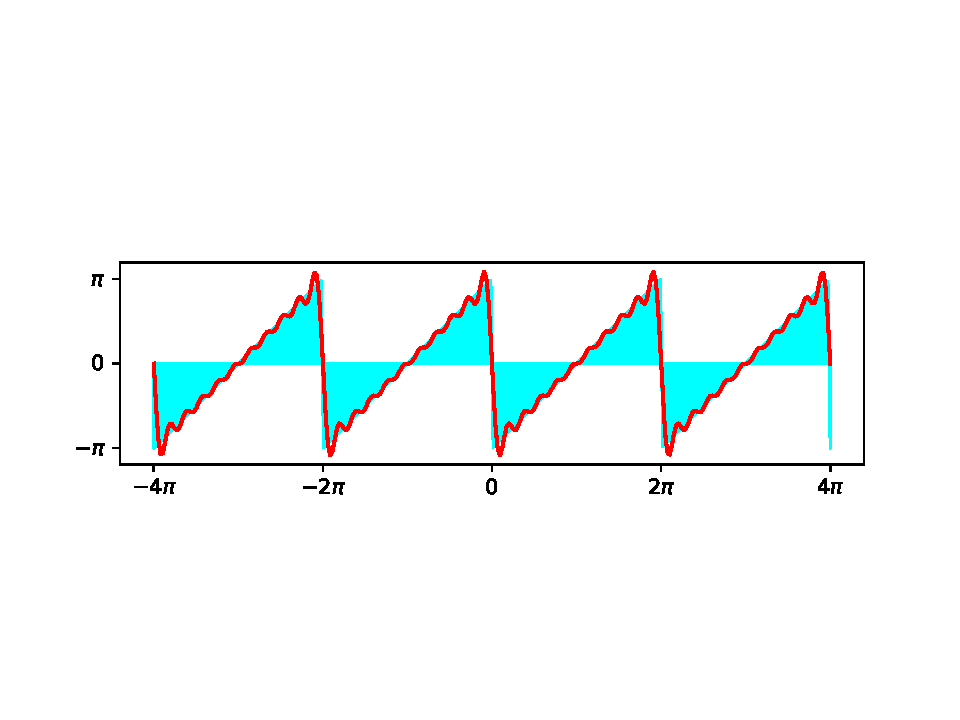
\includegraphics[width=0.8\textwidth]{pics/fourier.pdf}
\end{center}
\end{bsp} 

\begin{aufg} Berechnen Sie die Fourier-Entwicklung folgender Funktionen: \label{aufg:fourier:sin:cos:etc}
	\begin{enuma}
		\item $f = \sign (\cos (x))$
		\item $g = \sin x \cos x$
		\item $f+g$
		\item $h = \cos^4 x$
		\item $f(x+\pi/4)$
	\end{enuma} 
\end{aufg} 

\begin{aufg} 
	Nehmen wir an, Sie haben die Fourier-Entwicklung einer Funktion $f(x) \in \cL^2(0,2 \pi)$ ausgerechnet. Wie kann man daraus die Fourier-Entwicklung von $f(x+\alpha)$ für ein gegebenes $\alpha \in \R$ bestimmen? Geben Sie die Formeln für die Koeffizienten $\tilde{a}_0, \tilde{a}_1, \tilde{a}_2,\ldots, \tilde{b}_1,\tilde{b}_2,\ldots$ der Fourier-Entwicklung von $f(x+\alpha)$ in Abhängigkeit von den Koeffizienten $a_0,a_1,a_2,\ldots, b_1,b_2,\ldots$ der Fourier-Entwicklung von $f(x)$. 
	Wie hängen $\tilde{a}_k^2 + \tilde{b}_k^2$ und $a_k^2  + b_k^2$ für $k \in \N$ zusammen? 
\end{aufg} 

\begin{aufg} 
	Seien $f $ und $g$ die $2\pi$-periodische Funktionen mit 
	\begin{align*}
			f(x) & = x^2 & & \text{für} \ x \in [-\pi,\pi]
			\\ g(x) & = x^2 & & \text{für} \ x \in [0,2 \pi). 
	\end{align*} 	
Zeichnen Sie die Graphen dieser Funktionen auf dem Interval $[-3\pi,3\pi]$. Berechnen Sie die Fourier-Entwicklungen der beiden Funktionen. Welche Wahl der Integrationsbereiche ist bei Berechnung der Fourier-Koeffizienten günstig? 
\end{aufg} 

\begin{aufg}
	Man betrachte $2\pi$-periodische Funktionen $f$ und $g$ mit 
	\[
			f(x):= 
			\begin{cases}
				1 & x \in [0,\pi]
				\\ 0 & x \in [\pi,2\pi) 
			\end{cases} 
	\]
	und 
	\[
			g(x) := 
			\begin{cases}
					0 & x \in [0,\pi]
					\\1 & x \in (\pi,2\pi).  
			\end{cases} 
	\]
	Berechnen Sie die Fourier-Entwicklung von $f, g$ und $f + 2 g$. Vgl. diese Aufgabe mit  Aufgabe~\ref{aufg:fourier:sin:cos:etc}(a). 
\end{aufg} 

\section{Differenzieren von Fourier-Reihen} 

	\begin{thm} \label{thm:diff:f:reihe} 
		Sei $f$ die $2\pi$-periodische Erweiterung einer differenzierbaren Funktion $g : \R \to \R$ mit $g(0) = g(2\pi)$. Wenn $f$ und $f'$ zu $\cL^2(0,2\pi)$ gehören, dann ergibt sich die Fourier-Entwicklung von $f'$ durch gliederweise Differenzieren der Fourier-Entwicklung von $f$. 
		
		Mit anderen Worten: unter den genannten Voraussetzungen an $ f = \frac{a_0}{2} + \sum_{k=1}^n (a_k \cos k x + b_k \sin k x)$ gilt 
		\[
				\left( \frac{a_0}{2} + \sum_{k=1}^\infty (a_k \cos k x + b_k \sin k x) \right)' = \sum_{k=1}^n (a_k \cos k x + b_k \sin k x)'. 
		\]
	\end{thm} 

\begin{bem}[Begründung] 
	Wir betrachten die beiden Fourier-Entwicklungen: 
	\begin{align*}
		f(x) & = \frac{a_0}{2}  + \sum_{k=1}^\infty (a_k \cos k x + b_k \sin k x),
		\\ f'(x) & = \frac{a_0'}{2} + \sum_{k=1}^\infty (a_k' \cos k x + b_k' \sin k x).
	\end{align*} 
	Man hat 
	\begin{align*}
		a_k' & = \frac{1}{\pi} \int_0^{2\pi} f'(x) \cos k x \dd x & & |\text{ Formeln für die Koeffizienten} 
		\\ & = \underbrace{\biggl[ f(x) \cos k x \biggr]_{x=0}^{2 \pi}}_{=0} - \frac{1}{\pi} \int_0^{2 \pi} f(x) (\cos k x)' \dd x & & |\text{ Partielle Integration}
		\\ & = \frac{k}{\pi} \int_0^{2 \pi} f(x) \sin k x \dd x & & 
	\end{align*} 
	Also ist $a_0' = 0$ und $a_k' = k b_k$ für $k \in \N$. 
		
	Analog zeigt man auch $b_k' = -k a_k$ für $k \in \N$. Das führ zur Formel: 
	\[
		f'(x) = \sum_{k=1}^\infty (a_k \cos k x + b_k \sin k x)'. 
	\]
\end{bem} 

\begin{bsp} 
	Wir erweitern $f(x) = (x-\pi)^2 $ periodisch von $[0,2\pi]$ auf $\R$. Da wir die Funktion $x-\pi$ auf $[0,2 \pi)$ bereits in die Fourier-Reihe entwickelt haben, wissen wir, dass man für $f'(x) = 2 (x-\pi)$ die Entwicklung 
	\[
		f'(x)  = - 4 \sum_{k=1}^\infty \frac{\sin k x}{k} 
	\]
	Nun können wir darauf basierend die Entwicklung 
	\[
		f(x) = \frac{a_0}{2} + \sum_{k=1}^\infty (a_k \sin k x  + b_k \cos k x)
	\] 
	bestimmen. Das Differenzieren dieser Entwicklung gliederweise gibt uns die Entwicklung von $f'(x)$. Daraus lassen sich die Koeffizienten $a_k$ und $b_k$ für alle $k \in \N$ bestimmen. Wir erhalten 
	\[
		f(x) = \frac{a_0}{2} + 4 \sum_{k=1}^\infty \frac{\cos k x}{k^2}. 
	\]
	Zur Berechnung des Koeffizienten $a_0$ können wir die Standard-Formel 
	\[
		a_0 = \frac{1}{\pi} \int_0^{2 \pi}	f(x) \dd x
	\]
	benutzen. Wir erhalten
	\[
		f(x) = \frac{\pi^2}{3} + 4 \sum_{k=1}^\infty \frac{ \cos k x}{k^2}. 
	\]
\end{bsp} 

\begin{bem}
	{\color{red} Warnung!} Beim Anwenden von Theorem~\ref{thm:diff:f:reihe} sollen die Voraussetzungen beachtet werden! Theorem~\ref{thm:diff:f:reihe} ist für unstetige $2\pi$-periodische Funktionen $f : \R \to \R$ \textbf{nicht} anwendbar. 
\end{bem} 

\section{Pythagoras in $\cL^2(0,T)$}

\begin{bem}
	Wenn wir zwei Funktionen $f_1(x), f_2(x) \in \cL^2(0,2 \pi)$ haben: 
	\[
		f_s(x) = \frac{a_{s,0}}{2} + \sum_{k=1}^\infty (a_{s,k} \cos k x + b_{s,k} \sin k x) \in \cL^2(0,2 \pi),
	\]
	so gilt 
	\[
		\underbrace{\int_0^{2\pi} f_1(x) f_2(x) \dd x}_{\text{Skalarprodukt von Funktionen}} = \sprod{f_1}{f_2}_{\cL^2(0,2\pi)} = \pi \underbrace{\left( \frac{1}{2} a_{1,0} a_{2,0} + \sum_{k=1}^\infty (a_{1,k} a_{2,k} + b_{1,k} b_{2,k})\right)}_{\substack{\text{ein Skalarprodukt von zwei Folgen} \\ \text{ von Fourier-Koeffizienten}}}
	\]
	
	Im Fall $f_1=f_2=f$ erhalten wir\ldots 
\end{bem} 

\begin{thm}[Parseval'sche Gleichung]
	Für 
	\[
		f(x) = \frac{a_0}{2} + \sum_{k=1}^\infty (a_k \cos k x + b_k \sin k x) \in \cL^2(0,2 \pi). 
	\]
	gilt
	\[
		\|f \|_{\cL^2(0,2 \pi)}^2 = \int_0^{2 \pi} f(x)^2 \dd x =\pi \left( \frac{a_0^2}{2} + \sum_{k=1}^\infty (a_k^2 + b_k^2 ) \right).
	\]
\end{thm} 

\begin{bem} Parseval'sche Gleichung ist der Satz von Pythagoraus in unendlich vielen Dimensionen. 
\end{bem} 

\begin{bsp}
	Wir berechnen $\sum_{k=1}^\infty \frac{1}{k^2}$  mit Hilfe der Parseval'schen Gleichung. Wir wählen als $f(x)$ die Funktion mit $f(x) = x- \pi$ für $0 < x < 2 \pi$, die wir $2\pi$-periodisch auf $\R$ erweitern. Da $f$ ungerade ist, gilt 
	\[
		\int_0^{2 \pi} f(x)^2 \dd x = \pi \sum_{k=1}^\infty b_k^2.
	\]
	Die linke Seite ist 
	\[
		\int_0^{2 \pi} (x-\pi)^2 \dd x = \biggl[ \frac{(x-\pi)^3}{3} \biggr]_{x=0}^{2 \pi} = \frac{2 \pi^3}{3}. 
	\]
	Also gilt 
	\[
		\sum_{k=1}^\infty b_k^2 = \frac{2 \pi^2}{3}.
	\]
	Die Koeffizienten $b_k$ sind 
	\begin{align*}
		b_k = \frac{1}{\pi} \int_0^{2 \pi} (x-\pi) \sin k x \dd x = \frac{1}{\pi} \int_0^{2 \pi} x \sin k x \dd x = - \frac{2}{k} 
	\end{align*}
	Das ergibt: 
	\[
		\sum_{k=1}^\infty \left( \frac{2}{k} \right)^2 = \frac{2 \pi^2}{3}
	\]
	und somit 
	\[
		\sum_{k=1}^\infty \frac{1}{k^2}  = \frac{\pi^2}{6}.
	\]
\end{bsp} 

\section{Fourier-Reihen für komplexwertige Funktionen} 

\begin{bem}
	Vgl. lineare Algebra bzgl. der Definition der Euklidischen Räume über $\C$. Orthogonal- und Orthonormalbasen für Vektorräume über $\C$ können analog definiert werden. Ein komplexer Hilbertraum ist ein (endlich oder unendlich-dimensionaler) Euklidischer Raum über $\C$, der eine Orthogonalbasis besitzt. 
\end{bem} 

\begin{bem}
	Wegen der Euler-Formel sind wir motiviert $e^{\iu k x}$ mit $k \in \Z$ als die Basis der Fourier-Entwicklung zu nutzen. Dementsprechend müssen wir 
\end{bem}


\begin{bem} 
	Oft arbeitet  man auch mit komplexwertigen $T$-periodischen Funktionen $ f: \R \to \C$. In diesem Fall definiert man $\cL^2(0,T)$ entsprechend als einen $\C$-Vektorraum mit 
	\[
	\sprod{f}{g}_{\cL^2(0,T)} = \int_0^T f(x) \overline{ g(x) } \dd x 
	\]
	und 
	\[
	\|f \|_{\cL^2(0,T)} := \sqrt{ \int_0^T |f(x)|^2 \dd x}.
	\]
	Das bedeutet, dass man den Euklidischen Raum $\cL^2(0,T)$ über $\R$ zu einem entsprechenden Raum über $\C$ erweitert. Wir benutzen die selbe Bezeichnung für diesen größeren Raum. 
\end{bem} 


\begin{bem}
	Das System $\bigl( e^{\iu k x} \bigr)_{k \in \Z}$
	ist die Standardwahl einer Orthogonalbasis für den Vektorraum $\cL^2(0,2 \pi)$ (über $\C$). Man definiert die Fourier-Entwicklung dazu als: 
	\[
		f(x) = \sum_{k=-\infty}^{\infty} c_k e^{\iu k x}.
	\]
	Diese Gleichung interpretiert man als den Grenzwert
	\[
		\lim_{n \to \infty} \left\| f(x) -   \sum_{k=-n}^{n} c_k e^{\iu k x}\right\|_{\cL^2(0,2 \pi)}  = 0.
	\]
	Die Formel für die Koeffizienten: 
	\[
		c_k = \frac{1}{2\pi} \int_0^{2\pi} f(x) e^{-\iu k x} \dd x. 
	\]
\end{bem} 

\begin{bsp} 
	Wir berechnen die Fourier-Entwicklung der Funktion
	\[
		f(x) := \begin{cases} 1, & 0 \le x < \pi \\
		0, & \pi \le x < 2 \pi, \end{cases},
	\]
	die auf  die gesamte reelle Achse $2\pi$-periodisch erweitert wird, in der ``exponentiellen Basis'' $(e^{\iu k x})_{k \in \Z}$ und anschließend in der ``trigonometrischen Basis''. Man hat 
	\[
		c_0 = \frac{1}{2 \pi} \int_0^{2 \pi} f(x) \dd x = \frac{1}{2}. 
	\]
	Für $k \in \Z \setminus \{0\}$ hat man 
	\begin{align*}
		c_k & = \frac{1}{2 \pi} \int_0^{2 \pi }	f(x) e^{-\iu k x} \dd x
		\\ & = \frac{1}{2 \pi} \int_0^{\pi} e^{-\iu k x} \dd x 
		\\ & = \biggl[ \frac{\iu}{2 \pi k}  e^{-\iu k x} \biggr]_{x=0}^{\pi}. 
		\\ & = \frac{\iu }{2\pi k} ( e^{-\iu k \pi } -1). 
		\\ & = \begin{cases} - \frac{\iu}{\pi k} & k \ \text{ungerade} , 
		\\ 0 & k \ \text{gerade} \end{cases} 
	\end{align*}
	Das ergibt die Entwicklung 
	\[
		f(x) = \frac{1}{2} - \frac{\iu}{\pi} \sum_{\ell = - \infty}^\infty \frac{1}{2 \ell +1} e^{\iu (2\ell+1) x}
	\]
	in der exponentiellen Basis. 
	Um die Entwicklung in der trigonometrischen Basis zu erhalten, werden die  Glieder in Paare zerlegt, sodass $e^{\i k x}$ und $e^{-\iu k x}$ in ein neues Glied aufgenommen werden, das als Summe von zwei Gliedern der vorigen Entwicklung entsteht. 
	\[
		f(x) = \frac{1}{2} - \frac{1}{\pi} \sum_{m=1}^{+\infty} \frac{1}{2m -1} \iu \bigl(e^{\iu (2m-1) x} - e^{- \iu (2m-1) x} \bigr). 
	\]
	Durch die Anwendung der Euler-Formel erhalten wir nun auch die Darstellung
	\[
		f(x) = \frac{1}{2}  +\frac{2}{\pi} \sum_{m=1}^\infty \frac{\sin (2m-1) x } {2m-1}
	\]
	in der trigonometrischen Basis. (Diese Darstellung kann man natürlich auch direkt erhalten.) 
\end{bsp} 

\begin{bem}[Pythagoras]
	Für zwei Funktionen $f_1, f_2 \in \cL^2(0,2\pi)$ mit 
	\[
		f_s(x) = \sum_{k=-\infty}^\infty c_{s,k} e^{\iu k x}
	\]
	gilt 
	\[
		\int_0^{2 \pi} f_1(x) \overline{f_2(x))} \dd x = \sprod{f_1}{f_2}_{\cL^2(0,2 \pi)} = 2 \pi \underbrace{ \sum_{k=-\infty}^\infty c_{1,k} \overline{c_{2,k}} }_{\substack{\text{ein Skalarprodukt von zwei} \\ \text{komplexwertigen Folgen}}}. 
	\]
	Insbesondere hat man im Fall $f=f_1 =f_2$: 
	\[
		\int_0^{2 \pi} |f(x)|^2 \dd x = 2 \pi \sum_{k=-\infty}^\infty |c_k|^2.
	\]
\end{bem} 

\begin{bem} 
	Der Raum $\cL^2(0,\pi)$ ist also isometrisch zum komplexen Euklidischen Raum $\ell^2$ aller Folgen $c = (c_k)_{k \in \Z}$ mit $c_k \in \C$ und mit 
	der Eigenschaft 
	\[
		\sum_{k = -\infty}^\infty |c_k|^2 < \infty. 
	\]
	Die Norm in diesem Raum ist: 
	\[
		\|c\|_{\ell^2} := \sqrt{ \sum_{k = -\infty}^\infty |c_k|^2 }.  
	\]
	Das Skalarprodukt zu dieser Norm ist: 
	\[
		\sprod{c}{d} = \sum_{k=-\infty}^\infty c_k \overline{d_k} 
	\]
	für $c = (c_k)_{k \in \Z}, d = (d_k)_{k \in \Z}  \in \ell^2$. 
\end{bem} 

\begin{bem}[Übergang von der Exponentialbasis zur trigonometrischen Basis]
	\[
		f(x) = \sum_{k=-\infty}^\infty c_k e^{\iu k x} = \frac{a_0}{2} +  \sum_{k=1}^\infty (a_k \cos k x + b_k \sin k x). 
	\]
	Man hat 
	\[
		a_0 = 2 c_0
	\]
	und, nach der Euler-Formel, 
	\[
		c_k \underbrace{(\cos k x + \iu \sin k x)}_{=e^{\iu kx}} + c_{-k} \underbrace{(\cos k x - \iu \sin k x)}_{=e^{-\iu kx}} = a_k \cos k x + b_k \sin k x
	\]
	für $k \in \N$. 
	
	Also gilt
	\begin{align*}
		a_k & = c_k + c_{-k} 
	\\	b_k & = \iu (c_k - c_{-k}) 
	\end{align*}
	für $k \in \N$. 
\end{bem} 

\begin{bem}[Übergang von ``trigonometrischen Basis'' zur ``Exponentialbasis'']
	\[
		c_0 =\frac{a_0}{2}.
	\]
	Für $k \in \N$ gilt: 
	\begin{align*}
		c_k & = \frac{ a_k - \iu b_k }{2}
	\\	c_{-k} & = \frac{a_k + \iu b_k}{2} 
	\end{align*}
\end{bem} 



\section{Die Verwandten der Fourier-Reihe} 

\begin{bem}[Diksrete Fourier-Transformation (=DFT)]
Analog zu Stetigen periodischen Funktionen auf $\R$ kann man $n$-Periodische Funktionen auf $\Z$ betrachten. Die Diskrete Fourier-Transformation (DFT) ist eine Art Fourier reihe für solche Funktionen.
\end{bem} 

\begin{bem}[Diskrete harmonische Funktionen und `diskrete Fourier-Reihen']
	Den analogen harmonischen Funktionen $e^{\iu k x}$ entsprechen in der Welt der $n$-periodischen diskreten Signale die Folgen
	\[
		p_k := \bigl( e^{\frac{2 \pi \iu k j}{n}} \bigr)_{j \in \Z}
	\]
	für $k \in \{0,\ldots,n-1\}$. Ein $n$-periodisches Signal $f = (f_j)_{j \in \Z}$ kann man mit dem Vektor $(f_j)_{j=0,\ldots,n} \in \C^n$ identifizieren, weil es ausreicht die Werte, in einer Periode zu notieren. 
	
	Die Zerlegung von $f = (f_j)_{j=0,\ldots,n} \in \C^n$ in harmonische Signale ist somit eine Darstellung der Form 
	\begin{equation}
	\label{diskrete:fourier:reihe}
	f_j = \sum_{k=0}^{n-1} e^{\frac{2 \pi \iu j k}{n}} c_k 
	\end{equation}
	mit $j=0,\ldots,n-1$ und $c=(c_k)_{k=0,\ldots,n-1} \in \C^n$. 
\end{bem}

\begin{bem}
	Bei der digitalen Darstellung eines Signals fixiert man die Sampling Rate $r$ (etwa in Frames Per Sekunde). Ist $i$ der Index des Frames so ist die Zeit $t = i / r$ der Zeitpunkt, in dem dieser Frame beim Abspielen dran ist. Den reine (Sinus)Ton mit der Frequenz $\nu$ hat die Form 
	\[
			\sin ( 2\pi \nu   t) = \sin ( \frac{2 \pi \nu}{r} i).  
	\]
	Die typische Wahl der Sampling Rate bei Audioaufzeichnungen ist $44100$ und $48000$ Frames pro Sekunde. 
	Den Standard-Kammerton (den A-Ton) hat man für $\nu = 440$ Hz. Ist $N$ die Anzahl der Frames, so dauert die Wiedergabe $N/ r$ Sekunden. Der folgende Code spielt eine Sekunde lang den Standard-Kammerton ab: 
\begin{lstlisting}[language=Python]
import sounddevice as sd
from math import * 
r=48000
nu=440
a=[sin(2*pi*nu*i/r) for i in range(r)]
sd.play(a,r)
\end{lstlisting}
Die diskrete Fourier-Transformation ermöglicht einem, aus einer Aufzeichnung, die Amplituden und Phaen der Töne, aus denen die Aufzeichnung zusammengesetzt ist,  abzulesen. Mit diesem Code kann man ein Signal mit der Dauer von $2$ Sekunden vom Mikrofon aufzeichnen. 
\begin{lstlisting}[language=Python]
a=sd.rec(2*r,r,1)
\end{lstlisting}
% the version sd.rec(2*r,r,1,blocking=True) should wait until the signal is recorded
\end{bem} 

\begin{bsp} Mit diesem Code sieht man, wie man anhand des gegebenen Signals mit Hilfe der Fourier-Transformation die Frequenzen bestimmt, aus denen das Signal besteht: 
\lstinputlisting{code/fft_audio_signal.py} 
Hier ein Ausschnitt eines Signals: 
\begin{center}
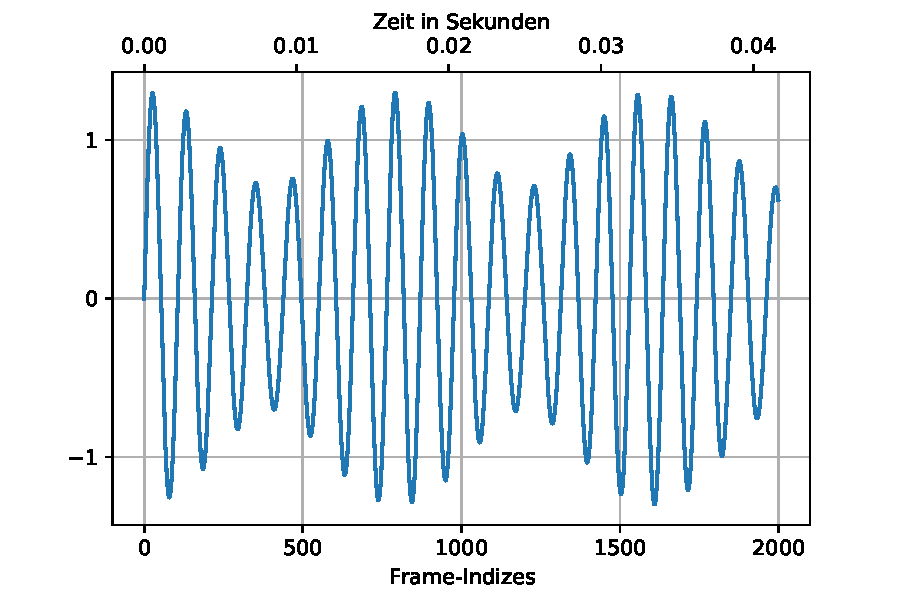
\includegraphics[width=0.5\textwidth]{code/combi_signal.pdf}
\end{center} 
Hier die Frequenzen, die im Signal identififizert wurden: 
\begin{center}
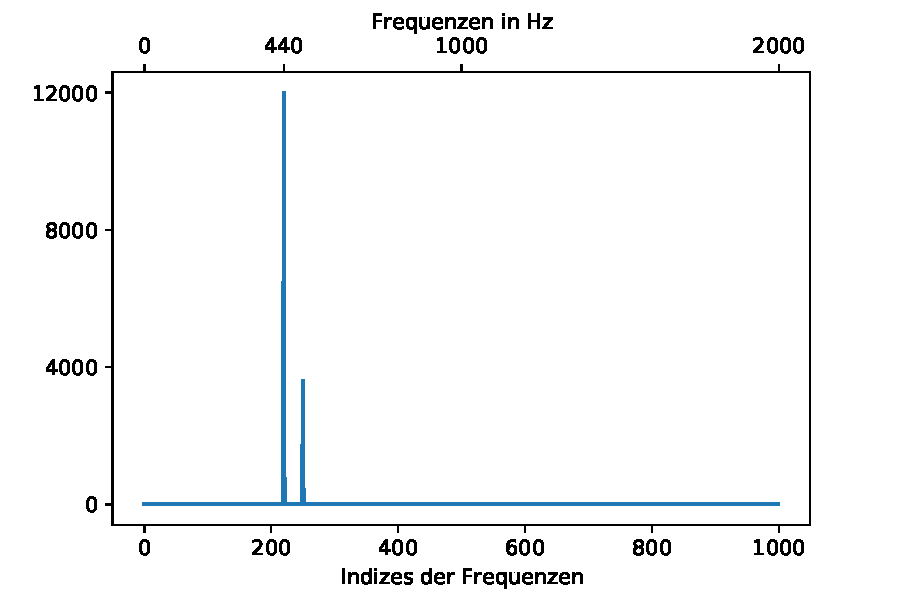
\includegraphics[width=0.5\textwidth]{code/combi_signal_fft.pdf}
\end{center} 
\end{bsp} 

\begin{bsp}
	Hier die Darstellung der komplexen harmonischen Funktionen. Der Realteil der harmonischen Funktionen wird in Blau und der Imaginärteil in Rot dargestellt. %Fall $n=8$:
	%\begin{center}
	%	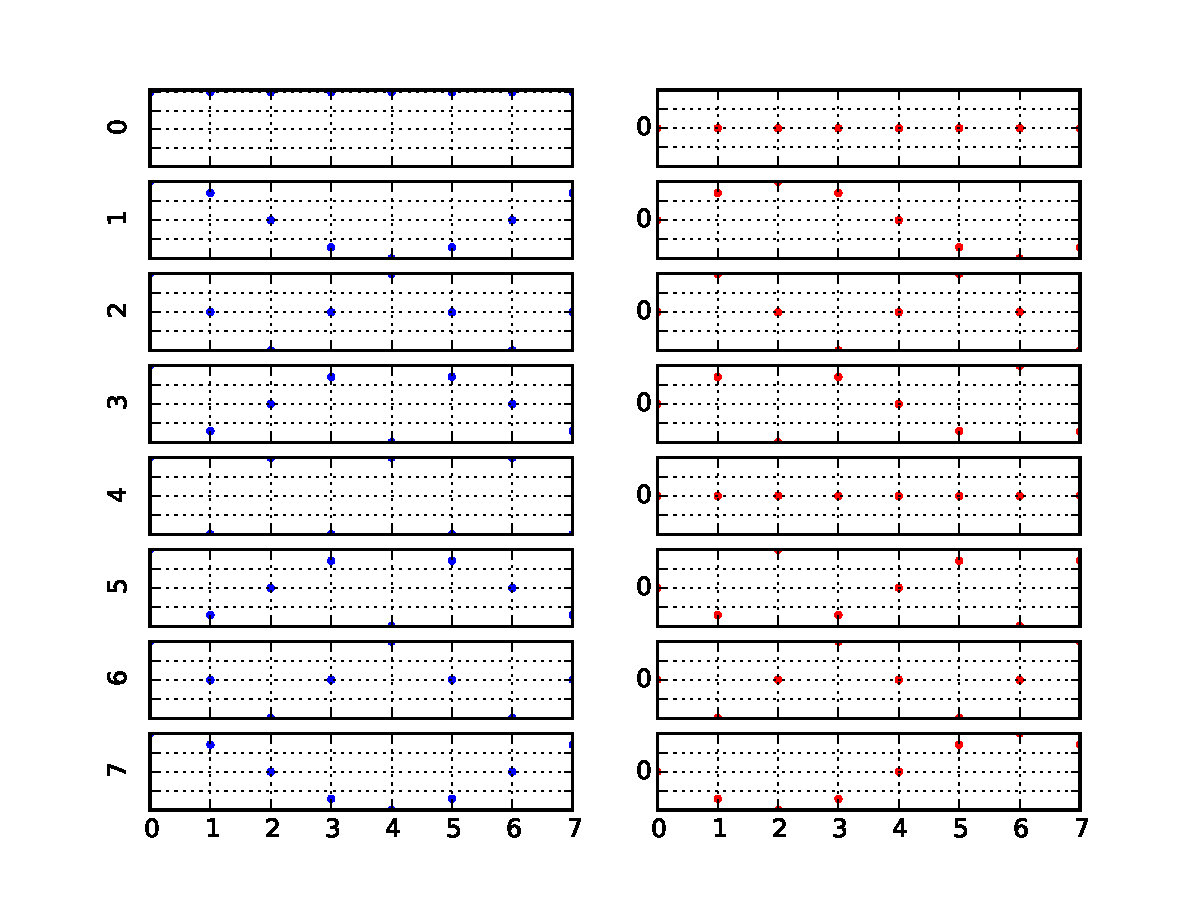
\includegraphics[width=20em]{pics/dft_harmonics_8.pdf}	
	%\end{center}
	%Fall $n=12$:
	%\begin{center}
	%	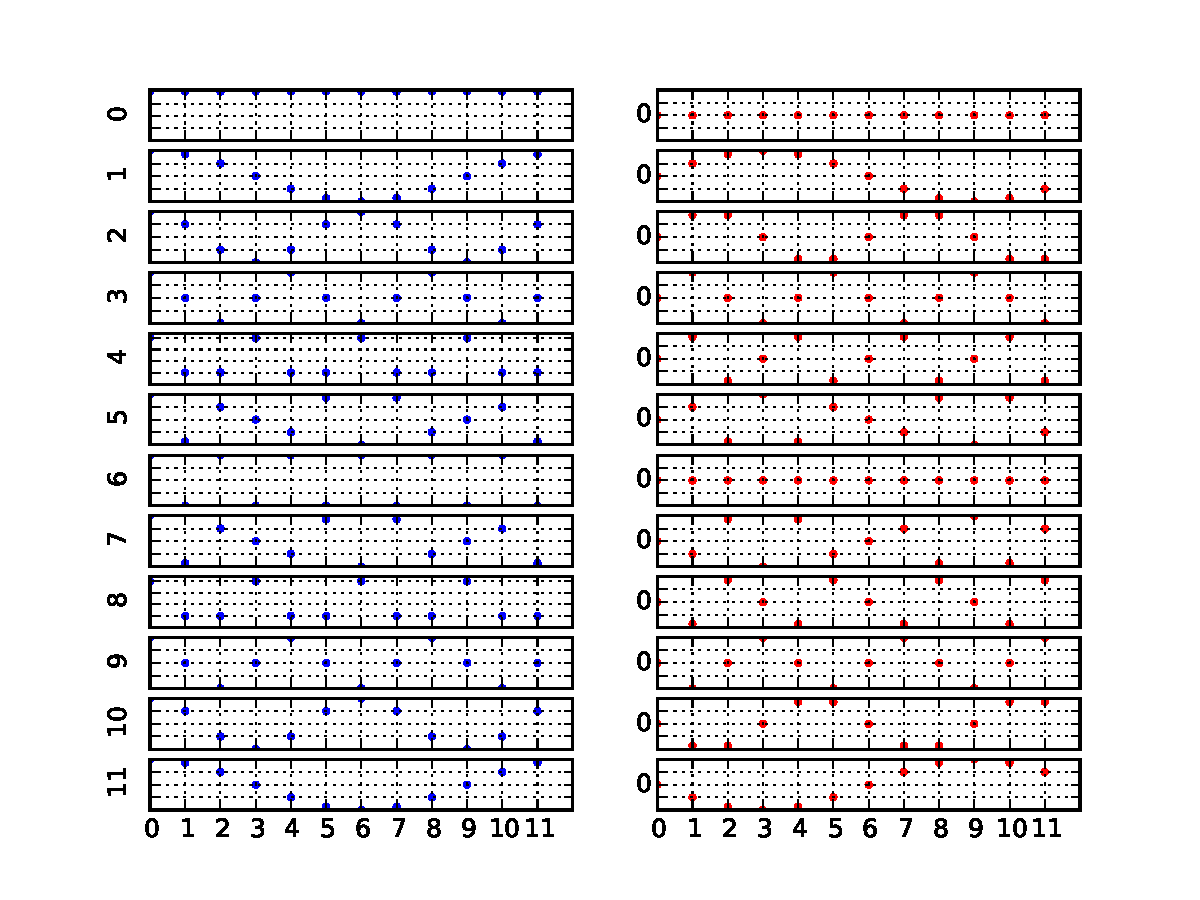
\includegraphics[width=30em]{pics/dft_harmonics_12.pdf}	
	%\end{center}
	Fall $n=16$:
	\begin{center}
		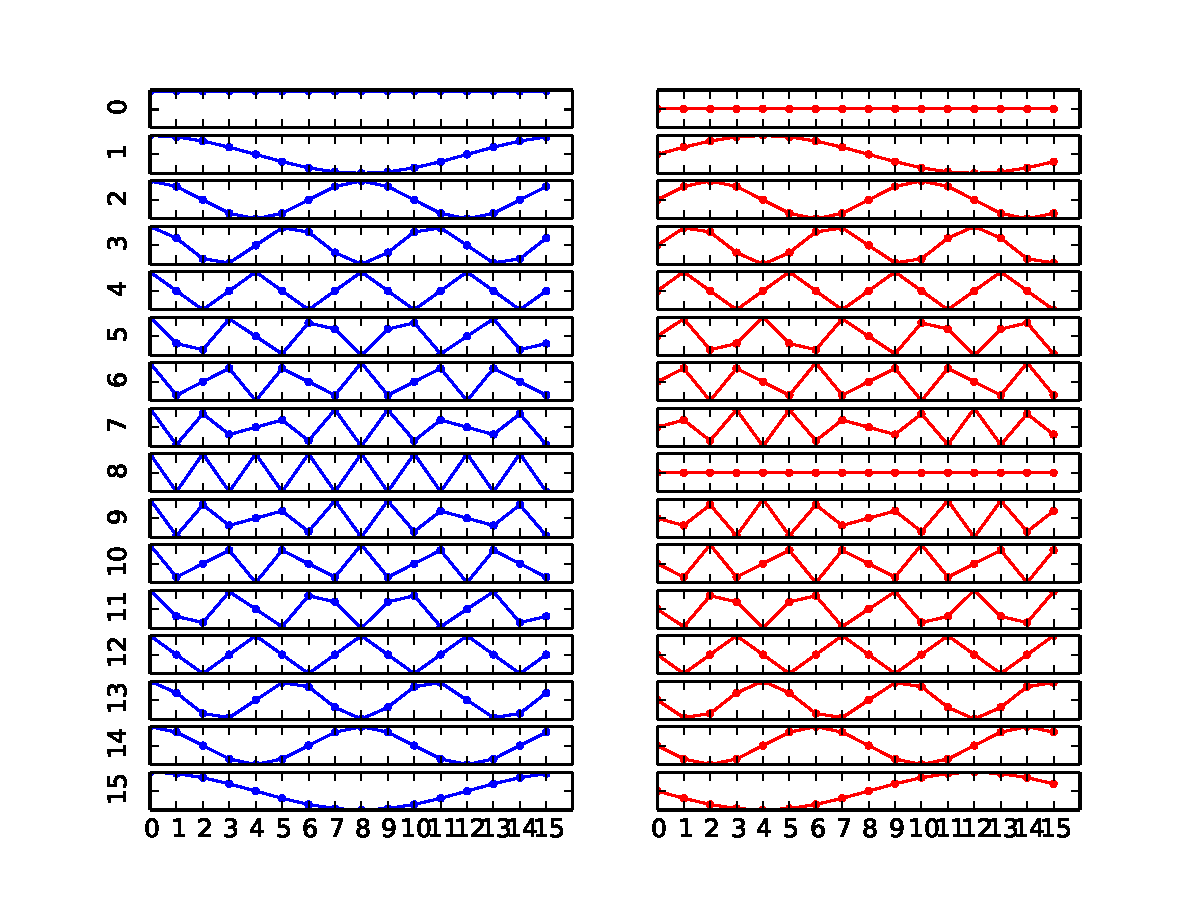
\includegraphics[width=30em]{pics/dft_harmonics_16.pdf}	
	\end{center}
	%Bei $n=16$ erkennt man in den harmonischen Funktionen mit Frequenzen $1$ und $2$ immer noch die Kosinus- und Sinusfunktionen. 
\end{bsp}

\begin{bem}
	FFT ($=$ Fast Fourier Transform) ist der schnelle Algorithmus zur Berechnung der DFT. In Matlab als die Funktion fft verfügbar. Hier ein Beispiel zum ``Entrauschen'' mit Hilfe der DFT: 
	\url{https://www.mathworks.com/help/matlab/ref/fft.html} 
\end{bem} 

\begin{bem}
		Fourier-Integrale: 
		\[
			f(x) = \int_{-\infty}^\infty c(\omega) e^{i \omega x} \dd x
		\]
		für $f : \R \to \C$ (hier muss $f$ nicht periodisch sein). 
		Im Gegenteil zu Fourier-Reihen ist hier das Spektrum (die Anzahl der Frequenzen in der Zerlegung) nicht mehr diskret. 
\end{bem} 

\begin{bem}
	Wenn man die Potenz-Reihen in einer komplexen Variablen $z \in \C$ betrachtet, kann man diese mit den Fourier-Reihen verbinden. Betrachten wir zum Beispiel die Darstellung 
	\[
			\sum_{k=0}^\infty 2^{-k} z^k = \frac{1}{1 - \frac{1}{2} z}. 
	\]
	Das Einsetzen von $z = e^{\iu x}$ mit $x \in \R$ ergibt die Fourier-Entwicklung 
	\[
			\sum_{k=0}^\infty 2^{-k} e^{\iu k x} = \frac{1}{1 - \frac{1}{2} e^{\iu x}}
	\]
	bzgl. der Basis $(e^{\iu k x} )_{k \in \Z}$. Mit der Verwendung der Euler-Formel erhalten wir 
	zu den Fourier-Reihen erstellen. Der Real-Teil der letzten Gleichung ergibt --  nach der Verwendung der Euler-Formel -- die Entwicklung 
	\begin{align*}
		\sum_{k=0}^\infty 2^{-k} \cos k x  & = \Re \frac{1}{1 - \frac{1}{2} e^{\iu x}}
		\\ & = \Re \frac{1}{ (1 - \frac{1}{2} \cos x)  - \frac{1}{2} \iu \sin x}
		\\ & = \Re \frac{1- \frac{1}{2} \cos x + \frac{1}{2} \sin x \iu}{(1-\frac{1}{2} \cos x)^2 + \frac{1}{4} \sin^2 x}
		\\ & = \frac{1 - \frac{1}{2} \cos x}{(1- \frac{1}{2} \cos x )^2 + \frac{1}{4} \sin^2 x}. 
	\end{align*} 
	Analog lässt  sich auch eine Verbindung in die umgekehrte Richtung erstellen.  Man hat zum Beispiel 
	\[
		\sum_{k=0}^\infty a_k \cos k x = \Re \sum_{k=0}^\infty a_k z^k
	\]
	und 
	\[
		\sum_{k=1}^\infty b_k \sin k x = \Im \sum_{k=0}^\infty b_k z^k
	\]
	für $z = e^{\iu k x}$. 
\end{bem} 

\begin{bem}
	Sind $(u_k)_k$ und $(v_\ell)_\ell$ Basen der Räume $\cL^2(0,S)$ und $\cL^2(O,T)$ mit $S,T>0$, so kann man darauf basierend die Fourier-Reihen der Form 
	\[
			\sum_{k,\ell} c_{k,\ell} u_k(x) v_\ell(y) 
	\]
	betrachten, die von zwei Variablen $x$ und $y$ abhängig sind. Das System der Funktionen $u_k(x) v_\ell(y)$ bildet dann die Basis des Raums $\cL^2(0,S) \times (0,T) = \cL^2 (0,S) \otimes \cL^2(0,T)$. Um $\cL^2(0,S) \times (O,T)$ zu definieren, braucht man zwei-dimensionale Lebesgue-Integrale. 
	
	Ganz analog definiert lassen sich $n$-dimensionale Fourier-Reihen für ein beliebiges $n \in \N$. 
	
	Multi-dimensionale Fourier-Reihen tauchen in vielen Anwendungen auf (Physik, Bildverarbeitung, Lösung der Wellengleichung usw.), weil man in der Praxis oft mit mehr als einer Variablen zu tun hat (bei Wellen - Zeit- und Raumvariablen). 
\end{bem} 

\begin{thm} \label{thm:cheb:pol}
	Fúr jedes $n \in \N_0$ gibt es ein Polynom $P_n$ mit 
	\[
		\cos n \phi = P_n(\cos \phi)
	\]
	für alle $\phi \in \R$. 
\end{thm} 
\begin{proof}
	Induktion über $n \in \N_0$. Für $n \le 2$ gilt die Behauptung mit $P_0=1$ und $P_1=x$ und $P_2=2  x-1$ wegen $\cos 2 \phi = \cos^2 \phi - \sin^2 \phi = 2 \cos^2 \phi -1$. 
	
	
	 Sei  $n \ge 3$ und sei  $\cos k \phi  = P_k(\cos \phi)$ für alle $k \in \{1,\ldots,n-1\}$ mit $P_k$ vom Grad $k$. Dann gilt erhalten wir mit der Verwendung der Formel für $\cos(\alpha+\beta)$ mit $\alpha = (n-2)\phi$ und $\beta = 2 \phi$ die Gleichung 
	\begin{align*}
			\cos n \phi & = \cos (n-2) \phi \cos 2 \phi - \sin (n-2) \phi \sin 2 \phi. 
	\end{align*} 
	In dieser Gleichung benutzen wir die Formel $\sin 2 \phi = 2 \sin \phi \cos \phi$ für den Sinus des doppelten Winkels und erhalten 
	\begin{align*}
	\cos n \phi & = \cos (n-2) \phi \cos 2 \phi - 2 \sin (n-2) \phi \sin \phi \cos \phi
	\end{align*} 
	Um die beiden Sinus-Funktionen auf der rechten Seite loszuwerden, benutzen wir die Formel für $\cos(\alpha + \beta)$ mit $\alpha = (n-1)\phi$ und $\beta= \phi$ und erhalten 
	\begin{align*}
	\cos n \phi & = \cos (n-2) \phi \cos 2 \phi - 2 (\cos (n-1) \phi  - \cos (n-2)\phi \cos \phi)  \cos \phi
	\end{align*} 
	Mit der Berücksichtigung der Induktionsvoraussetzung sehen wir, dass wir 
	\[
			P_n(x) = P_{n-2}(x) P_2(x) - 2 \bigl( P_{n-1}(x) - P_{n-2}(x) x\bigr) x
	\]
	fixieren können. Es bleibt zu zeigen, dass die so gewählte Polynome den Grad $n$ haben. Das der Grad höchstens $n$ ist, sieht man aus der Rekursion für $P_n$ mit der Verwendung der Induktionsvoraussetzung. Um zu sehen, dass der Grad genau $n$ ist, können wir den Koeffizienten für $x^n$ des Polynoms $P_n(x)$ ausrechnen.
\end{proof} 

\begin{defn}
	Das Polynom $P_n$ aus dem Beweis von Theorem~\ref{thm:cheb:pol} nennt man das $n$-te \textbf{Tschebyscheff-Polynom}.
\end{defn}


\chapter{Differentialrechnung II}

\begin{bem}
	Abstrakter Zugang zur Analysis (insb. Stetigkeit) mit Hilfe von topologischen begriffen wie 
	\begin{itemize}
			\item[] Metrischer Raum.
			\item[] Topologie. 
			\item[] Basis einer Topologie.
			\item[] Konvergenz entlang eines Filters. 
			\item[] Stetigkeit bzgl. Topologien.  
	\end{itemize} 
\end{bem} 

\section{Exkurs in topologische Räume} 

\begin{defn}
	Ein \textbf{metrischer Raum} ist eine Menge $X$, die mit einer Abbildung $d : X \times X \to \R$ versehen ist, für welche die folgenden Eigenschaft für alle $x,y,z \in X$  erfüllt sind: 
	\begin{itemize}
			\item[] $d(x,y) \ge 0$ mit $d(x,y)=0 \Leftrightarrow x=y$ \qquad (\textbf{positive Definitheit})
			\item[] $d(x,y) = d(y,x)$ \qquad (\textbf{Symmetrie}) 
			\item[] $d(x,y) \le d(x,z) + d(z,y)$ \qquad (\textbf{Dreiecksungleichung}).  
	\end{itemize} 
	Die Funktion $d$ nennt man die \textbf{Metrik} bzw. den \textbf{Abstand} des metrischen Raums. 
\end{defn} 

\begin{bem}
	Beispiele von metrischern Räumen: 
	\begin{itemize}
			\item[] Die Menge der Knoten eines Graphen mit der Abstandsfunktion für die Knoten. 
			\item[] $\R^n$ mit dem Abstand zur Euklidischen Norm. 
			\item[] $\cL^2(0,T)$ mit dem Abstand zur Euklidische Norm. 
			\item[] Die oberfläche eines Würfels mit dem Abstand im Sinne der Länge des kürzesten Weges auf der Oberfläche zwischen zwei gegebenen Punkten. 
	\end{itemize} 
\end{bem} 

\begin{bem}
	In diesem Kurs geben wir in Bezug auf Konvergenz/Stetigkeit sehr viele ähnliche Definitionen: Grenzwert einer Folge, links- und rechtsseitige Version davon, die Fälle mit $\pm \infty$, Grenzwert einer Funktion, Stetigkeit einer Funktion. Solche Definition können im Rahmen der Theorie topologischen Räume einheitlich eingeführt und behandelt werden. 
\end{bem} 

\begin{defn}[Topologischer Raum]
	Ein \textbf{topologischer Raum} ist eine Menge $X$, die mit einem System von Teilmengen von $X$ ausgestattet ist, die man \textbf{die offenen Mengen} des topologischen Raums $X$ nennt, und welche die folgenden Eigenschaften erfüllen: 
	\begin{itemize} 
		\item die leere Menge und das gesamte $X$ sind offene Mengen, 
		\item Vereinigung beliebiger Anzahl offener Mengen ist offen,
		\item Durchschnitt endlicher Anzahl offener Mengen ist offen. 
	\end{itemize} 
\end{defn} 


\begin{defn}
	Eine Familie $\cB$ von Teilmengen von $X$ erzeugt die Toplogie auf $X$, in der die offenen Mengen Vereingungen beliebig vieler Mengen aus $\cB$ sind. 	Man nennt in diesem Fall $\cB$ \textbf{Basis} der jeweiligen Topologie auf $X$. 
	
	Mit anderen Worten: $U$ ist offen bzgl. der Basis $\cB$, wenn für jedes $x \in U$ ein $B \in \cB$ mit $x \in B \subseteq U$ existiert. 
\end{defn} 

\begin{bem}
	Für einen metrischen Raum $(X,d)$ kann die Menge der offenen Kugel $U_{c,\rho}:=\setcond{x \in X}{d(c,x) < \rho}$ mit $c \in X$ und $\rho>0$ als eine Basis einer Topologie auf $X$ benutzt weden. Dies ist die Topologie des metrischen Raums $(X,d)$. 
\end{bem} 

\begin{bem}
	Das System 
	\[
		\setcond{ (l,r) }{l,r \in \R, \ l < r}
	\]
	aller offenen Intervalle ist die Basis der Standardtopologie von $\R$. Diese Topologie nennt man auch die \textbf{Euklidische Topologie} von $\R$. 
\end{bem} 



\begin{defn}
	Sei $\cF$ eine nichtleere Familie von Teilmengen einer Menge $N$. Mann nennt $\cF$ \textbf{Filter} auf $N$, wenn Folgendes gilt: 
	\begin{itemize} 
		\item Ist $A$ Menge aus $\cF$ und $B$ eine Teilmenge von $N$ mit $A \subseteq B$, dann ist $B$ ebenfalls Menge aus $\cF$. 
		\item Aus $A, B \in \cF$ folgt $A \cap B \in \cF$. 
	\end{itemize} 
\end{defn} 

\begin{defn}[Konvergenz entlang eines Filters] 
	Sei $\cF$ Filter auf einer Menge $N$, sei $X$ topologischer Raum mit dem System der offenen Mengen $\cO_X$ und man betrachte eine Abbildung
	 $ x : N \to X$ und ein $p \in X$. Wir sagen, dass $x$ entlang des Filters $\cF$ und bzgl. Topologie $\cO_X$ gegen $p$ konvergiert, wenn für jedes $U \in \cO_X$ mit $p \in U$ ein $A \in \cF$ existiert, für welches die Bedingung $x(n) \in U$ für alle $n \in A$ erfüllt ist. 
\end{defn} 

\begin{defn} 
	Wir nennen eine Teilmenge $A$ von $\N$ \textbf{kofinit}, wenn $\N \setminus A$ endlich ist. Mit anderen Worten: eine Teilmenge $A$ von $\N$ ist kofinit, wenn nur endlich viele Elemente von $\N$ nicht zu $A$ gehören.
\end{defn} 

\begin{bem}
	Die Menge aller kofiniten Teilmengen von $\N$ ist ein Filter. Konvergenz von Folgen $(x_n)_{n \in \N}$ der Elemente aus $\R$ entlang des Filters der kofiniten Mengen und bzgl. der Standardtopologie auf $\R$ ist die Konvergenz, die wir am Anfang dieses Kurses mit Hilfe von $\epsilon>0$ und $n_0 \in \N$ eingeführt haben. 
\end{bem} 

\begin{defn} 
	Sei $X$ topologischer Raum mit dem System der offenen Mengen $\cO_X$ und sei $a \in X$. Man nennt  Teilmenge $A$ von $X$ eine $\cO_X$-\textbf{Umgebung} von $a$, wenn ein $U \in \cO_X$ mit $a \in U \subseteq A$ existiert. 
\end{defn} 

\begin{bem}
	Das System aller Umgebungen von $a \in X$ bzgl. der Topologie $\cO_X$ von $X$ ist ein Filter. 
\end{bem} 

\begin{defn}
	Sei $X$ bzw. $Y$ topologischer Raume mit dem Systemen von offenen Mengen $\cO_X$ bzw. $\cO_Y$. Seien $ f:  X \to Y$, $a \in X$ und $y \in Y$. Man sagt,  $f(x) \to y$ für $x \to a$, wenn $f(x)$ entlang des Filters der $\cO_X$-Umgebungen von $a$ und bzgl. der Topologie $\cO_Y$ von $Y$ gegen $y$ konvergiert. 
\end{defn} 

\begin{defn}[Stetige Abbildungen topologischer Räume]
	Sei $X$ topologischer Raum mit dem System der offenen Mengen $\cO_X$ und $Y$ topologische Raum mit dem System von offenen Mengen $\cO_Y$. 
	
	Eine Abbildung $ f: X \to Y$ heißt \textbf{stetig} an der Stelle $a \in X$, wenn $f(x) \to f(a)$ für $x \to a$ gilt (bzgl. der Topologien $\cO_X$ und $\cO_Y$ von $X$ bzw. $Y$). 
\end{defn} 

\begin{bem}
	Ohne Verwendung der Filter kann die Stetigkeit von $f : X \to Y$ an der Stelle $a$ folgendermaßen beschrieben werden: 
	
		 Für jedes $V \in \cO_Y$ mit $f(a) \in V$ existiert ein $U \in \cO_X$ mit $a \in U$ derart, dass für alle $x \in U$ die Bedingung $f(x) \in V$ erfüllt ist. 
\end{bem} 

\begin{bem}[Weitere nützliche Topologien auf $\R$] { \ } 
	\begin{enuma}
		\item Die Topologie zur Basis $\setcond{ [l,r) }{l,r \in \R, \ l < r}$ entspricht der rechtseitigen Konvergenz. In dieser Topologie konvergiert die Folge $\left(1/n \right)_{n \in \N}$ gegen $0$, die Folge $\left( - 1/n \right)_{n \in \N}$ konvergiert aber nicht. 
	
		\item Die Topologie zur Basis $\setcond{ (l,r] }{l,r \in \R, \ l < r}$ entspricht der linkseiten Konvergenz. In dieser Topologie konvergiert $\left(-1/n \right)_{n \in \N}$ gegen $0$, die Folge $\left( 1/n \right)_{n \in \N}$ konvergiert aber nicht.
	\end{enuma} 
\end{bem} 


\section{Konvergenz und Stetigkeit im multivariaten Fall} 

\begin{bem}[Die Struktur des Raums $\R^n$] Sei $n \in \N$.   
	\begin{enuma}
		\item $\R^n$ ist ein $n$-dimensionaler Vektorraum über $\R$. 
		\item In $\R^n$ ist Euklidischer Raum, mit de Standardskalarprodukt 
		\[
			\sprod{x}{y} := x^\top y
		\]	
		und der zugehörigen Norm $\|x\|:= \sqrt{ x^\top x}$. Der Euklidische Abstand von $x, y \in \R^n$ ist somit gleich $\|x-y\|$. 
		\item Die Norm von $\R^n$ induziert die sogenannte Euklidische Topologie. Die offene Kugel
		\[
			B(a,\epsilon) := \setcond{x \in \R^n}{\|x-a\| < \epsilon}. 
		\] 
		mit Zentrum $a \in \R^n$ vom Radius $\epsilon> 0$ nennen wir die \textbf{$\epsilon$-Umgebung} von $a$. Eine Menge $X \subseteq \R^n$ nennt man \textbf{offen} (in der Euklidischen Topologie), wenn sie mit jedem $a \in X$ für ein geeignet gewähltes $\epsilon>0$ die $\epsilon$-Umgebung von $a$ als Teilmenge enthält. 
	\end{enuma} 
\end{bem} 

\begin{bem}
	Das System $\setcond{ B(a,\epsilon) }{a \in \R^n, \epsilon > 0}$ aller $\epsilon$-Umgebungen von $\R^n$ ist die Basis der sogenannten Euklidischen Topologie auf $\R^n$. Dies ist die Standardtopologie von $\R^n$. 
\end{bem} 

\begin{defn}
	Für eine Folge  $(v_k)_{k \in \N}$ von Vektoren aus $\R^n$ und ein $v \in \R^n$ definiert man 
	\[
		v = \lim_{k \to \infty} v_k
	\]
	Durch $\lim_{k \to \infty} \|v_k - v\| =0$. 
\end{defn} 

\begin{bem}
		Die Gleichung $v = \lim_{k \to \infty} v_k$ für eine Folge von Vektoren gilt genau dann, wenn sie komponentenweise gilt. Wenn man etwa $n=2$ hat, $ v= (x,y)$ und $v_k = (x_k,y_k)$, dann gilt die Gleichung genau dann wenn $x = \lim_{k \to \infty} x_k$ und $y = \lim_{k \to \infty} y_k$. 
\end{bem} 

\begin{defn} 
	\textbf{Abschluss} einer Menge $X \subseteq \R^n$, \textbf{abgeschlossene Mengen} $X \subseteq \R^n$ und \textbf{Häufungspunkte} von Mengen $X \subseteq \R^n$ genauso wie im Fall $n=1$ definiert.
\end{defn} 

\begin{defn}
	Seien $n,m \in \N$. 
	Sei $f : X \to \R^m$ mit $X \subseteq \R^n$ und sei $a$ Häufungspunkt von $X$. Für $y \in \R^m$ definiert man 
	\[
		y = \lim_{x \to a} f(x). 
	\]
	als die folgende Bedingung: Für jedes $\epsilon>0$ gib es ein $\delta>0$ derart, dass für alle $x \in X$ mit $0 < \|x - a\| < \delta$ die Ungleichung $\|f(x) - y\| < \epsilon$ erfüllt ist.  
\end{defn} 

\begin{bem}
	Die vorige Definition ist wie im Spezialfall $m=n=1$. Im Allgemeinen Fall ersetzt man die Beträge durch die Normen. 
\end{bem} 

\begin{defn}
	Sei $f : X \to \R^m$ mit $X \subseteq \R^n$ und sei $a \in X$ Häufungspunkt von $X$. Wir sagen, dass $f$ \textbf{stetig} in $a$ ist, wenn 
	\[
		f(a) = \lim_{x \to a} f(x) 
	\]
	erfüllt ist. Wir sagen $f$ ist stetige Funktion auf $X$, wenn $f$ in jedem Häufungspunkt $a \in X$ stetig ist. 
\end{defn} 

\begin{bem}
	Für Grenzwert und Stetigkeit von multivariaten Funktionen gelten die gleichen Rechenregeln wie im univariaten Fall. 
\end{bem} 

\begin{bsp} %\cite[S.~322, Aufg.~3192]{Dem}. 
	Es gilt
	\[
		\lim_{\substack{x \to 1 \\ y \to 0}} \frac{\ln (x+ 2 e^y)}{\sqrt{x^2 + y^2}} = \frac{\ln ( 1 + 2 e^0 ) }{\sqrt{1^2 + 0^2}}  = \ln 3
	\]
	nach den Rechenregeln, da die Funktion $f(x,y) = \frac{\ln (x+ 2 e^y)}{\sqrt{x^2 + y^2}}$ aus den stetigen Funktionen zusamenngesetzt ist (durch die Anwendung von Komposition, Summe, Quotient usw.) und der Grenzwert des Nenners $\sqrt{x^2 + y^2}$ ungleich $0$ ist. 
\end{bsp} 

\begin{aufg} % \cite[S.~322, Aufg.~3203]{Dem} 
	Nehmen wir an, die Einschränkung von $f : \R^2 \to \R$ auf jede Gerade, die den Nullpunkt enthält, sei eine stetige Funktion. Ist $f$ dann stetig im Nullpunkt? {\color{red} Nicht unbedingt! }
	
	Die Funktion 
	\[
		f(x,y ) = 
		\begin{cases}
			\frac{x^2 y}{ x^4 + 3 y^2} & \text{wenn} \ (x,y) \ne (0,0),
			\\ 0 & \text{wenn} \ (x,y)=(0,0).
		\end{cases} 
	\]
	ist das Gegenbeispiel. Es reicht aus, den Grenzwert
	\[
		\lim_{t \to 0} f(t \cos \alpha, t \sin \alpha) 
	\]
	für alle $\alpha \in \R$ sowie den Grenzwert 
	\[
		\lim_{t \to 0} f(t,t^2) 
	\]
	auszurechnen.
	
\end{aufg} 

\begin{defn} 
	Wir nennen $X \subseteq \R^n$ \textbf{beschränkt}, wenn für ein $\rho > 0$ die Ungleichung $\|x\| \le \rho$ für alle $x \in X$ erfüllt ist. Wir nennen $X$ \text{kompakt}, wenn $X$ beschränkt und abgeschlossen ist. 
\end{defn} 

\begin{thm}[Der Satz von Weierstraß in Dimension $n$]
	Sei $f : X \to \R$ stetige Funktion auf einer kompakten Teilmenge $X$ von $\R^n$. Dann erreicht $f$ auf $X$ ihr Minimum und Maximum.
\end{thm} 


\section{Partielle Ableitungen}

\begin{defn}[Richtungsableitung]
	Ableitung in Richtung $u \in \R^n$ an der Stelle $x \in \R^n$ der Funktion $f$ ist als 
	\[
		\partial_{u} f (x) := \lim_{h \to 0} \frac{f(x+ h u) - f(x)}{h}.
	\]
\end{defn} 

\begin{bem}
	Die vorige Formel kann auch als die folgende Rechenvorschrift formuliert werden: Man fixiert $x$ und $u$, betrachtet ein variables $h$, differenziert $f(x+ h u)$ nach $h$ und setzt danach $h=0$ ein. 
\end{bem} 

\begin{bem}
	In unserer Definition beeinflusst nicht nur die Richtung sondern auch die Länge des Vektors $u$ den Wert $\partial_{u} f(x)$. Es gilt
	\begin{align*}
		\partial_{ \alpha u} f(x) & = \lim_{h \to 0} \frac{f(x+ h \alpha u) - f(x)}{h}
		\\ & = \alpha \cdot \lim_{h \to 0} \frac{f(x+ h \alpha u) - f(x)}{\alpha h}
		\\ & = \alpha \cdot \partial_{u} f(x). 
	\end{align*}
	für alle $\alpha \in \R \setminus \{0\}$. 
 	In manchen Quellen wird der Wert 
 	\[
 		\frac{1}{\|u\|} \partial_{u} f(x)
 	\]
 	die Richtungsableitung genannt. Dieser Wert ist nur von der Richtung von $u$ und nicht von der Länge von $u$ abhängig: 
 	\[
 		\frac{1}{\|\alpha u\|} \partial_{\alpha u} f(x) = \frac{1}{\alpha \cdot \| u\|} \alpha \cdot \partial_{ u} f(x) = \frac{1}{\|u\|} \partial_{u} f(x),
 	\]
 	d.h., keine Änderung von $\frac{1}{\|u\|} \partial_{u} f(x)$, wenn wir $u$ durch $\alpha u$, mit $\alpha \in \R \setminus \{0\}$, ersetzen. 
\end{bem} 


\begin{bem}
	Im Folgenden ist $e_1,\ldots,e_n$ die Standardbasis von $\R^n$: die $i$-te Komponenten von $e_i$ ist gleich $1$ und alle anderen gleich $0$. 
\end{bem}


\begin{defn}[Partielle Ableitungen] 
	\textbf{Partielle Ableitungen} sind die Ableitungen in Koordinatenrichtungen $e_1,\ldots,e_n$ 
	\[
	\frac{\partial}{\partial x_i} f (x) = \lim_{h \to 0} \frac{f(x+ h e_i) - f(x)}{h}.
	\]
\end{defn} 

\begin{bsp}
	Wir berechnen die partiellen Ableitungen von $f(x,y) = x \sin(x^2-y^2)$. 
	Beim Ableiten nach $x$, sehen wir $y$ als fest und $x$ als variabel und benutzen dabei die Ableitungsregeln, die wir aus dem univariaten Fall kennen. 
	\begin{align*}
		\frac{\partial f}{\partial x} & =  \left( \frac{\partial}{\partial x} x \right) \sin(x^2-y^2)  + x 
		\left( \frac{\partial}{\partial x} \sin (x^2-y^2) \right) & & |\text{ Produktregel}
		\\ & = \sin(x^2-y^2) + x \cos(x^2 -  y^2) \cdot (2 x) & & |\text{ Kettenregel}
		\\ & = \sin(x^2 -y^2) + 2 x^2 \cos(x^2 - y^2). 
	\end{align*}
	Beim Ableiten nach $y$, sehen $x$ als fest und $y$ als variable und gehen analog vor: 
	\begin{align*}
		\frac{\partial f}{\partial y} & = - 2 x y \cos(x^2 - y^2). 
	\end{align*} 
\end{bsp} 

\begin{defn} 
	Die \textbf{Ableitung} einer Abbildung $f : X \to \R^m$ auf $X \subseteq \R^n$ an der Stelle $x \in X$ ist die Matrix $A \in \R^{n \times n}$, für welche die Entwicklung 
	\[
	f(x + h) = f(x) +  A \cdot h  + R(h),
	\]
	existiert, sodass der Restterm $R(h)$ die Bedingung 
	\[
	\lim_{h \to 0} \frac{R(h)}{\|h\|} = 0
	\]
	erfüllt. Man sagt, dass $f$ in $x$ \textbf{differenzierbar} ist, wenn $f$ in $x$ eine Ableitung besitzt. 
\end{defn} 

\begin{aufg}
	Bestimmen Sie für eine beliebige affine Abbildung $ F: \R^n \to \R^m$, d.h., eine Abbildung der Form $F(x) = A x + b$ mit $A \in \R^{m \times n}$ und $b \in \R^m$, die Ableitung von $F(x)$. 
\end{aufg} 

\begin{bem} { \ } 
	\begin{enuma} 
		\item Laut der vorigen Definition ist $A \in \R^{m \times n}$ als die Matrix mit der Eigenschaft 
		\[
			\lim_{h \to \infty} \frac{ f(x+ h) - f(x) - A \cdot h}{\| h\|} = 0
		\]
		definiert. Für gegebene $f$ und $x$ gibt es höchstens eine solche Matrix (die Ableitung ist eindeutig).
	\item In machen Quellen benutzt man für die Ableitung die gleiche Bezeichnung wie im univariaten Fall: $f'(x)$. 
	\end{enuma} 
\end{bem} 


\begin{thm} \label{thm:abl:dim:n:m}
	Ist $f : X \to \R^m$  mit 
	\[
		f(x) = \begin{pmatrix} f_1(x) \\ \vdots \\ f_m(x) \end{pmatrix}
	\]
	differenzierbar in $x \in X$, dann ist
	\begin{equation} \label{eq:jacobi:mx}
		J_f(x) := \begin{pmatrix} \frac{\partial f_1}{\partial x_1} (x) & \cdots & \frac{\partial f_1}{\partial x_n} (x) 
	\\ & \vdots & 
	\\ \frac{\partial f_m}{\partial x_1} (x) & \cdots & \frac{\partial f_m}{\partial x_n} (x)
	\end{pmatrix} 
	\end{equation}
	die Ableitung von $f$ an der Stelle $x$. 
\end{thm} 


\begin{bem} {\ } 
	\begin{enuma} 
		\item Die Matrix $J_f(x)$ in \eqref{eq:jacobi:mx} nennt man die \textbf{Jacobi-Matrix}. Das Theorem besagt: die Ableitung von $f$ (falls vorhanden) ist die Jacobi-Matrix. Theoretisch ist aber eine Situation möglich, dass $f$ an der Stelle $x$ die Jacobi-Matrix aber keine Ableitung besitzt. 
		\item Andere übliche Schreibweisen für die Jacobi-Matrix $J_f(x)$ sind $(D f)(x)$, $\pdir{f}{x} (x)$ und $\pdir{(f_1,\ldots,f_m)}{(x_1,\ldots,x_n)} (x)$. 
	\end{enuma} 
\end{bem} 


\begin{bem} 
	Geometrische Bedeutung: 
	
	\begin{center}
		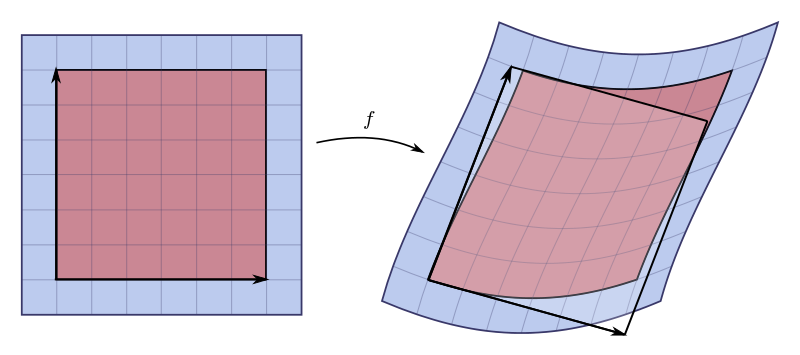
\includegraphics[width=10cm]{pics/jacobian.png}
	\end{center}

	{ \scriptsize Quelle: \url{https://en.wikipedia.org/wiki/Jacobian_matrix_and_determinant} }


	Die Jacobi-Matrix definiert eine lineare Abbildung, die $e_i \in \R^n$ auf $\pdir{f}{x_i} \in \R^m$ abbildet. Diese lineare Abbildung ist eine Approximation der Abbildung $h \mapsto f(x+h) - f(x)$ für kleine $h \in \R^n$. 
\end{bem}



\begin{bem}
	Im Spezialfall $m=1$ erhält man 
	\[
		J_f(x) := \left( \frac{\partial f}{\partial x_1} (x),\ldots, \frac{\partial f}{\partial x_n} (x) \right)
	\] als die Ableitung von $f$. 
	
	Der Vektor 
	\[
		\nabla f (x) = \begin{pmatrix} \frac{\partial f}{\partial x_1} (x) \\ \vdots \\ \frac{\partial f}{\partial x_n} (x) \end{pmatrix} 
	\] ist der \textbf{Gradient}  von $f$ (gesprochen: Nabla $f$) an der Stelle $x$. Eine weitere verbreite Bezeichnung für den Gradienten ist $\operatorname{grad} f (x)$. 
\end{bem} 


\begin{bem}
	Der Fall $m=1$ von Theorem~\ref{thm:abl:dim:n:m} kann nun so formuliert werden: 
	
	
	Ist $ f : X \to \R$ auf $X \subseteq \R^n$ differenzierbar in $x \in X$, so gilt 
	\[
		f(x+h) = f(x) + \sprod{\nabla f(x)}{h} + R(h)
	\]
	mit $\lim_{h \to 0} \frac{R(h)}{\|h\|}  = 0$. 
\end{bem} 

\begin{bsp} 
	Wir betrachten die quadratische Form $q_A(x) = \sprod{A x}{x}$ für eine symmetrische Matrix $A \in \R^{n \times n}$. Der Gradient von $q_A(x)$ kann aus der vorigen Interpretation hergeleitet werden: 
	\[
		q_A(x+h) = \sprod{A(x+h)}{x+h} = q_A(x) + 2 \sprod{A x}{h} + q_A(h)
	\]
	Hierbei ist $q_A(h)$ der Restterm mit $\lim_{h \to 0} \frac{q_A(h)}{\|h\|} = 0$. Somit ist 
	\[
		\nabla q_A (x) = 2 A x
	\]
\end{bsp} 

\begin{aufg} {\ } 
	\begin{enuma} 
		\item Zeigen Sie, dass $\nabla \|x\| = \frac{ x }{\|x\|}$ für alle $x \in \R^n \setminus \{0\}$ erfüllt ist. 
		\item Zeigen Sie, dass $\|x\|$ im Punkt $x=0$ nicht differenzierbar ist. 
		\item Sei $f$ eine Funktion auf einer Teilmenge von $\R^m$ und seien $A \in \R^{m \times n}$ und $b \in \R^m$. Berechnen Sie den Gradienten von $f( A x +b)$ in Abhängigkeit vom Gradienten von $f$. 
	\end{enuma} 
\end{aufg} 

\begin{bem}[Geometrische Bedeutung des Gradienten einer differenzierbaren Funktion] Wenn $ f: X \to \R$ mit $X \subseteq \R^n$ stetig differenzierbar ist, so gilt Folgendes: 
	\begin{enuma}
		\item Der Graph der affinen Funktion $f(a) + \sprod{\nabla f(a)}{ x-a}$ ist die Tangentialebene zum Graphen der Funktion $f$ an der Stelle $(a,f(a))$. 
		\item Der Vektor $\nabla f(a)$ ist orthogonal zur $(n-1)$-dimensionalen Niveau-Fläche
		\[
			F := \setcond{x \in X}{f(x) = f(a)}.
		\]
		an der Stelle $a$.		
		Die \textbf{Niveau-Fläche} von $f$ zum Wert $h$ ist die Menge 
		\[
			\setcond{x \in X}{f(x) = h}.
		\]
		Sie wird auch die \textbf{Niveau-Menge} und, für $n=2$, die \textbf{Niveau-Linie} genannt.
	\end{enuma} 
\end{bem} 


\begin{bem} 	
	Sei $n \ge 2$ und $X \subseteq \R^n$.
	Auch wenn $f : X \to \R$ in einem Punkt alle partiellen Ableitungen besitzt, muss $f$ in diesem Punkt nicht differenzierbar und nicht mal stetig sein. 
	Wir betrachten die folgende Funktion: 
	\[
		f(x_1,x_2) = \begin{cases} 
			0, & \text{if} \ x_1 =0 \ \text{oder} \ x_2 = 0,
			\\ 1, & \text{sonst}.
		\end{cases} 
	\]
	Es gilt offensichtlich $\frac{\partial}{\partial x_1} f (0,0) = \frac{\partial}{\partial x_2} f(0,0) = 0$, aber $f$ ist nicht stetig in $(0,0)$. 
	
	Diese Diskrepanz lässt sich folgendermaßen erklären. Die partiellen Ableitungen definiert man durch die Änderung des Eingabevektors $x = (x_1,\ldots,x_n)$ in Koordinatenrichtungen $e_1,\ldots,e_n$. Die Ableitung von $f$ an der Stelle $x$ ist dagegen  bzgl. einer beliebigen kleinen Änderung $x+h$ von $x$ definiert. 
	
\end{bem} 

\begin{defn}[Höhere partielle Ableitungen] 
	Die  \textbf{$k$-ten partiellen Ableitungen} von $f : X \to \R$ auf $X \subseteq \R^n$ sind 
	\[
		\frac{\partial^k}{\partial x_{i_1} \cdots \partial x_{i_k}} f := \frac{\partial}{\partial x_{i_1}}\frac{\partial}{\partial x_{i_2}} \cdots \frac{\partial}{\partial x_{i_k}} f.
	\]
	mit $i_1,\ldots,i_k \in \{1,\ldots,n\}$. Man nennt $f$ \textbf{$k$-mal  partiell differenzierbar bzw. stetig partiell differenzierbar}, wenn $f$ alle $k$-ten partiellen Ableitungen existieren bzw. existieren und stetige Funktionen sind. 
\end{defn} 

\begin{thm}[Schwarz]
	Sei $f :  X \to \R$ mit $X \subseteq \R^n$. 
	Wenn $f$ $k$-mal stetig partiell differenzierbar ist, dann ist die $k$-te Ableitung 
	\[
		\frac{\partial^k}{\partial x_{i_1} \cdots \partial x_{i_k}} f
	\]
	unabhängig von der Reihenfolge von $x_{i_1},\ldots, x_{i_k}$. Insbesondere gilt für $k=2$
	\[
		\frac{\partial^2}{\partial x_i \partial x_j} f = \frac{\partial^2}{\partial x_j \partial x_i} f
	\]
	für alle $i,j \in \{1,\ldots,n\}$. 
\end{thm} 

\begin{aufg}
	Vergewissern Sie sich, dass für $f(x,y) = x \sin(x^2-y^2)$ die partiellen Ableitungen 
	\begin{align*}
	\mixedpdir{f}{x}{y} & & \text{und} & & \mixedpdir{f}{y}{x}
	\end{align*}
	übereinstimmen. Berechnen Sie alle partiellen Ableitung von $f$ der Ordnung zwei. 
\end{aufg} 


\begin{thm}[Hinreichende und Notwendige Bedingung für Differenzierbarkeit] 
	Für $f : X \to \R$ mit $X \subseteq \R^n$ gelten die Implikationen:
	\begin{align*}
		\begin{array}{c}
		 \text{$f$ ist stetig partiell differenzierbar}
		\\ \Downarrow
		\\ \text{$f$ ist differenzierbar} 
		\\ \Downarrow 
		\\ \text{$f$ ist stetig und ist partiell differenzierbar}
		\end{array}
	\end{align*} 
\end{thm} 

\begin{thm} Sei $f : X \to \R$ konvexe Funktion auf $X \subseteq \R^n$ und sei $a$ innerer Punkt von $X$. Dann sind die folgenden Bedingungen äquivalent: 
	\begin{enumi}
		\item $f$ ist partiell differenzierbar in $a$. 
		\item $f$ ist differenzierbar in $a$. 
	\end{enumi} 
\end{thm} 

\begin{aufg}
	Da $f = x \sin(x^2  -y^2)$ stetig partiell differenzierbar ist, hat man für jede Wahl von $(x^\ast,y^\ast) \in \R^2$ eine Darstellung 
	\begin{align*}
		f(x,y) & =  f(x^\ast, y^\ast ) + \frac{\partial f}{\partial x} (x^\ast,y^\ast) (x-x^\ast ) + \frac{\partial f}{\partial y} (x^\ast,y^\ast) (y - y^\ast) + R(x,y)
	\end{align*}
	mit dem Restterm 
	\[
		R(x,y) : = f(x,y)  - \underbrace{\left( f(x^\ast, y^\ast ) + \frac{\partial f}{\partial x} (x^\ast,y^\ast) (x-x^\ast ) + \frac{\partial f}{\partial y} (x^\ast,y^\ast) (y - y^\ast) \right)}_{\text{lineare Approximation von $f$ am Punkt $(x^\ast,y^\ast)$}}, 
	\]
	 der die Bedingung 
	\[
			\lim_{\substack{x \to x^\ast \\ y \to y^\ast} } \frac{ R(x,y)}{\sqrt{ (x-x^\ast)^2 + (y-y^\ast)^2}} = 0
	\]
	erfüllt. Bestimmen Sie die lineare Approximation von $f$ für $x^\ast = \sqrt{\pi/2}$ und $y^\ast = \sqrt{\pi}$. 
\end{aufg} 

\section{Kettenregel}

\begin{thm}[Kettenregel]
	Für $ f : Y \to \R^k$ und $g : X \to Y$ mit $X \subseteq \R^n$ und $Y \subseteq \R^m$ gilt 
	\[
		J_{f \circ g}(x)  = J_f (g(x)) \cdot J_g (x)
	\]
	wenn $f$ und $g$ beide differenzierbar sind. 
\end{thm}

\begin{bem}[Informelle Beschreibung der Kettenregel]
	Nehmen wir an, dass wir eine Größe $f$ in Abhängigkeit von zwei Größen $u$ und $v$ dargestellt haben, wobei $u$ sowie $v$ in Abhängigkeit von $x$ und $y$ dagestellt sind. Wenn wir $u$ und $v$ als Variablen auffassen und dabei $x$ und $y$ vergessen, ist $f$ Funktion von $u$ und $v$. Wenn wir aber $u$ und $v$ als Funktionen von $x$ und $y$ interpretieren, dann ist $f$ Funktion von $x$ und $y$. Man kann also $f$ nach $u$ und $v$, als Funktion in $(u,v)$ ableiten, aber auch nach $x$ und $y$ als Funktion von $(x,y)$ ableiten. Die Ableitungen nach $(x,y)$ und nach $(u,v)$ werden durch die Kettenregel  miteinander verlinkt: 
	\begin{align*}
		\frac{\partial f}{\partial x}  & = \frac{\partial f}{\partial u} \cdot \frac{\partial u}{\partial x} + \frac{\partial f}{\partial v} \cdot \frac{\partial v}{\partial x}
		\\
	\\ \frac{\partial f}{\partial y}  & = \frac{\partial f}{\partial u} \cdot \frac{\partial u}{\partial y} + \frac{\partial f}{\partial v} \cdot \frac{\partial v}{\partial y}
	\end{align*} 
	In dieser Formel interpretiert man $f$ als Funktion von $u$ und $v$ beim Berechnen von $\frac{\partial f}{\partial u}$ und $\frac{\partial f}{\partial v}$ und als Funktion in $x$ und $y$ beim Berechnen von $\frac{\partial f}{\partial x}$ und $\frac{\partial f}{\partial y}$. Beim Berechnen der partiellen Ableitungen von $u$ und $v$ nach $x$ sowie $y$, werden $u$ und $v$ als Funktionen in $x$ und $y$ aufgefasst. 
	
	Diese zwei Gleichungen werden als Gleichungen von Funktionen in Variablen $x$ und $y$ aufgefasst. 
\end{bem} 

\begin{bem}
	Ganz analog kann man auch die Kettenregel für allgemeine multivariate Funktionen formulieren. Sei $f = f(u_1,\ldots,u_m)$ mit $u_i = u_i(x_1,\ldots,x_n)$: das heißt, $f$ hängt von $m$ Größen $u_1,\ldots,u_m$ ab, welche von $n$ Größen $x_1,\ldots,x_n$ abhängig sind. Es gilt: 
\[
\frac{\partial f}{\partial x_j} = \sum_{i=1}^m \frac{\partial f}{\partial u_i} \cdot \frac{\partial u_i}{\partial x_j}. 
\]

Diese Formel ist rein formal nicht ganz korrekt, da man $u_1,\ldots,u_m$ in einem Ausdruck als Variablen und als Funktionen in $x_1,\ldots,x_n$ auffasst. Die Formel kann man aber mit etwas Sachverstand korrekt interpretieren. So ein Gebrauch vom mathematischen Formalismus nennt man \emph{abuse of notation} im Englischen. Das ist so etwas wie sinnvoller Notationsmissbrauch: man benutzt Formalismus zwar etwas zweckentfremdet, aber in einer praktischen und berechtigten Weise.  
\end{bem} 

\begin{bsp}[Ableitungen nach den polaren Koordinaten] 
	Wir betrachten die Polarkoordinaten $ x= r \cos \phi, y = r \sin \phi$. Wie kann die Ableitung nach $\phi$ in den kartesischen Koordinaten $(x,y)$ dargestellt werden? 
	
	\begin{align*}
		 \pdir{f}{\phi} & = \pdir{f}{x} \cdot \pdir{x}{\phi} + \pdir{f}{y} \cdot \pdir{y}{\phi} = - r \sin \phi \pdir{f}{x} + r \cos \phi \pdir{f}{y} \\ & = x \pdir{f}{y} - y \pdir{f}{x}. 
	\end{align*} 
	Das zeigt 
	\[
		\pdir{f}{\phi} = x \pdir{f}{y} - y \pdir{f}{x}
	\] 
	Die Ableitung nach $\phi$ ist das Skalarprodukt des Gradienten von $f$ mit der Drehung von $(x,y)$ um den Winkel $\pi/2$. 
	
	Was ist mit der Ableitung nach $r$? 
	\begin{align*}
		\pdir{f}{r} & = \pdir{f}{x} \cdot \pdir{x}{r} + \pdir{f}{y} \cdot \pdir{y}{r} 
		\\ & = \cos \phi \pdir{f}{x} + \sin \phi \pdir{f}{y} 
		\\ & = \frac{1}{r} ( x \pdir{f}{x} + y \pdir{f}{y} )
		\\ & = \frac{1}{\sqrt{x^2 + y^2}} \left( x \pdir{f}{x} + y \pdir{f}{y} \right). 
	\end{align*}
	Der Vektor $\frac{1}{\sqrt{x^2 + y^2}} (x,y)$ hat Länge $1$ und die gleiche Richtung wie der Vektor $(x,y)$. Die Ableitung nach $r$ ist das Skalarprodukt des Gradienten mit dem Vektor $\frac{1}{\sqrt{x^2 + y^2}} (x,y)$. 
\end{bsp} 

\begin{aufg} 
	Setzen Sie das vorige Beispiele fort und bestimmen Sie Darstellungen von $\doublepdir{f}{\phi}$ und $\doublepdir{f}{r}$ in kartesischen Koordinaten $(x,y)$. 
\end{aufg} 


\begin{bem}[Zusammenhang der Richtungsableitungen des Gradienten]
	Für $f : X \to \R$ auf $X \subseteq \R^n$ gilt
	\begin{align*}
		\partial_u f(x) & = \Bigl. \pdir{}{t} f(x+ t u) \Bigr|_{t=0} 
		\\ & = \Bigl. J_f(x+ t u) \pdir{x+tu}{t} \Bigr|_{t=0}
		\\ & = \Bigl. \nabla f(x+t)^\top u \Bigr|_{t=0} 
		\\ & = \Bigl. \sprod{f(x+tu)}{u}  \Bigr|_{t=0}
		\\ & = \sprod{f(x)}{u}. 
	\end{align*}
	Fazit: 
	\[
		\partial_u f(x) = \sprod{f(x)}{u}. 
	\]
\end{bem} 

\begin{aufg}
	Benutzen Sie die Ungleichung von Cauchy-Schwarz um zu zeigen, dass die  Richtung von $\nabla f(x)$ die Richtung des größten Anstiegs von $x$ an der Stelle $f$ ist. 
\end{aufg} 


\begin{bem}[Wellengleichung in der Dimension eins]
	Seien $c>0$ die Geschwindigkeit, $t$ die Zeitvariable und $x$ die Raumvariable . Die Wellengleichung in der Dimension eins ist die Gleichung 
	\[
		 \doublepdir{u}{t} =   c^2 \doublepdir{u}{x} 
	\]
	für eine unbekannte Funktion $u(t,x)$. 
	
	Um diese Gleichung zu lösen, schreiben wir sie zuerst in einer Operator-Form um: 
	\begin{align} \label{wellen:gl:mit:op} 
		\left( c^2 \left( \pdir{}{x} \right)^2 -  \left( \pdir{}{t} \right)^2 \right) u = 0. 
	\end{align}
	Das soll heißen: Der Operator ``$c^2$ mal das zweifache Ableiten nach $x$ minus das zweifache Ableiten nach $t$'' macht aus $u$ die Nullfunktion.  Der Begriff Operator bedeutet in unseren Kontext ``eine Operation, die aus Funktionen (neue) Funktionen erzeugt''. 
		
	Nun können wir den Operator $c^2 \left( \pdir{}{x} \right)^2 -  \left( \pdir{}{t} \right)^2$ aus \eqref{wellen:gl:mit:op} mit Hilfe der dritten binomischen Formel als die Anwendung von zwei Operatoren umschreiben: 
	\[
		 c^2 \left(  \pdir{}{x} \right)^2 - \left( \pdir{}{t} \right)^2 = \left( c \pdir{}{x} -   \frac{\partial }{\partial t}   \right) \left(  c \pdir{}{x}  +  \pdir{}{t}  \right) 
	\]
	Das ergibt: 
	\begin{align} \label{wellen:zwei:op}
		\left( c \pdir{}{x} - \pdir{}{t}   \right) \left(   c \pdir{}{x} + \pdir{}{t} \right) u = 0. 
	\end{align}
	Die Bedeutung von \eqref{wellen:zwei:op} ist wie folgt: wenn wir zu $u$ den Operator $  c \pdir{}{x}  + \pdir{}{t}$ anwenden, und dann zum Ergebnis den Operator $ c \pdir{}{x}  - \pdir{}{t}$ anwenden, kriegen wir die Nullfunktion. 
	
	Es bietet sich nun die folgende Substitution an, welche die Variablen $(x,t)$ durch die Variablen $(\xi,\eta)$ ersetzt: 
	\begin{align*}
		\xi & = x -c t, 
	\\	\eta & = x + c t.
	\end{align*} 
	Denn, nach der Substitutionsregel, die wir in der Operator-Form hinschreiben, erhalten wir 
	\begin{align*}
		\pdir{}{x}  & = \pdir{\xi}{x} \cdot \pdir{}{\xi} + \pdir{\eta}{x} \cdot \pdir{}{\eta} = \pdir{}{\xi} + \pdir{}{\eta} 
		\\ 
		\\ \pdir{}{t}  & = \pdir{\xi}{t} \cdot \pdir{}{\xi} + \pdir{\eta}{t} \cdot \pdir{}{\eta} = - c \pdir{}{\xi} + c \pdir{}{\eta}
	\end{align*}
	Die beiden Operatoren aus \eqref{wellen:zwei:op} können in den neuen Variablen $(\xi,t)$ dargestellt werden: 
	\begin{align*}
		c \pdir{}{x} - \pdir{}{t} &  = c \left( \pdir{}{\xi} + \pdir{}{\eta} \right)  - \left( - c \pdir{}{\xi} + c \pdir{}{\eta} \right)  = 2 c \pdir{}{\xi}
		\\
		\\ c \pdir{}{x} + \pdir{}{t} &  = c \left( \pdir{}{\xi} + \pdir{}{\eta} \right)  + \left( - c \pdir{}{\xi} + c \pdir{}{\eta} \right)  = 2 c \pdir{}{\eta}
	\end{align*} 
	Die Gleichung \eqref{wellen:zwei:op} wird also in den neuen Variablen als 
	\[
		\pdir{}{\xi} \pdir{}{\eta} u = 0 
	\]
	dargestellt. Die vorige Gleichung bedeutet, dass $\pdir{}{\eta} u$ als Funktion von $\xi$ und $\eta$ von $\xi$ unabhängig ist: 
	\[
		\pdir{}{\eta} u = f(\eta) 
	\]
	Sei $F$ Stammfunktion von $f$. Integration der vorigen Gleichung nach $\eta$ ergibt ``$F(\xi)  + \text{Konstante}$''. Wir haben aber für jede Wahl von $\eta$ potenziell eine andere Konstante. Wir bezeichnen also die ``Konstante'' als $G(\eta)$. Wir erhalten somit die Darstellung 
	\[
		u  = F(\xi) + G(\eta) = F(x - c t) + G(x+ ct). 
	\]
	Die Funktion $u(x,t)$ setzt sich aus zwei Wellen zusammen: die Welle $F(x-ct)$, die sich mit der Geschwindigkeit $c$ nach rechts bewegt und die Welle $G(x+ct)$, die sich mit der Geschwindigkeit $c$ nach links bewegt. 
\end{bem} 

\begin{bem}[Einhüllende Kurve]
	Betrachten wir eine parametrische Schar von Kurven 
	\[
		K_s := \setcond{ (x,y) \in \R^2}{f(s,x,y) = 0},
	\]
	die implizit durch eine Gleichung $f(s,x,y) = 0$ mit einem Parameter $s \in \R$ gegeben sind. Eine \textbf{einhüllende Kurve} zu dieser Schar ist eine Kurve $K$, die in jedem Punkt durch eine der Kurven der Schar $(K_s)_{s \in \R}$ berührt wird (genaue Definition lassen wir weg). 
	
	Die Gleichung der einhüllenden Kurve kann mit Hilfe von partiellen Ableitungen bestimmt werden. Wir betrachten einen Schnittpunkt von zwei Kurven $K_s$ und $K_{s + \Delta s}$ der Schar mit $\Delta s \ne 0$. Für den Schnittpunkt $(x,y)$ gilt 
	\[
		f(s + \Delta s, x , y ) = f(s,x,y) = 0.
	\]
	Diese beiden Gleichungen kann man als 
	\begin{align*}
		f(s,x,y) & = 0,
\\
		\frac{f(s+\Delta s, x , y ) - f(s,x,y)}{\Delta s} & = 0
	\end{align*} 
	umformulieren. Wenn  wir im vorigen System für $(x,y)$ den Wert $\Delta s$ gegen $0$ schicken, so geht die Lösung $(x,y)$ dieses System gegen einen Punkt in der einhüllenden Kurve. Die Lösung erfüllt die Gleichungen 
	\begin{align*}
		f(s,x,y) & = 0 
\\		\pdir{}{s} f(s,x,y) & = 0.
	\end{align*} 
\end{bem} 

\begin{bem}[Einhüllende Wurfparabel] 
	Aus dem Punkt $x=0,y=0$ kann Objekt mit Geschwindigkeit $v$ in jede Richtung herausgeworfen werden. Welche Form hat der Bereich alle Punkte, die durch einen Wurf getroffen werden können? 
	
	Die Flugbahn in Abhängigkeit von dem Wurfwinkel $\alpha$ zur horizontalen Richtung $(1,0)$ und der Zeit $t$ ist durch die Gleichungen 
	\begin{align*}
		x & = t v \cos \alpha 
\\		y & = t v \sin \alpha  - \frac{g}{2} t^2,
	\end{align*}
	beschrieben, wobei hier $g>0$ die Fallbeschleunigung ist. Wir können $t$ eliminieren und erhalten die Formel
	\begin{align*}
		y = x \tan \alpha  - \frac{g}{2 v^2 \cos^2 \alpha} x^2,
	\end{align*} 
	die uns $y$ in Abhängigkeit von $x$ für ein gegebenes $\alpha$ beschriebt. Um Trigonometrie zu vermeiden führen wir an der Stelle von $\alpha$ 
	einen anderen Parameter  ein: $s = \tan \alpha$. So erhalten wir die parametrische Schar von Parabeln
	\begin{align*}
		y = s x - \frac{g}{2 v^2} (s^2 + 1) x^2
	\end{align*} 
	mit einem Parameter $s \in \R$. 
	Der Bereich, der durch die Parabeln unserer Schar abgedeckt ist, ist durch die einhüllende Kurve dieser Schar beschränkt. Das Eliminieren von $s$ im System
	\begin{align*}
		y & = s x - \frac{g}{2 v^2} (s^2 + 1) x^2
\\		\pdir{}{s} y & = \pdir{}{s} \left( s x - \frac{g}{2 v^2} (s^2 + 1) x^2 \right)
	\end{align*} 
	gibt uns die Gleichung 	
	\[
		y = \frac{v^2}{2 g} - \frac{g}{2 v^2} x^2
	\]
	für die einhüllende Kurve. 
	
	\begin{center}
	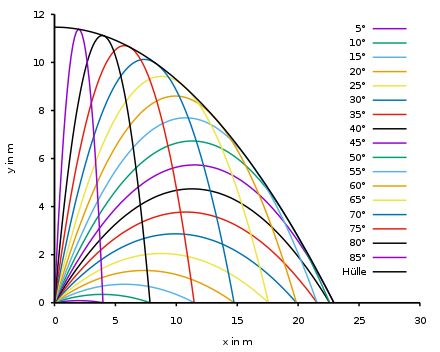
\includegraphics[width=20em]{pics/wurf.png}	
	\end{center}

	{\scriptsize Quelle: \url{https://de.wikipedia.org/wiki/Wurfparabel} } 
\end{bem} 

\begin{aufg}
	Bestimmen Sie die einhüllende der Wurfparabeln elementar mit der Verwendung der $pq$-Formel. % Butikov et al., Teil I, \S~13. Grenze der erreichbaren Ziele. 
\end{aufg} 

\section{Totales Differential und implizite Funktionen} 

\begin{bem} 
	Beispiel im Fall von zwei Variablen. Das \textbf{totale Differential} von $F = F(x,y)$ ist der Ausdruck 
	\[
		\dd F = \pdir{F}{x} \dd x + \pdir{F} x \dd y. 
	\]
	Definition im Fall von mehr als zwei Variablen analog. Für jede Wahl von $(x,y)$ ist $\dd F$ eine lineare Funktion in $(\dd x, \dd y)$. Bedeutung 
	\[
		\Delta F \approx \pdir{F}{x} \Delta x + \pdir{F}{x} \Delta y. 
	\]
	Zweite Bedeutung, das Ableitung nach einer Anonymen Variablen. Wenn wir für $x$ und $y$ Funktionen $x=x(t)$ und $y=y(t)$ in $t$ einsetzen, ist $F(x(t),y(t))$ ebenfalls Funktion in $t$. Nach der Kettenregel gilt: 
	\begin{align*}
		\frac{ \dd F }{\dd t} = \pdir{F}{x} \cdot \frac{\dd x}{\dd t} + \pdir{F}{y} \cdot \frac{\dd y}{\dd t}. 
	\end{align*} 
	Im Ausdruck für das totale Differential wird ``das Teilen durch $\dd t$ weggekürzt'' (das eine informelle Beschreibung). 
\end{bem} 

\begin{bem}
	Angenommen wir haben eine Gleichung $F(x,y) = 0$, die uns $y$ als Funktion von $y$ Beschreibt. Man sagt in diesem Fall, dass $y$ eine implizite Funktion ist (oder, $y$ von $x$ ist als eine implizite Funktion definiert). Aus dieser Gleichung kann man mit der Verwendung des totalen Differential die Ableitung von $y$ nach $x$ ausrechnen. Aus $F(x,y) = 0$ erhalten wir 
	\[
		0 = \dd F = \pdir{F}{x} \dd x + \pdir{F}{y} \dd y
	\]
	Wenn $\pdir{F}{y} \ne 0$ ist, erhalten wir also 
	\[
		\frac{\dd y}{\dd x} =  - \frac{\pdir{}{x} F}{\pdir{}{y} F}.
	\]
	Diese rein formale Berechnung hat eine korrekte Interpretation als die Awendung der Kettenregel zur Gleichung $F(x,y(x) ) = 0$ für eine Funktion $y(x)$. 
\end{bem} 

\section{Extremwertaufgaben}

\begin{defn}
	\textbf{Lokale/globale Minima/Maxima/Extrema} einer multivariaten Funktion werden genauso wie  im univariaten Fall definiert. 
\end{defn}

\begin{thm}
 	Sei $f : X \to \R$ konvexe Funktion auf $X \subseteq \R^n$ und sei $a \in X$. Dann sind die folgenden Bedingungen äquivalent: 
 	\begin{enumi}
 		\item $f$ erreicht in $a$ ein lokales Minimum. 
 		\item $f$ erreicht in $a$ ein globales Minimum. 
 	\end{enumi} 
\end{thm} 


\begin{thm}[Notwendige Bedingung] 
	Sei $f : X \to \R$ partiell differenzierbar und sei $a \in X$ innerer Punkt von $X \subseteq \R^n$. Erreicht $f$ in $a$ ein lokales Extremum, so gilt $\nabla f(a) =0$. 
\end{thm} 

\begin{defn} 
	Für $f : X \to \R$ nennen wir einen Punkt $a \in X$ von $f$ kritisch bzw. stationär, wenn $f$ in $a$ differenzierbar ist und der Gradient von $f$ an der Stelle $a$ gleich $0$ ist. 
\end{defn} 

\begin{bsp}
	Wir bestimmen das Minimum 
	$f(x,y) = 2 y^2  + (x^2-2) x^2 + 2 x^2 y$ über $\R^2$. Die Funktion ist überall differenzierbar und auf dem gesamten $\R^2$ definiert. Darüber hinaus gilt $f \to \infty$ für $x^2 + y^2 \to \infty$, sodass die Funktion ihr Minimum erreicht.  Es reicht also aus, alle stationären Punkte auszurechnen, und die Werte der Funktion an den stationären Punkten gegeneinander zu vergleichen. 
	
	Man hat
	\begin{align*}
		\pdir{f}{x} & = 4 x^3 - 4 x + 4 x y
		\\ \pdir{f}{y} & = 2 y + 2 x^2
	\end{align*} 
	
	Wir lösen das System 
	\begin{align*} 
		4 x^3 - 4 x + 4 x y& = 0,
		\\ 4 y + 2 x^2 & = 0
	\end{align*} 
	um die stationären Punkte auszurechnen. 
	
	Dabei unterscheiden wir zwischen $x = 0$ und $x \ne 0$. Bei $x=0$ ist $x=0,y=0$ die einzige Lösung. Bei $x \ne 0$ können wir die erste Gleichung durch $ x$ teilen. Das ergibt (durch das zusätzliche Teilen durch Konstante) das System. 
	\begin{align*}
		x^2 - 1 +  y & = 0 
	\\	2 y + x^2 & =0. 
	\end{align*} 
	Das vorige System ist linear in $x^2$ und $y$. Wir erhalten $x^2 = 2, y = -1$. 
	
	Insgesamt erhalten wir also die drei stationären Punkte: $(0,0), (- \sqrt{2},0), (\sqrt{2},0)$. 
	
	Die Werte der Funktion $f$ an diesen Punkten sind: 
	\begin{align*}
		f(0,0) & = 0
		\\ f(\sqrt{2},-1) & =  -2,
		\\ f(-\sqrt{2},-1) & = -2.
	\end{align*} 
	Das Minimum wird somit an zwei Stellen $(\sqrt{2}, -1)$ und $(-\sqrt{2},-1)$ erreicht. 
\end{bsp} 


\begin{thm} 
	Sei $f : X \to \R$ konvexe Funktion auf $X \subseteq \R^n$ und sei $a$ innerer Punkt von $X$, in dem die Funktion $f$ differenzierbar ist. Dann sind die folgenden Bedingungen äquivalent: 
	\begin{enuma}
		\item $f$ erreicht in $a$ ein lokales Minimum. 
		\item $f$ erreicht in $a$ ein globales Minimum. 
		\item $\nabla f(a) = 0$. 
	\end{enuma} 
\end{thm} 



\begin{aufg}
	Seien $a, b, c \in \R^2$ Ecken eines Dreiecks. Wir minimieren $f(x) = \|x - a\| +\|x-b\| + \|x - c\|$ über $\R^2$. Da die Funktion $f$ stetig ist und man $f(x) \to \infty$ für $\|x\| \to \infty$ hat, wird das Minimum erreicht. Welche Punkte von $\R^2$ kommen als optimale Lösungen in Frage? Beschreiben Sie die Punkte geometrisch.
	Man beachte, dass $f(x)$ nicht überall differenzierbar ist. 
\end{aufg} 

\begin{aufg}
	Nehmen wir an, dass ein Roboter in der Lage ist, sich in der oberen Halbebene 
	\[
		H^+ = \setcond{(x_1,x_2) \in \R^2}{x_2 \ge 0}
	\] mit einer Geschwindigkeit $v>0$ Einheiten pro Sekunde zu bewegen, und in der unteren Halbebene 
	\[
		H^- = \setcond{(x_1,x_2) \in \R^2}{x_2 \le 0}
	\] mit der Geschwindigkeit $w>0$ Einheiten pro Sekunde. Der Roboter soll von einem Punkt $a \in H^+$ in der oberen Halbebene einen Punkt $b \in H^-$ in der unteren Halbebene schnellstmöglich erreichen. In welchem Punkt $(s,0)$ mit $s \in \R$ soll der Übergang von der oberen in die untere Halbebene stattfinden? Der Roboter bewegt sich geradlinig von $a$ zu $(s,0)$ mit Geschwindigkeit $v$ und anschließend von $(s,0)$ zu $b$ geradlinig mit Geschwindigkeit $w$. Beschreiben Sie die Optimale Wahl des Übergangpunkts $(s,0)$ geometrisch. 
\end{aufg} 

\section{Multidimensionale Taylorentwicklung} 

\begin{bem}
	Zuerst formulieren wir die Entwicklung mit Hilfe des Operators für die Berechnung der Richtungsableitung:
	\[
		\partial_h := h_1 \pdir{}{x_1} +  \cdots + h_n \pdir{}{x_n}. 
	\]
\end{bem} 

\begin{thm}[Multidimensionale Taylorentwicklung, Hilfsformulierung]
	\label{thm:multdim:taylor:hilf}
	Sei $ f : X \to \R^n$ eine $(N+1)$-mal stetig differenzierbare Funktion auf einer offenen konvexen Teilmenge $X \subseteq \R^n$ und sei $x \in X$. Dann gilt 
	\begin{equation}
		\label{eq:multidim:taylor:formel:hiilfs}
		f(x+h) = 	\sum_{k=0}^N \frac{1}{k!} \left(h_1 \pdir{}{x_1} +  \cdots + h_n \pdir{}{x_n} \right)^k f (x) + O(\|h\|^{N+1}),
	\end{equation}
	für $h = (h_1,\ldots,h_n) \to 0$.
\end{thm} 

\begin{bem}
	Theorem~\ref{thm:multdim:taylor:hilf} folgt aus dem univariaten Fall der Taylorentwicklung. Man beachte, dass die Ableitungen $(\partial_u)^k f(x)$ mit $0 \le k \le N$, die man in dieser Entwicklung benutzt Ableitungen der Ordnung bis zu $N$ für die selbe Richtung $u$ sind. Das erstellt den Bezug zur Dimension eins. Nun wollen wir aber Formel \eqref{eq:multidim:taylor:formel:hiilfs} in eine explizite Form mit partiellen Ableitung der Ordnung höchstens $N$ überführen, indem wir den Operator-Ausdruck
	\[
		\left(h_1 \pdir{}{x_1} +  \cdots + h_n \pdir{}{x_n} \right)^k
	\]
	ausmultiplizieren. Dafür benötigen wir die Multinomialformel

\end{bem} 

\begin{bem}[Multinomialformel]
	\[
		(u_1 + \cdots + u_n)^k =  \sum_{\substack{p_1,\ldots,p_n \ge 0 \ : \\p_1 + \cdots + p_n = k}} \frac{k!}{p_1! \cdots p_n !} u_1^{p_1} \cdots u_n^{p_n}.
	\]

	Hierbei ist $\frac{k!}{p_1! \cdots p_n !}$ der sogenannte \textbf{Mutlinomialkoeffizient}; Bezeichnung dafür: 
	\[
		\binom{k}{p_1 ,\cdots, p_n}. 
	\]
	
	Der \textbf{binomische Lehrsatz} ist der Fall $n=2$ der Multinomialformel. 
\end{bem} 

\begin{bem}[Kombinatorische Bedeutung der multinomialen Koeffizienten]
	{\ } 
	
	Die Multinomiale Koeffizienten haben eine kombinatorische Bedeutung. Dementsprechend hat die Multinomialformel eine kombinatorische Begründung. 
	
	Hier ein Beispiel zur kombinatorischen Bedeutung der Multinomialkoeffizienten: Für jedes der $10$ gegebenen Fächer bekommt eine Abschlussnote. Die Anzahl der Möglichkeiten, $4$ Einsen, $3$ Zweien und $2$ Dreien zu bekommen ist 
	\[
		\frac{10!}{ 4! \cdot 3! \cdot 2!} 
	\]
\end{bem} 

\begin{bem}[Ein Analogon des pascalschen Dreiecks.]
		\begin{center}
		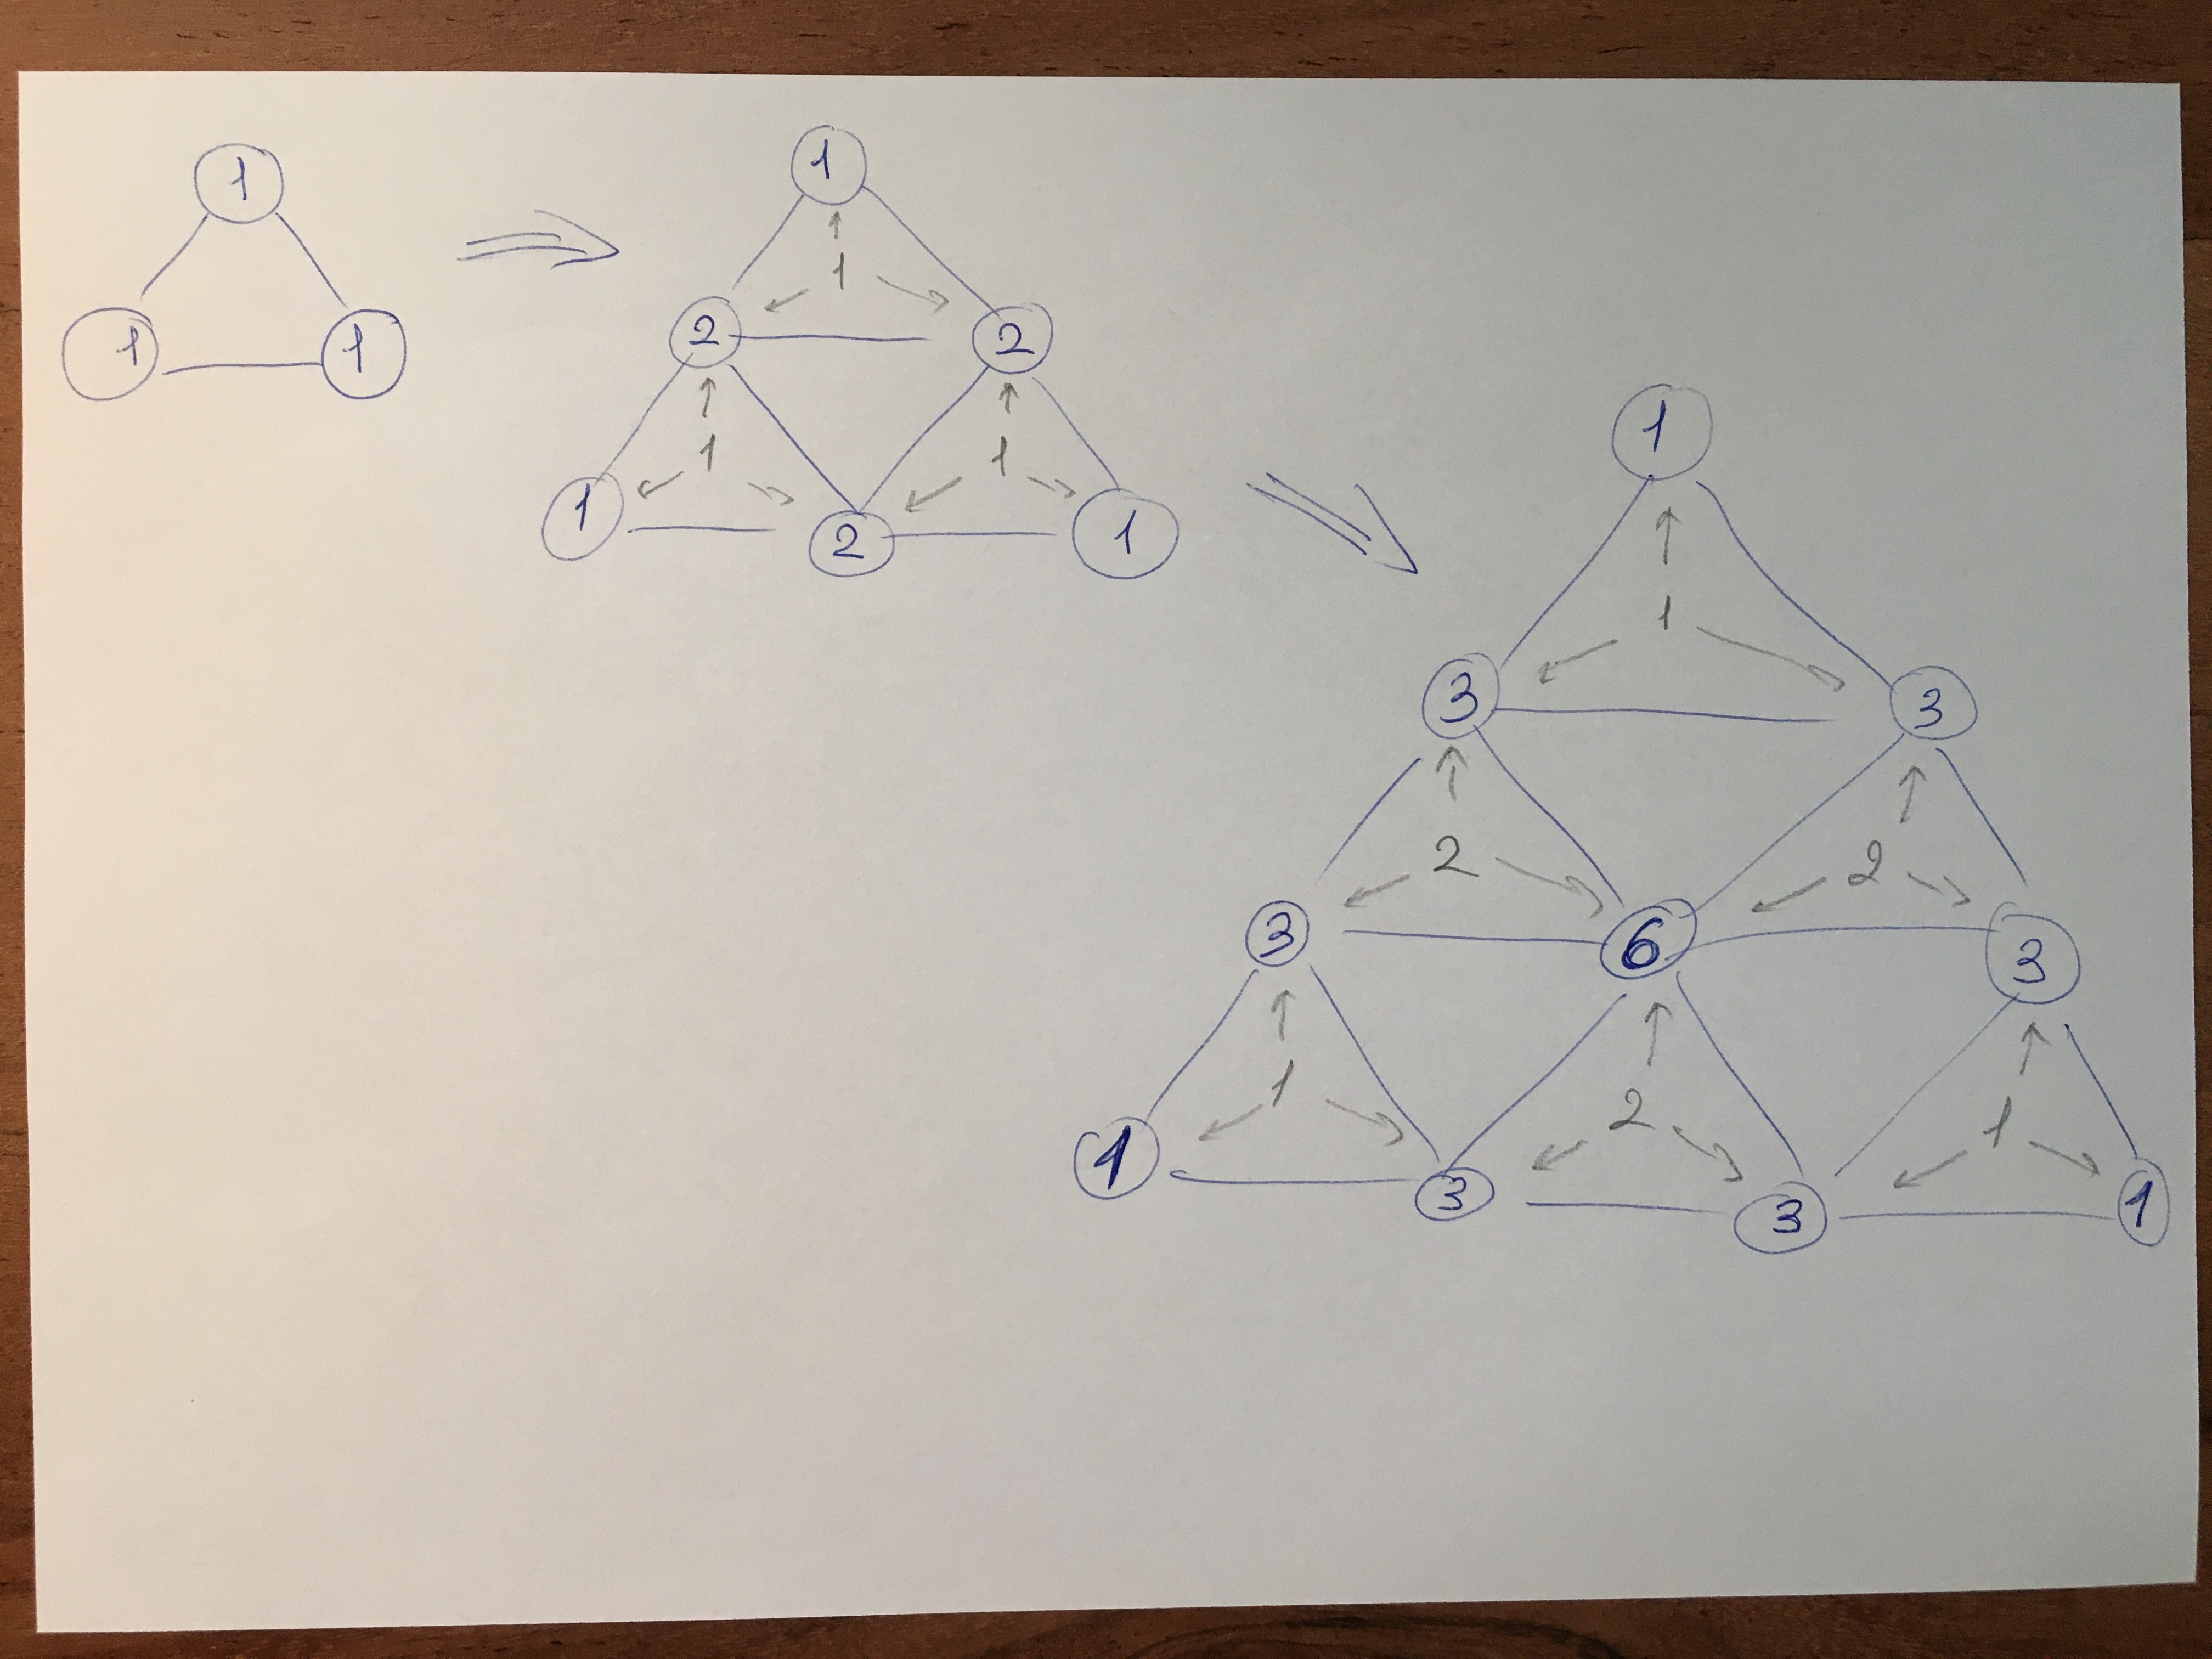
\includegraphics[width=0.8\textwidth]{pics/mega_pascal.jpg}
	\end{center}
\end{bem} 


\begin{bem}[Multidimensionale Taylorentwicklung, Formulierung~A]
	\[
		f(x+ h) =  \sum_{\substack{p_1,\ldots,p_n \ge 0 \ : \\p_1 + \cdots + p_n \le N}} \frac{1}{p_1! \cdots p_n !} \cdot \frac{\partial^{p_1+ \cdots +p_n} f}{\partial x_1^{p_1} \cdots \partial x_n^{p_n}} (x) h_1^{p_1} \cdots h_n^{p_n} + O(\|h\|^{N+1})
	\]
	für $h= (h_1,\ldots,h_n) \to 0$. 
\end{bem}

\begin{bem}[Multidimensionale Taylorentwicklung, Formulierung~B]
		\[
	f(x) = \sum_{\substack{p_1,\ldots,p_n \ge 0 \ :\\p_1 + \cdots + p_n \le N}} \frac{1}{p_1! \cdots p_n !} \cdot \frac{\partial^{p_1 + \cdots + p_n} f}{\partial x_1^{p_1} \cdots \partial x_n^{p_n}} (a) (x_1-a_1)^{p_1} \cdots (x_n - a_n)^{p_n} + O(\|x-a\|^{N+1})
	\]
	für $x = (x_1,\ldots,x_n) \to a = (a_1,\ldots,a_n)$.
\end{bem} 

\begin{defn}
	Das $n$-variate Polynom 
	\[
	T_N(x) := \sum_{\substack{p_1,\ldots,p_n \ge 0 \ :\\p_1 + \cdots + p_n \le N}} \frac{1}{p_1! \cdots p_n !} \cdot \frac{\partial^{p_1 + \cdots + p_n} f}{\partial x_1^{p_1} \cdots \partial x_n^{p_n}} (a) (x_1-a_1)^{p_1} \cdots (x_n - a_n)^{p_n}
	\]
	nennt man das \textbf{Taylorpolynom} der Ordnung $N$ zum Entwicklungspunkt $a$ für die Funktion $f$. 
\end{defn} 

\begin{bem}[Spezialfall: Ordnung~1] 
	\[
		f(x+ h) =f(x)+ \sprod{\nabla f (x)}{h} + O(\|h\|^2)
	\]
	für $h \to 0$. 
	
	Lokale Approximation durch Polynom vom Grad $1$. Relevant für notwendige Bedingung $\nabla f(x) =0$ der lokalen Optimalität. 
\end{bem}

\begin{bem}[Spezialfall: Ordnung~2]
	\[
		f(x+h) = f(x) + \sprod{\nabla f (x)}{h} + \frac{1}{2} \sum_{i,j=1,\ldots,n} \mixedpdir{}{x_i}{x_j} f (x) h_i h_j + O(\|h\|^3)
	\]	
	für $h = (h_1,\ldots,h_n) \to 0$. 
	
	Lokale Approximation durch Polynom vom Grad $2$. Relevant für notwendige und hinreichende Bedingungen der Optimalität (die wir im Folgenden diskutieren). 
\end{bem}  

\section{Extremwertaufgaben: Bedingungen zweiter Ordnung} 


\begin{defn}
	Die \textbf{Hesse-Matrix} von $f : X \to \R$ mit $X \subseteq \R^n$ ist die $n \times n$ Matrix der zweiten partiellen Ableitungen
	\[
		\nabla^2 f := \biggl( \frac{\partial^2 f}{\partial x_i \partial x_j}  \biggr)_{i,j=1,\ldots,n}
	\]
	Weitere Bezeichnung: $H_f(x)$. 
\end{defn} 

\begin{bem}[Spezialfall: Taylorentwicklung der Ordnung~2 mit Hesse-Matrix]
	\begin{align*}
	f(x+h) & = f(x) + \sprod{\nabla f (x)}{h} + \frac{1}{2} \sprod{h}{\nabla^2 f(x) h} + O(\|h\|^3)
	\end{align*}
	oder mit etwas anderen Bezeichnungen
	\begin{align*} 
	f(x+h) & = f(x) + \nabla f(x)^\top h + \frac{1}{2} h^\top \nabla^2f(x) h + O(\|h\|^3)
	\end{align*}
\end{bem} 

\begin{thm}[Notwendige Bedingungen zweiter Ordnung] 
	Sei $f : X \to \R$ $2$-mal stetig partiell differenzierbar und sei $a \in X$ innerer Punkt von $X$. Dann gilt: 
	\begin{enuma}
		\item Erreicht $f$ in $a$ ein lokales Minimum, so ist $\nabla f(a) =0$ und $\nabla^2 f(a)$ positiv \underline{semi}definit.
		\item Erreicht $f$ in $a$ ein lokales Maximum, so ist $\nabla f(a) =0$ und $\nabla^2 f(a)$ negativ \underline{semi}definit.
	\end{enuma}
\end{thm} 

\begin{thm}[Hinreichende Bedingungen zweiter Ordnung]
	Sei $f : X \to \R$ $2$-mal stetig partiell differenzierbar und sei $a \in X$ innerer Punkt von $X$. Dann gilt: 
\begin{enuma}
	\item Ist $\nabla f(a) =0$ und $\nabla^2 f(a)$ positiv definit, dann erreicht $f$ in $a$ ein lokales Minimum.
	\item Ist $\nabla f(a) =0$ und $\nabla^2 f(a)$ negativ definit, dann erreicht $f$ in $a$ ein lokales Maximum.
\end{enuma}
\end{thm} 

\section{Wiederholung: semidefinite und definite symmetrische Matrizen} 

\begin{defn}
	Eine Matrix $A = (a_{ij})_{i,j} \in \R^{n \times n}$ heißt symmetrisch, wenn $a_{ij} = a_{ji}$ für alle $i,j \in \{1,\ldots,n\}$ gilt. Mit Transposition schreibt man diese Bedingung als $A =A^\top$. 
	
	Die Funktion $q_A(x) := x^\top A x$ heißt \textbf{quadratische Form}. 
	zur symmetrischen Matrix  $A = (a_{ij})_{i,j} \in \R^{n \times n}$. Mit Koordinaten:
	\[
		q_A(x_1,\ldots,x_n) = \sum_{i,j =1,\ldots,n} a_{ij} x_i x_j.
	\]
\end{defn} 


\begin{defn} 
		Symmetrische Matrix $A \in \R^{n \times n}$ bzw. die quadratische Form $q_A(x)$ heißt: 
	\begin{itemize}
		\item \textbf{positiv semidefinit}, wenn $q_A(x) \ge 0$ für alle $x \in \R^n$ gilt, 
		\item \textbf{positiv definit}, wenn $q_A(x)>0$ für alle $x \in \R^n \setminus \{0\}$ gilt, 
		\item \textbf{negativ semidefinit}, wenn $q_A(x) \le 0$ für alle $x \in \R^n$ gilt, 
		\item \textbf{negativ definit}, wenn $q_A(x) < 0$ für alle $x \in \R^n \setminus \{0\}$ gilt. 
		\item \textbf{indefinit}, wenn es $x \in \R^n$ mit $q_A(x)<0$ sowie  $x \in \R^n$ mit $q_A(x) >0$ existieren. 
	\end{itemize} 
\end{defn} 

\begin{thm}
 	Sei $A \in \R^{n \times n}$ symmetrisch. Dann sind alle Eigenwerte von $A$ reell. Darüber hinaus besitzt $\R^n$ eine Orthogonalbasis aus Eigenvektoren von $A$. 
\end{thm} 

\begin{bem}
	Die Eigenwerte sind Nullstellen des characteristischen Polynoms $\det(\lambda I - A)$. Im Allgemeinen sind es komplexe Zahlen, das vorige Theorem garantiert aber, dass für symmetrische Matrizen $A$, die Eigenwerte stets reell sind.
\end{bem} 


\begin{thm}
	Sei $A \in \R^{n \times n}$ symmetrisch. Dann gilt: 
	\begin{enuma}
		\item $A$ positiv semidefinit $\Leftrightarrow$ alle Eigenwerte von $A$ sind $\ge 0$. 
		\item $A$ positiv definit $\Leftrightarrow$ alle Eigenwerte von $A$ sind $>0$. 
		\item $A$ negativ semidefinit $\Leftrightarrow$ alle Eigenwerte von $A$ sind $\le 0$. 
		\item $A$ negativ definit $\Leftrightarrow$ alle Eigenwerte von $A$ sind $<0$. 
		\item $A$ indefinit $\Leftrightarrow$ $A$ besitzt positive sowie negative Eigenwerte. 
	\end{enuma} 
\end{thm} 

\begin{bsp}
	\[
		A = \begin{pmatrix} 1 & -3 \\ -3  & 9 \end{pmatrix}.
	\]
	Wir lösen die charakteristische Gleichung 
	\[
		\begin{vmatrix} 1 - \lambda & -3 \\ -3 & 9 - \lambda \end{vmatrix} =0
	\]
	und erhalten $0$ und $10$ als Lösungen. Somit ist $A$ positiv semidefinit (aber nicht positiv definit, wegen der $0$). 
\end{bsp} 

\begin{bsp}
	\[
		A = \begin{pmatrix} -4 & 10 \\ 10  & -25 \end{pmatrix}
	\]
	Wir lösen die charakteristische Gleichung 
	\[
	\begin{vmatrix} -4 - \lambda & 10 \\ 10 & -25 - \lambda \end{vmatrix} =0
	\]
	und erhalten $0$ und $-29$ als Lösungen. Somit ist $A$ negativ semidefinit (aber nicht negativ definit, wegen der $0$). 
\end{bsp} 

\begin{bsp}
	\[
		A = \begin{pmatrix} 5 & -1 \\ -1 & 2 \end{pmatrix}. 
	\]
	Wir lösen die charakteristische Gleichung 
	\[
		\begin{vmatrix} 5 - \lambda & - 1 \\ -1 & 2 - \lambda \end{vmatrix} = 0 
	\]
	und erhalten $3 \frac{1}{2} \pm \sqrt{ ( 3 \frac{1}{2})^2 - 9 }$ als Lösungen. Da die beiden Lösungen positiv sind, ist die Matrix $A$ positiv definit. 
\end{bsp} 

\begin{bem}
	Es gibt ein Resultat, das uns ermöglicht, die Berechnung der Eigenwerte zu vermeiden...
\end{bem}

\begin{thm} 
	Sei $A \in \R^{n \times n}$ symmetrisch. Dann gilt: 
	\begin{enuma}
	\item $A$ positiv semidefinit $\Leftrightarrow$ die Koeffizienten $c_1,\ldots,c_n$ vom Polynom  
	\[
		\det(\lambda I + A) = \lambda^n + c_1 \lambda^{n-1} + \cdots + c_n \lambda^0
	\] sind alle $\ge 0$.  
	\item $A$ positiv definit $\Leftrightarrow$ die Koeffizienten $c_1,\ldots,c_n$ vom Polynom  
	\[
	\det(\lambda I + A) = \lambda^n + c_1 \lambda^{n-1} + \cdots + c_n \lambda^0
	\] sind alle $> 0$.  
	\item $A$ negativ semidefinit $\Leftrightarrow$ die Koeffizienten $d_1,\ldots,d_n$ vom Polynom  
\[
\det(\lambda I - A) = \lambda^n + d_1 \lambda^{n-1} + \cdots + d_n \lambda^0
\] sind alle $\ge 0$.  
\item $A$ negativ definit $\Leftrightarrow$ die Koeffizienten $d_1,\ldots,d_n$ vom Polynom  
\[
\det(\lambda I - A) = \lambda^n + d_1 \lambda^{n-1} + \cdots + d_n \lambda^0
\] sind alle $> 0$.  
\end{enuma} 
\end{thm} 

\begin{bem}
	$f_A(\lambda) := \det(\lambda I - A)$ ist das charakteristische Polynom und $\det(\lambda I + A)$ ergibt sich aus dem charakteristischen Polynom: 
	\[
		\det(\lambda I + A) = (-1)^n f_A( - \lambda)
	\]
	für $A \in \R^{n \times n}$. Das bedeutet, dass man die Art von $A$ (positiv/negativ definit bzw. semidefinit or indefinit) anhand der Vorzeichen der  Koeffizienten des charakteristischen Polynoms $f_A(\lambda)$ entscheiden kann. 
\end{bem} 

\begin{bem} 
	Für eine Matrix 
	\[
		A = \begin{pmatrix} a_{11} & a_{12} \\ a_{21} & a_{22} \end{pmatrix} \in \R^{2 \times 2}.
	\]
	ist 
	\[
		\det(\lambda I - A) = \lambda^2 - \tr(A) \lambda + \det(A)
	\]
	Das führt zum folgenden Resultat: 
	\begin{align*}
		\tr(A) & = a_{11} + a_{22}  & & \text{(Spur)},
	\\	\det(A) & = a_{11} a_{22} - a_{12} a_{21} & & \text{(Determinante)}.
	\end{align*}
\end{bem} 

\begin{thm}
		Sei $A \in \R^{2 \times 2}$ symmetrisch. Dann gilt:
	\begin{enuma} 
		\item $A$ positiv semidefinit $\Leftrightarrow$ $\tr(A) \ge 0, \det(A) \ge 0$. 
		\item $A$ positiv definit $\Leftrightarrow$ $\tr(A) > 0, \det(A) > 0$. 
		\item $A$ negativ semidefinit $\Leftrightarrow$ $\tr(A) \le 0, \det(A) \ge 0$. 
		\item $A$ negativ definit $\Leftrightarrow$ $\tr(A) < 0, \det(A) > 0$. 
		\item $A$ indefinit $\Leftrightarrow$ $\det(A) < 0$
	\end{enuma} 
\end{thm} 

\begin{aufg}
	Kann eine symmetrische Matrix $A \in \R^{3 \times 3}$ mit $\det(A) < 0$:
	\begin{enuma} 
		\item positiv semidefinit sein? 
		\item positiv definit sein? 
		\item negativ semidefinit sein? 
		\item negativ definit sein? 
		\item indefinit sein? 
	\end{enuma} 
	Beantworten Sie die selben Fragen für 
	\begin{itemize}
		\item eine symmetrische Matrix $A \in \R^{4 \times 4}$ mit $\det(A) < 0$. 
		\item eine symmetrische Matrix $A \in \R^{4 \times 4}$ mit $\tr(A) >0$ ($\tr(A)$ ist die Summe der Diagonalemente von $A$). 
	\end{itemize} 
\end{aufg} 


\begin{bem}
	Eine andere Weise, die Art einer symmetrischen Matrix $A \in \R^{n \times n}$ zu Bestimmen ist durch Diagonalisierung er quadratischen Form $q_A(x)$. Man kann eine reguläre Matrix $U$ bestimmen (ein anderes Koordinatensystem) für welche die quadratische Form $q_A(U x)$ diagonal ist, das heißt 
	\[
		q_A(U x) = \gamma_1 x_1^2 +  \cdots + \gamma_n x_n^2
	\] 
	gilt für gewisse $\gamma_1,\ldots,\gamma_n \in \R$. Das Diagonalisierungsverfahren sieht dem Gauß-Verfahren sehr ähnlich. TO DO: Mehr Details. 
\end{bem} 


\section{Restringierte Optimierungsaufgaben} 

TODO: KKT für eine Gleichheitsbedingung. KKT für mehrere Gleichheitsbedingungen. 

\chapter{Integralrechnung II}


\section{Riemann-Integral} 

\begin{defn}
	Ein $n$-dimensionaler (achsenparalleler) \textbf{Quader}  $Q \subseteq \R^n$ ist kartesisches Produkt 
	\[
		Q := [a_1,b_1] \times \cdots \times [a_n,b_n]
	\] 
	von $n$ abgeschlossenen Intervallen $[a_i,b_i]$ mit $a_i < b_i$ für $i \in \{1,\ldots,n\}$. Für $n=1$ist $Q$ ein abgeschlossenes Intervall, für $n=2$ ein achsenparalleles Rechteck, und für $n=3$ ein $3$-dimensionaler Quader. Das \textbf{Volumen} von $Q$, wird als 
	\[
		\vol(Q) = (b_1-a_1) \cdot \ldots \cdot (b_n - a_n)
	\]
	definiert. 
\end{defn} 

\begin{bem}
	Der Durchschnitt von zwei Quadern 
	\[
		Q = I_1 \times \cdots \times I_n
	\]
	und 
	\[
		R = J_1  \times \cdots \times J_n
	\]
	ist gleich 
	\[
		Q \cap R = (I_1 \cap J_1) \times \cdots \times (I_n \cap J_n). 
	\]
	Dieser Durchschnitt ist nur dann wieder ein Quader, wenn alle Durchschnitte $I_k \cap J_k$ mit $k \in \{1,\ldots,n\}$ nichtentartete Segmente sind.
\end{bem} 

\begin{defn}
	Wir sagen, dass sich zwei $n$-dimensionale Quader $Q$ und $R$ \textbf{überlappen}, wenn ihr Durchschnitt $Q \cap R$ wieder ein $n$-dimensionaler Quader ist. 
\end{defn} 

\begin{defn} 
	Eine \textbf{Zerlegung} $Z$ eines $n$-dimensionalen Quaders $Q$ ist eine Menge $Z = \{Q_1,\ldots,Q_m\}$ von endlich vielen Quadern, die sich paarweise nicht überlappen, und deren Vereinigung $Q_1 \cup \cdots \cup Q_m$ mit $Q$ übereinstimmt. Diese Definition erweitert den Begriff der Zerlegung von der Dimension $n=1$ auf den Fall einer allgemeinen Dimension $n \in \N$. 
\end{defn} 

\begin{defn} 
	Für eine Funktion $f : Q \to \R$ auf einem Quader $n$ und eine Zerlegung $Z= \{Q_1,\ldots,Q_m\}$ von $Q$, definiert man die \textbf{Ober-} bzw. die \textbf{Untersumme} von $f$ bzgl. $Z$ als 
	\begin{align*}
		O_f(Z) & := \sum_{i=1}^m \sup_{x \in Q_i} f(x) \vol(Q_i), 
\\		U_f(Z) & := \sum_{i=1}^m \inf_{x \in Q_i} f(x) \vol(Q_i).
	\end{align*} 
	Des weiteren definiert man das \text{Ober-} bzw. das \textbf{Unterintegral} von $f$ auf $Q$ als 
	\begin{align*}
		O_f & := \inf_{Z \ \text{Zerlegung von} \  Q} O_f(Z),
		\\ U_f & := \sup_{Z \ \text{Zerlegung von} \ Q}	U_f(Z)
	\end{align*}
	Mann nennt die Funktion $f$ \textbf{Riemann-integrierbar} über $Q$, wenn $O_f=U_f$ gilt. In diesem nennt man den Wert $O_f = U_f$ das Riemann integral von $f$ über $Q$. Bezeichnung: 
	\begin{align*}
		\int_Q f(x) \dd x. 
	\end{align*} 
	Bei $x = (x_1,\ldots,x_n)$ schreibt man $\dd x$ in Koordinaten als $\dd x_1 \cdots \cdot \dd x_n$.  
\end{defn} 

\begin{defn} 
	Ist $ f: D \to \R$ auf einem beliebigen beschränkten Bereich $D \subseteq \R^n$ definiert, führt man das \textbf{Riemann-Integral} als 
	\[
		\int_D f (x) \dd x := \int_Q g(x) \dd x, 
	\]
	für einen Quader $Q$ mit $D \subseteq Q$ und die Funktion 
	\[
		g(x) := \begin{cases} f(x) & \text{für} \ x \in D,
			\\ 0 & \text{sonst}. 
		\end{cases}
	\]
	Die Funktion $f$ nennt man \textbf{Riemann-integrierbar} über $D$, wenn das Integral $\int_Q g(x) \dd x$ oben existiert (in diesem Fall hängt der Wert $\int_Q g(x) \dd x$ von der konkreten Wahl $Q$ des Umgebungsquader nicht ab). 
\end{defn} 

\begin{defn}
	Wenn für eine beschränkte Menge $D \subseteq \R^n$, die Konstante $1$ über $D$ \textbf{Riemann-Integrierbar} ist, dann nenn wir
	\[
		\vol(D) := \int_D 1 \dd x
	\]
	das Volumen von $D$. 
\end{defn} 

\begin{thm}
	Wenn eine Funktion $f : A\cup B \to \R$ über $A \subseteq \R^n$ und $B \subseteq \R^n$ Riemann-integrierbar ist, und $A\cap B$ keine innere Punkte hat, dann gilt 
	\[
		\int_{A \cup B}  f(x) \dd x = \int_A f(x) \dd x  + \int_B f(x) \dd x.
	\]
\end{thm} 

\begin{thm}
	Sind $f, g: D \to \R$ beide Riemann-integrierbar über $D \subseteq \R^n$, dann ist $\alpha f + \beta g$ für jede Wahl von $\alpha, \beta \in \R$ ebenfalls Riemmann-integrierbar über $D$, und es gilt: 
	\[
		\int_D (\alpha f(x) + \beta g(x) ) \dd x = \alpha \int_D f(x) \dd x + \beta \int_D g(x) \dd x. 
	\]
\end{thm} 

\begin{thm} 
	Jede stetige Funktion über einem Quader ist Riemann-integrierbar. 
\end{thm}

\begin{thm}
	Seien $f, g: D \to \R$ Riemann-integrierbare Funktion mit $f(x) \le g(x)$ für alle $x \in D$. Dann gilt 
	\[
		\int_D f(x) \dd x \le \int_D g(x) \dd x.
	\]
\end{thm} 

\section{Der Satz von Fubini}

\begin{thm}[Fubini für zwei-dimensionale Quader]
	Ist $f : [a_1, b_1] \times [a_2, b_2] \to \R$ über das Rechteck $[a_1, b_1] \times [a_2,b_2]$ mit $a_1< b_1, a_2 < b_2$ Riemann-integrierbar, so gilt:
	\begin{align*}
		\int_{[a_1,b_1] \times [a_2,b_2]} f(x_1, x_2) \dd x_1 \dd x_2 & = \int_{a_2}^{b_2} \left( \int_{a_1}^{b_1}  f(x_1, x_2) \dd x_1 \right) \dd x_2 
		\\ & = \int_{a_1}^{b_1} \left( \int_{a_2}^{b_2}  f(x_1, x_2) \dd x_2 \right) \dd x_1.
	\end{align*}
\end{thm} 

\begin{bem} 
	Das Theorem von Fubini für $n$-dimensionale Quader ist komplett Analog: ein $n$-dimensionales Integral lässt sich als durch $n$ geschachtelte ein-dimensionale Integrale ausschreiben. Beim Ausrechnen geht man von innen nach außen vor. 
\end{bem} 

\begin{aufg}
	Berechnen Sie 
	\[
		\int_{[-\pi/2,\pi/2] \times [0,\pi]} \cos \left(x-\frac{y}{2} \right) \dd x \dd y.
	\]
\end{aufg} 

\begin{thm}[Fubini für Normalbereiche] 
	Seien $c, d: [a,b] \to \R$ stetige Funktionen mit $c(x) \le d(x)$ für alle $x \in \R$ und sei $ f$ Riemann-integrierbare Funktion auf 
	\[
		D = \setcond{ (x,y) \in \R^2}{a \le x \le b, c(x) \le y \le d(x)}. 
	\]
	Dann gilt 
	\[
		\int_D f(x,y) \dd x \dd y = \int_a^b \left( \int_{c(x)}^{d(x)} f(x,y) \dd x \right) \dd x.
	\]
\end{thm} 

\begin{bem}
	Den Bereich $D$ wie in dem vorigen Theorem nennt man den Normalbereich bzgl. der $x$-Achse. Man kann das Theorem von Fubini analog für Normalbereiche bzgl. $y$-Achse formulieren. Des Weiteren kann man im Fall von mehr Variablen multidimensionale Normalbereiche einführen und dafür den Satz von Fubini formulieren, etwa für $n=3$
	\[
		D = \setcond{(x_1,x_2,x_3) \in \R^3}{a_1 \le x_1 \le b_1, a_2(x_1) \le x_2 \le b_2(x_1), a_3(x_1,x_2) \le x_3 \le b_3(x_1,x_2)}. 
	\]
	hat man 
	\[
		\int_D f(x_1,x_2,x_3) \dd x_1 \dd x_2 \dd x_3  = \int_{a_1}^{b_1} \left( \int_{a_2(x_1)}^{b_2(x_1)} \dd x_2 \left( \int_{a_3(x_1,x_2)}^{b_3(x_1,x_2)} f(x_1,x_2,x_3) \right) \right) \dd x_1.
	\]
\end{bem} 

\begin{aufg} 
	\[
		\int_{x^2 \le y \le x} (x e^y - y^2) \dd x \dd y. 
	\]
\end{aufg} 

\begin{bem}
	Wenn man über einen Bereich integriert, der nicht als Normalbereich darstellbar ist, kann man versuchen, den Bereich in eine Vereinigung nicht-überlappender Normalbereiche zu zerlegen. 
\end{bem} 

\section{Substitution beim mehrdimensionalen Integrieren} 

\begin{thm} 
	Seien $D , R \subseteq \R^n$. 
	Sei $f : D \to \R$ Riemann-integrierbar und sei $T : D \to R$ eine bijektive Abbildung, für welche $f$ und $f^{-1}$ beide differenzierbar sind (insbesondere, man hat $R = T(D)$). Dann gilt: 
	\[
		\int_{T(D)} f(y) \dd y = \int_D f(T(x)) | \det( J_T(x))| \dd x. 
	\]
\end{thm} 

\begin{bem} 
	Bijektivität von $T : D \to R$ kann durch eine schwächere Voraussetzung ersetzt werden, dass $T$ keine ``Selbstüberlappungen'' erzeugt. Das heißt, dass die Menge aller $y \in R$, für welche man mehr als ein $x \in D$ mit $f(x) = y$ findet, Volumen null hat. 
\end{bem} 


\begin{bsp} 
	Polarkoordinaten. TODO
\end{bsp} 

TODO 

\chapter{Anwendungen der Analysis} 

\section{Numerische Verfahren}

\begin{bem}
	Fixpunkt-Gleichung TODO
\end{bem} 

\begin{bem} 
	Newton-Verfahren TODO
\end{bem} 

\begin{bem}
	Sekanten-Verfahren
\end{bem} 

\begin{bem}
	Newton-Verfahren zur Losungen von Optimierungsaufgaben
\end{bem} 

\section{Gewöhnliche Differentialgleichungen} 

%\section{Differentialgeometrie}

%\appendix 

%\chapter{Lineare Algebra} 




\backmatter

\begin{thebibliography}{AAA}
	\bibitem[Rud]{Rud} Walter Rudin: Analysis. 4. Auflage, Oldenbourg 2009, 408~Seiten.  (Eines der Standardlehrbücher zur Analysis. Englisches Original ``Principles of Mathematical Analysis)
	\bibitem[Dem]{Dem} Boris Pavlovich Demidovitch: A Collection of Problems and Exercises in Mathematical Analysis, 11. Auflage, 1995, in Russisch (Über 4000 Aufgaben zu verschiedenen Themen aus der Analysis)
\end{thebibliography} 
%\bibliographystyle{amsalpha}
%\bibliography{lit}
% bibliography, glossary and index would go here.

\end{document}